\documentclass[twoside]{book}

% Packages required by doxygen
\usepackage{fixltx2e}
\usepackage{calc}
\usepackage{doxygen}
\usepackage[export]{adjustbox} % also loads graphicx
\usepackage{graphicx}
\usepackage[utf8]{inputenc}
\usepackage{makeidx}
\usepackage{multicol}
\usepackage{multirow}
\PassOptionsToPackage{warn}{textcomp}
\usepackage{textcomp}
\usepackage[nointegrals]{wasysym}
\usepackage[table]{xcolor}

% Font selection
\usepackage[T1]{fontenc}
\usepackage[scaled=.90]{helvet}
\usepackage{courier}
\usepackage{amssymb}
\usepackage{sectsty}
\renewcommand{\familydefault}{\sfdefault}
\allsectionsfont{%
  \fontseries{bc}\selectfont%
  \color{darkgray}%
}
\renewcommand{\DoxyLabelFont}{%
  \fontseries{bc}\selectfont%
  \color{darkgray}%
}
\newcommand{\+}{\discretionary{\mbox{\scriptsize$\hookleftarrow$}}{}{}}

% Page & text layout
\usepackage{geometry}
\geometry{%
  a4paper,%
  top=2.5cm,%
  bottom=2.5cm,%
  left=2.5cm,%
  right=2.5cm%
}
\tolerance=750
\hfuzz=15pt
\hbadness=750
\setlength{\emergencystretch}{15pt}
\setlength{\parindent}{0cm}
\setlength{\parskip}{3ex plus 2ex minus 2ex}
\makeatletter
\renewcommand{\paragraph}{%
  \@startsection{paragraph}{4}{0ex}{-1.0ex}{1.0ex}{%
    \normalfont\normalsize\bfseries\SS@parafont%
  }%
}
\renewcommand{\subparagraph}{%
  \@startsection{subparagraph}{5}{0ex}{-1.0ex}{1.0ex}{%
    \normalfont\normalsize\bfseries\SS@subparafont%
  }%
}
\makeatother

% Headers & footers
\usepackage{fancyhdr}
\pagestyle{fancyplain}
\fancyhead[LE]{\fancyplain{}{\bfseries\thepage}}
\fancyhead[CE]{\fancyplain{}{}}
\fancyhead[RE]{\fancyplain{}{\bfseries\leftmark}}
\fancyhead[LO]{\fancyplain{}{\bfseries\rightmark}}
\fancyhead[CO]{\fancyplain{}{}}
\fancyhead[RO]{\fancyplain{}{\bfseries\thepage}}
\fancyfoot[LE]{\fancyplain{}{}}
\fancyfoot[CE]{\fancyplain{}{}}
\fancyfoot[RE]{\fancyplain{}{\bfseries\scriptsize Generated by Doxygen }}
\fancyfoot[LO]{\fancyplain{}{\bfseries\scriptsize Generated by Doxygen }}
\fancyfoot[CO]{\fancyplain{}{}}
\fancyfoot[RO]{\fancyplain{}{}}
\renewcommand{\footrulewidth}{0.4pt}
\renewcommand{\chaptermark}[1]{%
  \markboth{#1}{}%
}
\renewcommand{\sectionmark}[1]{%
  \markright{\thesection\ #1}%
}

% Indices & bibliography
\usepackage{natbib}
\usepackage[titles]{tocloft}
\setcounter{tocdepth}{3}
\setcounter{secnumdepth}{5}
\makeindex

% Hyperlinks (required, but should be loaded last)
\usepackage{ifpdf}
\ifpdf
  \usepackage[pdftex,pagebackref=true]{hyperref}
\else
  \usepackage[ps2pdf,pagebackref=true]{hyperref}
\fi
\hypersetup{%
  colorlinks=true,%
  linkcolor=blue,%
  citecolor=blue,%
  unicode%
}

% Custom commands
\newcommand{\clearemptydoublepage}{%
  \newpage{\pagestyle{empty}\cleardoublepage}%
}

\usepackage{caption}
\captionsetup{labelsep=space,justification=centering,font={bf},singlelinecheck=off,skip=4pt,position=top}

%===== C O N T E N T S =====

\begin{document}

% Titlepage & ToC
\hypersetup{pageanchor=false,
             bookmarksnumbered=true,
             pdfencoding=unicode
            }
\pagenumbering{alph}
\begin{titlepage}
\vspace*{7cm}
\begin{center}%
{\Large Christmas Tamagotchi }\\
\vspace*{1cm}
{\large Generated by Doxygen 1.8.13}\\
\end{center}
\end{titlepage}
\clearemptydoublepage
\pagenumbering{roman}
\tableofcontents
\clearemptydoublepage
\pagenumbering{arabic}
\hypersetup{pageanchor=true}

%--- Begin generated contents ---
\chapter{L\+C\+O\+M-\/-\/-\/\+Projeto}
\label{md__r_e_a_d_m_e}
\Hypertarget{md__r_e_a_d_m_e}
Projeto final da cadeira de Laboratório de Computadores (2ºano 1ºsemestre M\+I\+E\+IC)

Students\+:

• Adriana Cruz e Silva da Costa Gonçalves (201808911)

• Beatriz Costa Silva Mendes (201806551)

Project Title\+: Christmas Tamagotchi

Project Description\+: In our project we are going to build a Tamagotchi with a Christmas theme all throughout, by creating a similar looking virtual device that you can interact with in a similar way you would with a real physical Tamagotchi. You’ll be able to pick your virtual pet, name it, feed it, make it sleep and play a mini game with it. There will also be 2 bars with the level of hunger and sleep of your pet. You’ll also be able to check the real time on the Tamagotchi’s screen.

Devices to be used\+: • Timer/\+Counter Role\+: Count the time the pet has to jump on the platforms in the mini game i.\+e. the time until it reaches zero. Count the time passing to decrease the sleep and hunger bars. Functionality\+: Timer interrupt

• Keyboard Role\+: Insert the name of our pet. Allow your pet to jump left or right during the mini game.

Functionality\+: Read and interpret the scancodes, both make codes and break codes, generated by the PC\textquotesingle{}s keyboard via interrupts.

• Mouse Role\+: Click on a character to choose it. Click on the Tamagotchi’s buttons to play the mini game and to make your pet sleep. Drag and drop the food on the screen onto your pet to feed it. Functionality\+: Both the mouse’s left button and the mouse’s movement.

• Video Card Role\+: All the graphics of the Tamagotchi will be done using the video card. Functionality\+: The video card graphics mode. • R\+TC Role\+: Display the real time on the Tamagotchi’s screen. Functionality\+: Real time clock.

Description of the modules to be developed\+:

All graphics you can see will be done using the video card, and we will do a Christmas theme all throughout. In this Tamagotchi you will first be able to choose a character that you want to be your virtual pet. To pick the character you will click on it using the mouse. Then you’ll be able to give your pet a name, using the keyboard. After that you’ll be taken to the main Tamagotchi window in which you’ll be able to do the basic interactions you can find on a real Tamagotchi\+: feeding and sleeping. Both of these will also be done using the mouse. To make it sleep you’ll need to click in the Tamagotchi’s sleep button. To feed your pet, there will be food next to your pet on the screen and you’ll need to click on it, drag it onto your pet, and release the button. At the corner of the window you’ll be able to find the real time, like you usually can in a real Tamagotchi, which will be implemented using the R\+TC. Also on the corner of the window there will be a sleep and hunger bar that will decrease with time, using the timer, and increase after you feed your pet or make it sleep. The last feature will be a mini game, accessed by clicking on the game icon with the mouse, in which your virtual pet will jump to as many platforms as possible in a certain time period. This game will use the keyboard to jump to the left or right, and the timer to count the time until it reaches 0 (meaning until time is up).

Development Plan\+:

Week 25/11-\/ 1/12\+: Start the Tamagotchi’s main window, implementing the video card and timer part.

Week 2/12 – 8/12\+: Finish the main window’s graphics and timer use. Create the “\+Pick your pet” window (which includes using the mouse to click and the keyboard to name the pet).

Week 9/12 – 15/12\+: Implement the feeding feature in the main window, which uses the mouse’s movement.

Week 16/12 – 22/12\+: This is the last week of class, by which time the main features should be implemented. Polish what was implemented in the weeks before. Start implementing the mini-\/game.

Week 23/12 – 29/12\+: Finish implementing the mini game. Start the R\+TC.

Week 30/12 – 05/01\+: Finish the R\+TC. Polish anything there’s left.

Project submission deadline\+: 06/01/2020 at 20pm. 
\chapter{Module Index}
\section{Modules}
Here is a list of all modules\+:\begin{DoxyCompactList}
\item \contentsline{section}{i8254}{\pageref{group__i8254}}{}
\item \contentsline{section}{Keyboard}{\pageref{group__keyboard}}{}
\item \contentsline{section}{Loading\+\_\+xpms}{\pageref{group__loading__xpms}}{}
\item \contentsline{section}{Keyboard\+\_\+macros}{\pageref{group__keyboard__macros}}{}
\item \contentsline{section}{Macros}{\pageref{group___project}}{}
\begin{DoxyCompactList}
\item \contentsline{section}{R\+T\+C\+\_\+\+Macros}{\pageref{group___r_t_c___macros}}{}
\end{DoxyCompactList}
\item \contentsline{section}{Main\+\_\+functions}{\pageref{group__main__functions}}{}
\item \contentsline{section}{Mouse}{\pageref{group__mouse}}{}
\item \contentsline{section}{Myutils}{\pageref{group__myutils}}{}
\item \contentsline{section}{Main\+\_\+loop}{\pageref{group__main__loop}}{}
\item \contentsline{section}{Mouse\+\_\+macros}{\pageref{group__mouse__macros}}{}
\item \contentsline{section}{Rtc}{\pageref{group__rtc}}{}
\item \contentsline{section}{timer}{\pageref{group__timer}}{}
\item \contentsline{section}{Types}{\pageref{group__types}}{}
\item \contentsline{section}{Video\+\_\+card}{\pageref{group__video__card}}{}
\item \contentsline{section}{Videocard\+\_\+macros}{\pageref{group__videocard__macros}}{}
\end{DoxyCompactList}

\chapter{Data Structure Index}
\section{Data Structures}
Here are the data structures with brief descriptions\+:\begin{DoxyCompactList}
\item\contentsline{section}{\hyperlink{structrtc__time}{rtc\+\_\+time} \\*Struct that stores the information of the R\+TC hours, minutes and seconds }{\pageref{structrtc__time}}{}
\item\contentsline{section}{\hyperlink{uniontimer__status__field__val}{timer\+\_\+status\+\_\+field\+\_\+val} \\*Union for storing values of timer status fields, including the full status byte }{\pageref{uniontimer__status__field__val}}{}
\end{DoxyCompactList}

\chapter{Module Documentation}
\hypertarget{group__i8254}{}\section{i8254}
\label{group__i8254}\index{i8254@{i8254}}
\subsection*{Macros}
\begin{DoxyCompactItemize}
\item 
\mbox{\Hypertarget{group__i8254_gacf926951944b6cf370b7229ebd50dd8b}\label{group__i8254_gacf926951944b6cf370b7229ebd50dd8b}} 
\#define \hyperlink{group__i8254_gacf926951944b6cf370b7229ebd50dd8b}{T\+I\+M\+E\+R\+\_\+\+F\+R\+EQ}~1193182
\begin{DoxyCompactList}\small\item\em clock frequency for timer in PC and AT \end{DoxyCompactList}\item 
\mbox{\Hypertarget{group__i8254_ga30bf84c312af248cb81bb224e09f9ba8}\label{group__i8254_ga30bf84c312af248cb81bb224e09f9ba8}} 
\#define \hyperlink{group__i8254_ga30bf84c312af248cb81bb224e09f9ba8}{T\+I\+M\+E\+R0\+\_\+\+I\+RQ}~0
\begin{DoxyCompactList}\small\item\em Timer 0 I\+RQ line. \end{DoxyCompactList}\item 
\mbox{\Hypertarget{group__i8254_gacc9ff9df4a9674a1ce9ba08fc4a4679e}\label{group__i8254_gacc9ff9df4a9674a1ce9ba08fc4a4679e}} 
\#define \hyperlink{group__i8254_gacc9ff9df4a9674a1ce9ba08fc4a4679e}{T\+I\+M\+E\+R\+\_\+0}~0x40
\begin{DoxyCompactList}\small\item\em Timer 0 count register. \end{DoxyCompactList}\item 
\mbox{\Hypertarget{group__i8254_gac62c99c2a9289891c1b83052242cca49}\label{group__i8254_gac62c99c2a9289891c1b83052242cca49}} 
\#define \hyperlink{group__i8254_gac62c99c2a9289891c1b83052242cca49}{T\+I\+M\+E\+R\+\_\+1}~0x41
\begin{DoxyCompactList}\small\item\em Timer 1 count register. \end{DoxyCompactList}\item 
\mbox{\Hypertarget{group__i8254_ga1f34f18ad0ab8cace46b615773b48735}\label{group__i8254_ga1f34f18ad0ab8cace46b615773b48735}} 
\#define \hyperlink{group__i8254_ga1f34f18ad0ab8cace46b615773b48735}{T\+I\+M\+E\+R\+\_\+2}~0x42
\begin{DoxyCompactList}\small\item\em Timer 2 count register. \end{DoxyCompactList}\item 
\mbox{\Hypertarget{group__i8254_ga282832448fb0281ef53d243c1cd48491}\label{group__i8254_ga282832448fb0281ef53d243c1cd48491}} 
\#define \hyperlink{group__i8254_ga282832448fb0281ef53d243c1cd48491}{T\+I\+M\+E\+R\+\_\+\+C\+T\+RL}~0x43
\begin{DoxyCompactList}\small\item\em Control register. \end{DoxyCompactList}\item 
\mbox{\Hypertarget{group__i8254_ga51b3a5e3d4811ca063fe25e35560ab40}\label{group__i8254_ga51b3a5e3d4811ca063fe25e35560ab40}} 
\#define \hyperlink{group__i8254_ga51b3a5e3d4811ca063fe25e35560ab40}{S\+P\+E\+A\+K\+E\+R\+\_\+\+C\+T\+RL}~0x61
\begin{DoxyCompactList}\small\item\em Register for speaker control. \end{DoxyCompactList}\item 
\mbox{\Hypertarget{group__i8254_ga6a4822642d40c248435692324a818010}\label{group__i8254_ga6a4822642d40c248435692324a818010}} 
\#define \hyperlink{group__i8254_ga6a4822642d40c248435692324a818010}{T\+I\+M\+E\+R\+\_\+\+S\+E\+L0}~0x00
\begin{DoxyCompactList}\small\item\em Control Word for Timer 0. \end{DoxyCompactList}\item 
\mbox{\Hypertarget{group__i8254_ga8349623fd8d99f9cc5d8ae29d78594fc}\label{group__i8254_ga8349623fd8d99f9cc5d8ae29d78594fc}} 
\#define \hyperlink{group__i8254_ga8349623fd8d99f9cc5d8ae29d78594fc}{T\+I\+M\+E\+R\+\_\+\+S\+E\+L1}~B\+IT(6)
\begin{DoxyCompactList}\small\item\em Control Word for Timer 1. \end{DoxyCompactList}\item 
\mbox{\Hypertarget{group__i8254_ga142a255de0dbc48aeabd45fc10c33672}\label{group__i8254_ga142a255de0dbc48aeabd45fc10c33672}} 
\#define \hyperlink{group__i8254_ga142a255de0dbc48aeabd45fc10c33672}{T\+I\+M\+E\+R\+\_\+\+S\+E\+L2}~B\+IT(7)
\begin{DoxyCompactList}\small\item\em Control Word for Timer 2. \end{DoxyCompactList}\item 
\mbox{\Hypertarget{group__i8254_ga4c2eecbfb96744a9c2af71dba75ecb18}\label{group__i8254_ga4c2eecbfb96744a9c2af71dba75ecb18}} 
\#define \hyperlink{group__i8254_ga4c2eecbfb96744a9c2af71dba75ecb18}{T\+I\+M\+E\+R\+\_\+\+R\+B\+\_\+\+C\+MD}~(B\+IT(7) $\vert$ B\+IT(6))
\begin{DoxyCompactList}\small\item\em Read Back Command. \end{DoxyCompactList}\item 
\mbox{\Hypertarget{group__i8254_gac18cb814ebd0d67235392c330e0e3504}\label{group__i8254_gac18cb814ebd0d67235392c330e0e3504}} 
\#define \hyperlink{group__i8254_gac18cb814ebd0d67235392c330e0e3504}{T\+I\+M\+E\+R\+\_\+\+L\+SB}~B\+IT(4)
\begin{DoxyCompactList}\small\item\em Initialize Counter L\+SB only. \end{DoxyCompactList}\item 
\mbox{\Hypertarget{group__i8254_ga2a8a6d363c612d756cd8d78480f7cd04}\label{group__i8254_ga2a8a6d363c612d756cd8d78480f7cd04}} 
\#define \hyperlink{group__i8254_ga2a8a6d363c612d756cd8d78480f7cd04}{T\+I\+M\+E\+R\+\_\+\+M\+SB}~B\+IT(5)
\begin{DoxyCompactList}\small\item\em Initialize Counter M\+SB only. \end{DoxyCompactList}\item 
\mbox{\Hypertarget{group__i8254_ga8c0f1933323274c765e23837e4fbc8c7}\label{group__i8254_ga8c0f1933323274c765e23837e4fbc8c7}} 
\#define \hyperlink{group__i8254_ga8c0f1933323274c765e23837e4fbc8c7}{T\+I\+M\+E\+R\+\_\+\+L\+S\+B\+\_\+\+M\+SB}~(\hyperlink{group__i8254_gac18cb814ebd0d67235392c330e0e3504}{T\+I\+M\+E\+R\+\_\+\+L\+SB} $\vert$ \hyperlink{group__i8254_ga2a8a6d363c612d756cd8d78480f7cd04}{T\+I\+M\+E\+R\+\_\+\+M\+SB})
\begin{DoxyCompactList}\small\item\em Initialize L\+SB first and M\+SB afterwards. \end{DoxyCompactList}\item 
\mbox{\Hypertarget{group__i8254_ga4745cbf21da3d3fea5dbb080b2b73bac}\label{group__i8254_ga4745cbf21da3d3fea5dbb080b2b73bac}} 
\#define \hyperlink{group__i8254_ga4745cbf21da3d3fea5dbb080b2b73bac}{T\+I\+M\+E\+R\+\_\+\+S\+Q\+R\+\_\+\+W\+A\+VE}~(B\+IT(2) $\vert$ B\+IT(1))
\begin{DoxyCompactList}\small\item\em Mode 3\+: square wave generator. \end{DoxyCompactList}\item 
\mbox{\Hypertarget{group__i8254_ga5d4449e0fa1cf4a4d107a48a04a1265f}\label{group__i8254_ga5d4449e0fa1cf4a4d107a48a04a1265f}} 
\#define \hyperlink{group__i8254_ga5d4449e0fa1cf4a4d107a48a04a1265f}{T\+I\+M\+E\+R\+\_\+\+R\+A\+T\+E\+\_\+\+G\+EN}~B\+IT(2)
\begin{DoxyCompactList}\small\item\em Mode 2\+: rate generator. \end{DoxyCompactList}\item 
\mbox{\Hypertarget{group__i8254_ga325b992a371d5d981c4eceff42fa5956}\label{group__i8254_ga325b992a371d5d981c4eceff42fa5956}} 
\#define \hyperlink{group__i8254_ga325b992a371d5d981c4eceff42fa5956}{T\+I\+M\+E\+R\+\_\+\+B\+CD}~0x01
\begin{DoxyCompactList}\small\item\em Count in B\+CD. \end{DoxyCompactList}\item 
\mbox{\Hypertarget{group__i8254_gad2913dcf2f91453317bd035589ac0a7d}\label{group__i8254_gad2913dcf2f91453317bd035589ac0a7d}} 
\#define \hyperlink{group__i8254_gad2913dcf2f91453317bd035589ac0a7d}{T\+I\+M\+E\+R\+\_\+\+B\+IN}~0x00
\begin{DoxyCompactList}\small\item\em Count in binary. \end{DoxyCompactList}\item 
\mbox{\Hypertarget{group__i8254_ga6c248216df24b5e9d907d126d80bd195}\label{group__i8254_ga6c248216df24b5e9d907d126d80bd195}} 
\#define {\bfseries T\+I\+M\+E\+R\+\_\+\+R\+B\+\_\+\+C\+O\+U\+N\+T\+\_\+}~B\+IT(5)
\item 
\mbox{\Hypertarget{group__i8254_ga08b4952bb7058684a3f8f66be04dd45e}\label{group__i8254_ga08b4952bb7058684a3f8f66be04dd45e}} 
\#define {\bfseries T\+I\+M\+E\+R\+\_\+\+R\+B\+\_\+\+S\+T\+A\+T\+U\+S\+\_\+}~B\+IT(4)
\item 
\mbox{\Hypertarget{group__i8254_gaf598b17740e07842a0545af512714711}\label{group__i8254_gaf598b17740e07842a0545af512714711}} 
\#define {\bfseries T\+I\+M\+E\+R\+\_\+\+R\+B\+\_\+\+S\+EL}(n)~B\+IT((n) + 1)
\end{DoxyCompactItemize}


\subsection{Detailed Description}
Constants for programming the i8254 Timer. Needs to be completed. 
\hypertarget{group__keyboard}{}\section{Keyboard}
\label{group__keyboard}\index{Keyboard@{Keyboard}}
\subsection*{Functions}
\begin{DoxyCompactItemize}
\item 
int() \hyperlink{group__keyboard_ga4ac9231a99a664d6a9f0b69767e0d707}{kbd\+\_\+subscribe\+\_\+int} (uint8\+\_\+t $\ast$bit\+\_\+no)
\begin{DoxyCompactList}\small\item\em Function that subscribes keyboard interruptions. \end{DoxyCompactList}\item 
int() \hyperlink{group__keyboard_gaee0a7b54ee426fade9c780418d110fe0}{kbd\+\_\+unsubscribe\+\_\+int} ()
\begin{DoxyCompactList}\small\item\em Function that unsubscribes keyboard interruptions. \end{DoxyCompactList}\item 
bool() \hyperlink{group__keyboard_gaf96a6542e8b323e01ea7865bd841a445}{breakormake} (uint8\+\_\+t scancode)
\begin{DoxyCompactList}\small\item\em Function that decides if the code obtained is a break code or a make code. \end{DoxyCompactList}\item 
\mbox{\Hypertarget{group__keyboard_gaea970a154161a35f6894898a092ed70a}\label{group__keyboard_gaea970a154161a35f6894898a092ed70a}} 
void() \hyperlink{group__keyboard_gaea970a154161a35f6894898a092ed70a}{kbc\+\_\+ih} ()
\begin{DoxyCompactList}\small\item\em keyboard\textquotesingle{}s interrupt handler \end{DoxyCompactList}\end{DoxyCompactItemize}


\subsection{Detailed Description}
Main Functions of the Keyboard 

\subsection{Function Documentation}
\mbox{\Hypertarget{group__keyboard_gaf96a6542e8b323e01ea7865bd841a445}\label{group__keyboard_gaf96a6542e8b323e01ea7865bd841a445}} 
\index{Keyboard@{Keyboard}!breakormake@{breakormake}}
\index{breakormake@{breakormake}!Keyboard@{Keyboard}}
\subsubsection{\texorpdfstring{breakormake()}{breakormake()}}
{\footnotesize\ttfamily bool() breakormake (\begin{DoxyParamCaption}\item[{uint8\+\_\+t}]{scancode }\end{DoxyParamCaption})}



Function that decides if the code obtained is a break code or a make code. 

\begin{DoxyReturn}{Returns}
Return true if it\textquotesingle{}s a make code. False otherwise 
\end{DoxyReturn}
\mbox{\Hypertarget{group__keyboard_ga4ac9231a99a664d6a9f0b69767e0d707}\label{group__keyboard_ga4ac9231a99a664d6a9f0b69767e0d707}} 
\index{Keyboard@{Keyboard}!kbd\+\_\+subscribe\+\_\+int@{kbd\+\_\+subscribe\+\_\+int}}
\index{kbd\+\_\+subscribe\+\_\+int@{kbd\+\_\+subscribe\+\_\+int}!Keyboard@{Keyboard}}
\subsubsection{\texorpdfstring{kbd\+\_\+subscribe\+\_\+int()}{kbd\_subscribe\_int()}}
{\footnotesize\ttfamily int() kbd\+\_\+subscribe\+\_\+int (\begin{DoxyParamCaption}\item[{uint8\+\_\+t $\ast$}]{bit\+\_\+no }\end{DoxyParamCaption})}



Function that subscribes keyboard interruptions. 

\begin{DoxyReturn}{Returns}
Return 0 upon success 
\end{DoxyReturn}
Here is the caller graph for this function\+:\nopagebreak
\begin{figure}[H]
\begin{center}
\leavevmode
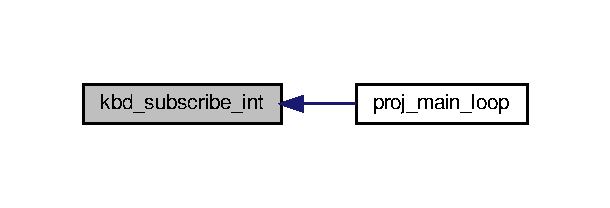
\includegraphics[width=293pt]{group__keyboard_ga4ac9231a99a664d6a9f0b69767e0d707_icgraph}
\end{center}
\end{figure}
\mbox{\Hypertarget{group__keyboard_gaee0a7b54ee426fade9c780418d110fe0}\label{group__keyboard_gaee0a7b54ee426fade9c780418d110fe0}} 
\index{Keyboard@{Keyboard}!kbd\+\_\+unsubscribe\+\_\+int@{kbd\+\_\+unsubscribe\+\_\+int}}
\index{kbd\+\_\+unsubscribe\+\_\+int@{kbd\+\_\+unsubscribe\+\_\+int}!Keyboard@{Keyboard}}
\subsubsection{\texorpdfstring{kbd\+\_\+unsubscribe\+\_\+int()}{kbd\_unsubscribe\_int()}}
{\footnotesize\ttfamily int() kbd\+\_\+unsubscribe\+\_\+int (\begin{DoxyParamCaption}{ }\end{DoxyParamCaption})}



Function that unsubscribes keyboard interruptions. 

\begin{DoxyReturn}{Returns}
Return 0 upon success 
\end{DoxyReturn}
Here is the caller graph for this function\+:\nopagebreak
\begin{figure}[H]
\begin{center}
\leavevmode
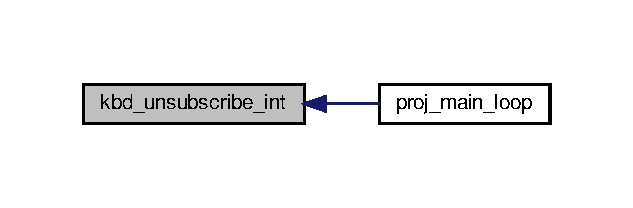
\includegraphics[width=304pt]{group__keyboard_gaee0a7b54ee426fade9c780418d110fe0_icgraph}
\end{center}
\end{figure}

\hypertarget{group__loading__xpms}{}\section{Loading\+\_\+xpms}
\label{group__loading__xpms}\index{Loading\+\_\+xpms@{Loading\+\_\+xpms}}
\subsection*{Functions}
\begin{DoxyCompactItemize}
\item 
int \hyperlink{group__loading__xpms_ga462cc2177dd9b043e5bd5689bbeaf868}{loading\+\_\+xpms} ()
\begin{DoxyCompactList}\small\item\em Loads all the xpms. \end{DoxyCompactList}\item 
xpm\+\_\+image\+\_\+t \hyperlink{group__loading__xpms_gada234fac1a8886b19a988eb80e99ef15}{decide\+\_\+rudolph} (uint16\+\_\+t pos\+\_\+x, uint16\+\_\+t pos\+\_\+y)
\begin{DoxyCompactList}\small\item\em Decides in what position the rudolph should be in (used to change rudolph\textquotesingle{}s eyes) \end{DoxyCompactList}\item 
xpm\+\_\+image\+\_\+t \hyperlink{group__loading__xpms_gafe3e8d1842749e3b8831f03eaff01c99}{decide\+\_\+sleep\+\_\+bar} (enum \hyperlink{group__types_ga210774229705ea136db591a108c52d39}{sleep\+\_\+bar} sb)
\begin{DoxyCompactList}\small\item\em Decides in what position the sleep bar should be in. \end{DoxyCompactList}\item 
xpm\+\_\+image\+\_\+t \hyperlink{group__loading__xpms_gad678e45b98e3cc05dca5b24dad2be564}{decide\+\_\+play\+\_\+bar} (enum \hyperlink{group__types_gaac3396b3def300539a13396b352b7fca}{play\+\_\+bar} pb)
\begin{DoxyCompactList}\small\item\em Decides in what position the fun bar should be in. \end{DoxyCompactList}\item 
xpm\+\_\+image\+\_\+t \hyperlink{group__loading__xpms_ga2cdb6cdede927ad5a784d34d47577acf}{decide\+\_\+food\+\_\+bar} (enum \hyperlink{group__types_ga68b33015e0d4635ee8ddb795eca9d963}{food\+\_\+bar} fb)
\begin{DoxyCompactList}\small\item\em Decides in what position the eat bar should be in. \end{DoxyCompactList}\item 
xpm\+\_\+image\+\_\+t \hyperlink{group__loading__xpms_ga5dbbff5de875a1305fdf7ed265fc73c8}{decide\+\_\+time} (enum \hyperlink{group__types_gad48fe05a3e5df355707b5a3fd6cf9d8e}{counter\+\_\+bar} c)
\begin{DoxyCompactList}\small\item\em Decides which xpm\+\_\+image\+\_\+t corresponds to the value of the counter of the minigame. \end{DoxyCompactList}\item 
enum \hyperlink{group__types_gabd8d88ed6ba2aef17eb45496d20be732}{score\+\_\+bar\+\_\+2} \hyperlink{group__loading__xpms_gac00aab23f7677ce5eee5748c335c994f}{event\+\_\+2} ()
\begin{DoxyCompactList}\small\item\em Decides which enum score\+\_\+bar\+\_\+2 corresponds to the value of dozens number of the scores. \end{DoxyCompactList}\item 
enum \hyperlink{group__types_gab5d0fdad1621cc17d1147dedd2e7a773}{score\+\_\+bar\+\_\+1} \hyperlink{group__loading__xpms_ga70f5397af0d313815b96cf662cd48f65}{event\+\_\+1} ()
\begin{DoxyCompactList}\small\item\em Decides which enum score\+\_\+bar\+\_\+1 corresponds to the value of units number of the scores. \end{DoxyCompactList}\item 
xpm\+\_\+image\+\_\+t \hyperlink{group__loading__xpms_ga2427af4195752a8d1c1f52ec6ade7735}{decide\+\_\+score\+\_\+2\+\_\+game} ()
\begin{DoxyCompactList}\small\item\em Decides which xpm\+\_\+image\+\_\+t corresponds to the dozens of the score of the minigame while playing. \end{DoxyCompactList}\item 
xpm\+\_\+image\+\_\+t \hyperlink{group__loading__xpms_ga3ff28b6df0ced24968db40bec439452e}{decide\+\_\+score\+\_\+2} ()
\begin{DoxyCompactList}\small\item\em Decides which xpm\+\_\+image\+\_\+t corresponds to the dozens of the score of the minigame after losing. \end{DoxyCompactList}\item 
xpm\+\_\+image\+\_\+t \hyperlink{group__loading__xpms_ga5808a0af7a81c9213427d1173ea4bfdb}{decide\+\_\+score\+\_\+1\+\_\+game} ()
\begin{DoxyCompactList}\small\item\em Decides which xpm\+\_\+image\+\_\+t corresponds to the units of the score of the minigame while playing. \end{DoxyCompactList}\item 
xpm\+\_\+image\+\_\+t \hyperlink{group__loading__xpms_ga49c14da168cc130190ad4808e0c889bf}{decide\+\_\+score\+\_\+1} ()
\begin{DoxyCompactList}\small\item\em Decides which xpm\+\_\+image\+\_\+t corresponds to the units of the score of the minigame after losing. \end{DoxyCompactList}\item 
xpm\+\_\+image\+\_\+t \hyperlink{group__loading__xpms_ga62a40150916b92b39ae83d800e3612f1}{decide\+\_\+hours} (\hyperlink{structrtc__time}{rtc\+\_\+time} $\ast$time)
\begin{DoxyCompactList}\small\item\em Decides which xpm\+\_\+image\+\_\+t corresponds to the R\+TC. \end{DoxyCompactList}\item 
xpm\+\_\+image\+\_\+t \hyperlink{group__loading__xpms_gae641aba4324c1f6c45eccb9d01822bd4}{decide\+\_\+minutes} (\hyperlink{structrtc__time}{rtc\+\_\+time} $\ast$time)
\begin{DoxyCompactList}\small\item\em Decides which xpm\+\_\+image\+\_\+t corresponds to the R\+TC. \end{DoxyCompactList}\end{DoxyCompactItemize}


\subsection{Detailed Description}
Functions used to help working with the xpms 

\subsection{Function Documentation}
\mbox{\Hypertarget{group__loading__xpms_ga2cdb6cdede927ad5a784d34d47577acf}\label{group__loading__xpms_ga2cdb6cdede927ad5a784d34d47577acf}} 
\index{Loading\+\_\+xpms@{Loading\+\_\+xpms}!decide\+\_\+food\+\_\+bar@{decide\+\_\+food\+\_\+bar}}
\index{decide\+\_\+food\+\_\+bar@{decide\+\_\+food\+\_\+bar}!Loading\+\_\+xpms@{Loading\+\_\+xpms}}
\subsubsection{\texorpdfstring{decide\+\_\+food\+\_\+bar()}{decide\_food\_bar()}}
{\footnotesize\ttfamily xpm\+\_\+image\+\_\+t decide\+\_\+food\+\_\+bar (\begin{DoxyParamCaption}\item[{enum \hyperlink{group__types_ga68b33015e0d4635ee8ddb795eca9d963}{food\+\_\+bar}}]{fb }\end{DoxyParamCaption})}



Decides in what position the eat bar should be in. 

The eat bar changes with time Depends on time and if the character is eating


\begin{DoxyParams}{Parameters}
{\em sb} & state of the current eat bar\\
\hline
\end{DoxyParams}
\begin{DoxyReturn}{Returns}
the xpm\+\_\+image\+\_\+t of the correspondent eat bar 
\end{DoxyReturn}
Here is the caller graph for this function\+:
\nopagebreak
\begin{figure}[H]
\begin{center}
\leavevmode
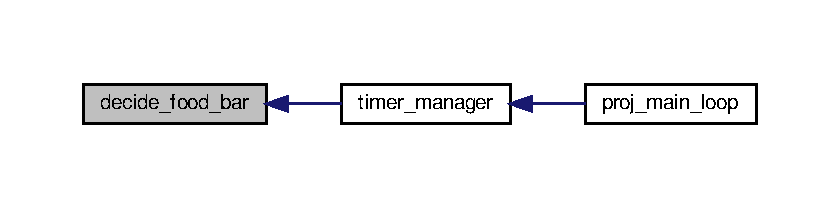
\includegraphics[width=350pt]{group__loading__xpms_ga2cdb6cdede927ad5a784d34d47577acf_icgraph}
\end{center}
\end{figure}
\mbox{\Hypertarget{group__loading__xpms_ga62a40150916b92b39ae83d800e3612f1}\label{group__loading__xpms_ga62a40150916b92b39ae83d800e3612f1}} 
\index{Loading\+\_\+xpms@{Loading\+\_\+xpms}!decide\+\_\+hours@{decide\+\_\+hours}}
\index{decide\+\_\+hours@{decide\+\_\+hours}!Loading\+\_\+xpms@{Loading\+\_\+xpms}}
\subsubsection{\texorpdfstring{decide\+\_\+hours()}{decide\_hours()}}
{\footnotesize\ttfamily xpm\+\_\+image\+\_\+t decide\+\_\+hours (\begin{DoxyParamCaption}\item[{\hyperlink{structrtc__time}{rtc\+\_\+time} $\ast$}]{time }\end{DoxyParamCaption})}



Decides which xpm\+\_\+image\+\_\+t corresponds to the R\+TC. 

Depends on the time of the computer


\begin{DoxyParams}{Parameters}
{\em time} & pointer to struct that has the value of the hours, minutes and seconds detected by the R\+TC\\
\hline
\end{DoxyParams}
\begin{DoxyReturn}{Returns}
the xpm\+\_\+image\+\_\+t of the correspondent hours (equal to the hours of the R\+TC) 
\end{DoxyReturn}
Here is the caller graph for this function\+:
\nopagebreak
\begin{figure}[H]
\begin{center}
\leavevmode
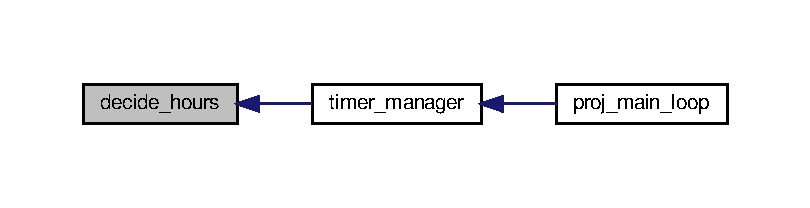
\includegraphics[width=350pt]{group__loading__xpms_ga62a40150916b92b39ae83d800e3612f1_icgraph}
\end{center}
\end{figure}
\mbox{\Hypertarget{group__loading__xpms_gae641aba4324c1f6c45eccb9d01822bd4}\label{group__loading__xpms_gae641aba4324c1f6c45eccb9d01822bd4}} 
\index{Loading\+\_\+xpms@{Loading\+\_\+xpms}!decide\+\_\+minutes@{decide\+\_\+minutes}}
\index{decide\+\_\+minutes@{decide\+\_\+minutes}!Loading\+\_\+xpms@{Loading\+\_\+xpms}}
\subsubsection{\texorpdfstring{decide\+\_\+minutes()}{decide\_minutes()}}
{\footnotesize\ttfamily xpm\+\_\+image\+\_\+t decide\+\_\+minutes (\begin{DoxyParamCaption}\item[{\hyperlink{structrtc__time}{rtc\+\_\+time} $\ast$}]{time }\end{DoxyParamCaption})}



Decides which xpm\+\_\+image\+\_\+t corresponds to the R\+TC. 

Depends on the time of the computer


\begin{DoxyParams}{Parameters}
{\em time} & pointer to struct that has the value of the hours, minutes and seconds detected by the R\+TC\\
\hline
\end{DoxyParams}
\begin{DoxyReturn}{Returns}
the xpm\+\_\+image\+\_\+t of the correspondent minutes (equal to the minutes of the R\+TC) 
\end{DoxyReturn}
Here is the caller graph for this function\+:
\nopagebreak
\begin{figure}[H]
\begin{center}
\leavevmode
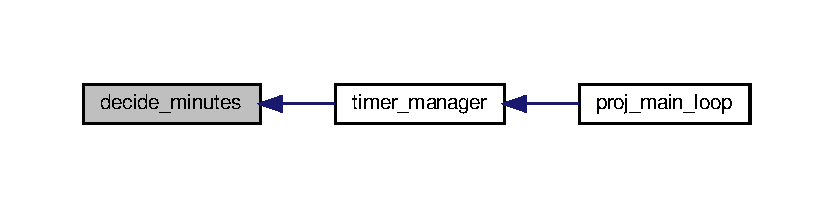
\includegraphics[width=350pt]{group__loading__xpms_gae641aba4324c1f6c45eccb9d01822bd4_icgraph}
\end{center}
\end{figure}
\mbox{\Hypertarget{group__loading__xpms_gad678e45b98e3cc05dca5b24dad2be564}\label{group__loading__xpms_gad678e45b98e3cc05dca5b24dad2be564}} 
\index{Loading\+\_\+xpms@{Loading\+\_\+xpms}!decide\+\_\+play\+\_\+bar@{decide\+\_\+play\+\_\+bar}}
\index{decide\+\_\+play\+\_\+bar@{decide\+\_\+play\+\_\+bar}!Loading\+\_\+xpms@{Loading\+\_\+xpms}}
\subsubsection{\texorpdfstring{decide\+\_\+play\+\_\+bar()}{decide\_play\_bar()}}
{\footnotesize\ttfamily xpm\+\_\+image\+\_\+t decide\+\_\+play\+\_\+bar (\begin{DoxyParamCaption}\item[{enum \hyperlink{group__types_gaac3396b3def300539a13396b352b7fca}{play\+\_\+bar}}]{pb }\end{DoxyParamCaption})}



Decides in what position the fun bar should be in. 

The fun bar changes with time Depends on time and if the character is playing


\begin{DoxyParams}{Parameters}
{\em sb} & state of the current play bar\\
\hline
\end{DoxyParams}
\begin{DoxyReturn}{Returns}
the xpm\+\_\+image\+\_\+t of the correspondent play bar 
\end{DoxyReturn}
Here is the caller graph for this function\+:
\nopagebreak
\begin{figure}[H]
\begin{center}
\leavevmode
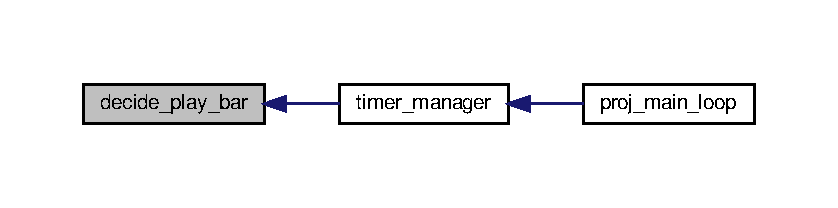
\includegraphics[width=350pt]{group__loading__xpms_gad678e45b98e3cc05dca5b24dad2be564_icgraph}
\end{center}
\end{figure}
\mbox{\Hypertarget{group__loading__xpms_gada234fac1a8886b19a988eb80e99ef15}\label{group__loading__xpms_gada234fac1a8886b19a988eb80e99ef15}} 
\index{Loading\+\_\+xpms@{Loading\+\_\+xpms}!decide\+\_\+rudolph@{decide\+\_\+rudolph}}
\index{decide\+\_\+rudolph@{decide\+\_\+rudolph}!Loading\+\_\+xpms@{Loading\+\_\+xpms}}
\subsubsection{\texorpdfstring{decide\+\_\+rudolph()}{decide\_rudolph()}}
{\footnotesize\ttfamily xpm\+\_\+image\+\_\+t decide\+\_\+rudolph (\begin{DoxyParamCaption}\item[{uint16\+\_\+t}]{pos\+\_\+x,  }\item[{uint16\+\_\+t}]{pos\+\_\+y }\end{DoxyParamCaption})}



Decides in what position the rudolph should be in (used to change rudolph\textquotesingle{}s eyes) 

Depends on the mouse postion


\begin{DoxyParams}{Parameters}
{\em pos\+\_\+x} & position x of the mouse \\
\hline
{\em pos\+\_\+y} & position y of the mouse\\
\hline
\end{DoxyParams}
\begin{DoxyReturn}{Returns}
the xpm\+\_\+image\+\_\+t of the correspondent rudolph position 
\end{DoxyReturn}
Here is the caller graph for this function\+:
\nopagebreak
\begin{figure}[H]
\begin{center}
\leavevmode
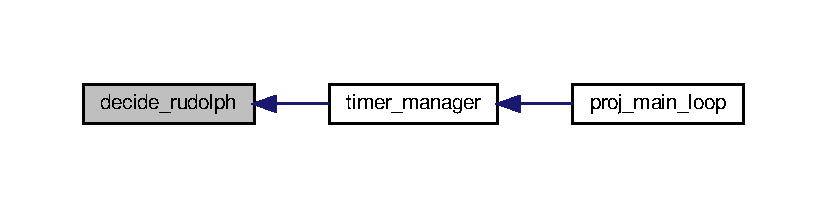
\includegraphics[width=350pt]{group__loading__xpms_gada234fac1a8886b19a988eb80e99ef15_icgraph}
\end{center}
\end{figure}
\mbox{\Hypertarget{group__loading__xpms_ga49c14da168cc130190ad4808e0c889bf}\label{group__loading__xpms_ga49c14da168cc130190ad4808e0c889bf}} 
\index{Loading\+\_\+xpms@{Loading\+\_\+xpms}!decide\+\_\+score\+\_\+1@{decide\+\_\+score\+\_\+1}}
\index{decide\+\_\+score\+\_\+1@{decide\+\_\+score\+\_\+1}!Loading\+\_\+xpms@{Loading\+\_\+xpms}}
\subsubsection{\texorpdfstring{decide\+\_\+score\+\_\+1()}{decide\_score\_1()}}
{\footnotesize\ttfamily xpm\+\_\+image\+\_\+t decide\+\_\+score\+\_\+1 (\begin{DoxyParamCaption}{ }\end{DoxyParamCaption})}



Decides which xpm\+\_\+image\+\_\+t corresponds to the units of the score of the minigame after losing. 

The counter changes with the value of the enum returned in \hyperlink{group__loading__xpms_ga70f5397af0d313815b96cf662cd48f65}{event\+\_\+1()} Depends on time

\begin{DoxyReturn}{Returns}
the xpm\+\_\+image\+\_\+t of the correspondent value of the units out of the minigame 
\end{DoxyReturn}
Here is the call graph for this function\+:
\nopagebreak
\begin{figure}[H]
\begin{center}
\leavevmode
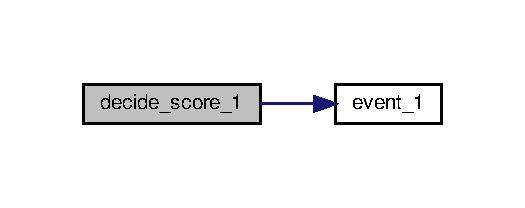
\includegraphics[width=252pt]{group__loading__xpms_ga49c14da168cc130190ad4808e0c889bf_cgraph}
\end{center}
\end{figure}
Here is the caller graph for this function\+:
\nopagebreak
\begin{figure}[H]
\begin{center}
\leavevmode
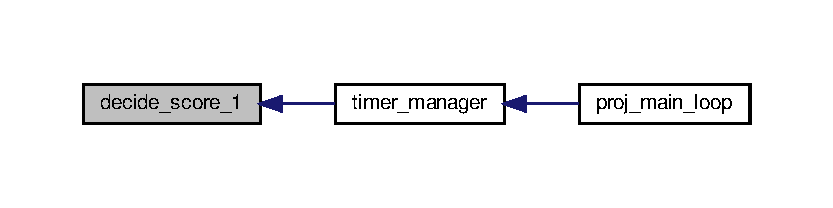
\includegraphics[width=350pt]{group__loading__xpms_ga49c14da168cc130190ad4808e0c889bf_icgraph}
\end{center}
\end{figure}
\mbox{\Hypertarget{group__loading__xpms_ga5808a0af7a81c9213427d1173ea4bfdb}\label{group__loading__xpms_ga5808a0af7a81c9213427d1173ea4bfdb}} 
\index{Loading\+\_\+xpms@{Loading\+\_\+xpms}!decide\+\_\+score\+\_\+1\+\_\+game@{decide\+\_\+score\+\_\+1\+\_\+game}}
\index{decide\+\_\+score\+\_\+1\+\_\+game@{decide\+\_\+score\+\_\+1\+\_\+game}!Loading\+\_\+xpms@{Loading\+\_\+xpms}}
\subsubsection{\texorpdfstring{decide\+\_\+score\+\_\+1\+\_\+game()}{decide\_score\_1\_game()}}
{\footnotesize\ttfamily xpm\+\_\+image\+\_\+t decide\+\_\+score\+\_\+1\+\_\+game (\begin{DoxyParamCaption}{ }\end{DoxyParamCaption})}



Decides which xpm\+\_\+image\+\_\+t corresponds to the units of the score of the minigame while playing. 

The counter changes with the value of the enum returned in \hyperlink{group__loading__xpms_ga70f5397af0d313815b96cf662cd48f65}{event\+\_\+1()} Depends on time

\begin{DoxyReturn}{Returns}
the xpm\+\_\+image\+\_\+t of the correspondent value of the units in the minigame 
\end{DoxyReturn}
Here is the call graph for this function\+:
\nopagebreak
\begin{figure}[H]
\begin{center}
\leavevmode
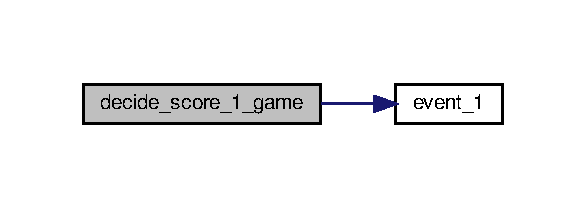
\includegraphics[width=281pt]{group__loading__xpms_ga5808a0af7a81c9213427d1173ea4bfdb_cgraph}
\end{center}
\end{figure}
Here is the caller graph for this function\+:
\nopagebreak
\begin{figure}[H]
\begin{center}
\leavevmode
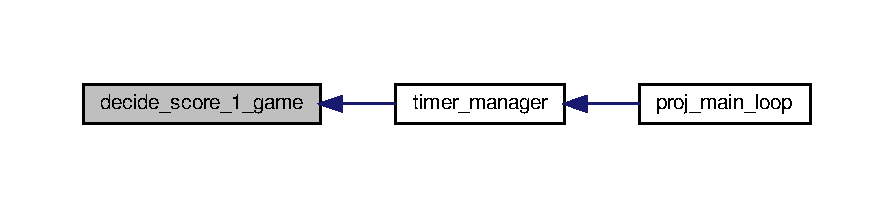
\includegraphics[width=350pt]{group__loading__xpms_ga5808a0af7a81c9213427d1173ea4bfdb_icgraph}
\end{center}
\end{figure}
\mbox{\Hypertarget{group__loading__xpms_ga3ff28b6df0ced24968db40bec439452e}\label{group__loading__xpms_ga3ff28b6df0ced24968db40bec439452e}} 
\index{Loading\+\_\+xpms@{Loading\+\_\+xpms}!decide\+\_\+score\+\_\+2@{decide\+\_\+score\+\_\+2}}
\index{decide\+\_\+score\+\_\+2@{decide\+\_\+score\+\_\+2}!Loading\+\_\+xpms@{Loading\+\_\+xpms}}
\subsubsection{\texorpdfstring{decide\+\_\+score\+\_\+2()}{decide\_score\_2()}}
{\footnotesize\ttfamily xpm\+\_\+image\+\_\+t decide\+\_\+score\+\_\+2 (\begin{DoxyParamCaption}{ }\end{DoxyParamCaption})}



Decides which xpm\+\_\+image\+\_\+t corresponds to the dozens of the score of the minigame after losing. 

The counter changes with the value of the enum returned in \hyperlink{group__loading__xpms_gac00aab23f7677ce5eee5748c335c994f}{event\+\_\+2()} Depends on time

\begin{DoxyReturn}{Returns}
the xpm\+\_\+image\+\_\+t of the correspondent value of the dozens out of the minigame 
\end{DoxyReturn}
Here is the call graph for this function\+:
\nopagebreak
\begin{figure}[H]
\begin{center}
\leavevmode
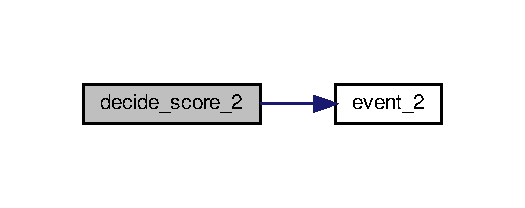
\includegraphics[width=252pt]{group__loading__xpms_ga3ff28b6df0ced24968db40bec439452e_cgraph}
\end{center}
\end{figure}
Here is the caller graph for this function\+:
\nopagebreak
\begin{figure}[H]
\begin{center}
\leavevmode
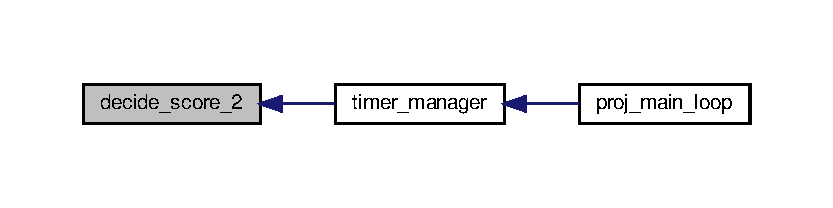
\includegraphics[width=350pt]{group__loading__xpms_ga3ff28b6df0ced24968db40bec439452e_icgraph}
\end{center}
\end{figure}
\mbox{\Hypertarget{group__loading__xpms_ga2427af4195752a8d1c1f52ec6ade7735}\label{group__loading__xpms_ga2427af4195752a8d1c1f52ec6ade7735}} 
\index{Loading\+\_\+xpms@{Loading\+\_\+xpms}!decide\+\_\+score\+\_\+2\+\_\+game@{decide\+\_\+score\+\_\+2\+\_\+game}}
\index{decide\+\_\+score\+\_\+2\+\_\+game@{decide\+\_\+score\+\_\+2\+\_\+game}!Loading\+\_\+xpms@{Loading\+\_\+xpms}}
\subsubsection{\texorpdfstring{decide\+\_\+score\+\_\+2\+\_\+game()}{decide\_score\_2\_game()}}
{\footnotesize\ttfamily xpm\+\_\+image\+\_\+t decide\+\_\+score\+\_\+2\+\_\+game (\begin{DoxyParamCaption}{ }\end{DoxyParamCaption})}



Decides which xpm\+\_\+image\+\_\+t corresponds to the dozens of the score of the minigame while playing. 

The counter changes with the value of the enum returned in \hyperlink{group__loading__xpms_gac00aab23f7677ce5eee5748c335c994f}{event\+\_\+2()} Depends on time

\begin{DoxyReturn}{Returns}
the xpm\+\_\+image\+\_\+t of the correspondent value of the dozens in the minigame 
\end{DoxyReturn}
Here is the call graph for this function\+:
\nopagebreak
\begin{figure}[H]
\begin{center}
\leavevmode
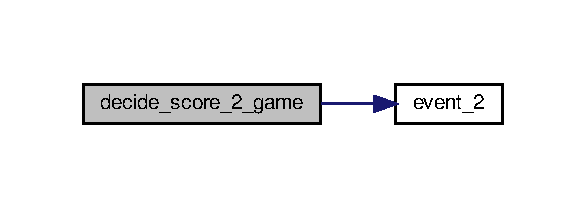
\includegraphics[width=281pt]{group__loading__xpms_ga2427af4195752a8d1c1f52ec6ade7735_cgraph}
\end{center}
\end{figure}
Here is the caller graph for this function\+:
\nopagebreak
\begin{figure}[H]
\begin{center}
\leavevmode
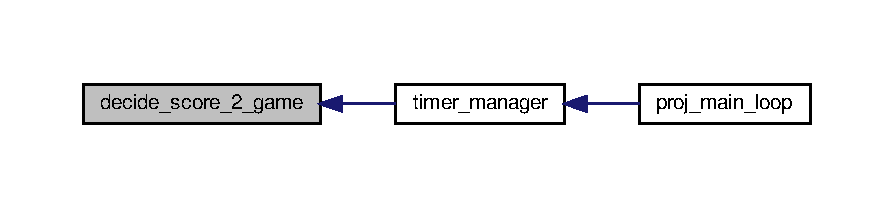
\includegraphics[width=350pt]{group__loading__xpms_ga2427af4195752a8d1c1f52ec6ade7735_icgraph}
\end{center}
\end{figure}
\mbox{\Hypertarget{group__loading__xpms_gafe3e8d1842749e3b8831f03eaff01c99}\label{group__loading__xpms_gafe3e8d1842749e3b8831f03eaff01c99}} 
\index{Loading\+\_\+xpms@{Loading\+\_\+xpms}!decide\+\_\+sleep\+\_\+bar@{decide\+\_\+sleep\+\_\+bar}}
\index{decide\+\_\+sleep\+\_\+bar@{decide\+\_\+sleep\+\_\+bar}!Loading\+\_\+xpms@{Loading\+\_\+xpms}}
\subsubsection{\texorpdfstring{decide\+\_\+sleep\+\_\+bar()}{decide\_sleep\_bar()}}
{\footnotesize\ttfamily xpm\+\_\+image\+\_\+t decide\+\_\+sleep\+\_\+bar (\begin{DoxyParamCaption}\item[{enum \hyperlink{group__types_ga210774229705ea136db591a108c52d39}{sleep\+\_\+bar}}]{sb }\end{DoxyParamCaption})}



Decides in what position the sleep bar should be in. 

The sleep bar changes with time Depends on time and if the character is sleeping or not


\begin{DoxyParams}{Parameters}
{\em sb} & state of the current sleep bar\\
\hline
\end{DoxyParams}
\begin{DoxyReturn}{Returns}
the xpm\+\_\+image\+\_\+t of the correspondent sleep bar 
\end{DoxyReturn}
Here is the caller graph for this function\+:
\nopagebreak
\begin{figure}[H]
\begin{center}
\leavevmode
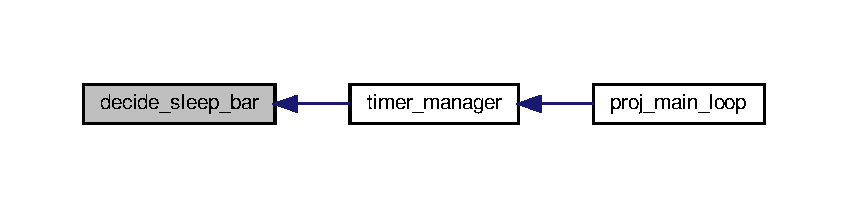
\includegraphics[width=350pt]{group__loading__xpms_gafe3e8d1842749e3b8831f03eaff01c99_icgraph}
\end{center}
\end{figure}
\mbox{\Hypertarget{group__loading__xpms_ga5dbbff5de875a1305fdf7ed265fc73c8}\label{group__loading__xpms_ga5dbbff5de875a1305fdf7ed265fc73c8}} 
\index{Loading\+\_\+xpms@{Loading\+\_\+xpms}!decide\+\_\+time@{decide\+\_\+time}}
\index{decide\+\_\+time@{decide\+\_\+time}!Loading\+\_\+xpms@{Loading\+\_\+xpms}}
\subsubsection{\texorpdfstring{decide\+\_\+time()}{decide\_time()}}
{\footnotesize\ttfamily xpm\+\_\+image\+\_\+t decide\+\_\+time (\begin{DoxyParamCaption}\item[{enum \hyperlink{group__types_gad48fe05a3e5df355707b5a3fd6cf9d8e}{counter\+\_\+bar}}]{c }\end{DoxyParamCaption})}



Decides which xpm\+\_\+image\+\_\+t corresponds to the value of the counter of the minigame. 

The counter changes with time Depends on time


\begin{DoxyParams}{Parameters}
{\em c} & current time\\
\hline
\end{DoxyParams}
\begin{DoxyReturn}{Returns}
the xpm\+\_\+image\+\_\+t of the correspondent counter value 
\end{DoxyReturn}
Here is the caller graph for this function\+:
\nopagebreak
\begin{figure}[H]
\begin{center}
\leavevmode
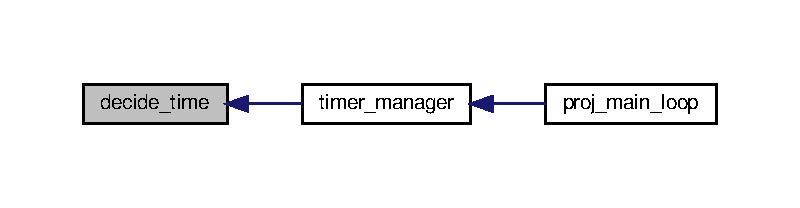
\includegraphics[width=350pt]{group__loading__xpms_ga5dbbff5de875a1305fdf7ed265fc73c8_icgraph}
\end{center}
\end{figure}
\mbox{\Hypertarget{group__loading__xpms_ga70f5397af0d313815b96cf662cd48f65}\label{group__loading__xpms_ga70f5397af0d313815b96cf662cd48f65}} 
\index{Loading\+\_\+xpms@{Loading\+\_\+xpms}!event\+\_\+1@{event\+\_\+1}}
\index{event\+\_\+1@{event\+\_\+1}!Loading\+\_\+xpms@{Loading\+\_\+xpms}}
\subsubsection{\texorpdfstring{event\+\_\+1()}{event\_1()}}
{\footnotesize\ttfamily enum \hyperlink{group__types_gab5d0fdad1621cc17d1147dedd2e7a773}{score\+\_\+bar\+\_\+1} event\+\_\+1 (\begin{DoxyParamCaption}{ }\end{DoxyParamCaption})}



Decides which enum score\+\_\+bar\+\_\+1 corresponds to the value of units number of the scores. 

This value changes when the character presses the correct key 1 time

\begin{DoxyReturn}{Returns}
enum value of the units number for the score 
\end{DoxyReturn}
Here is the caller graph for this function\+:
\nopagebreak
\begin{figure}[H]
\begin{center}
\leavevmode
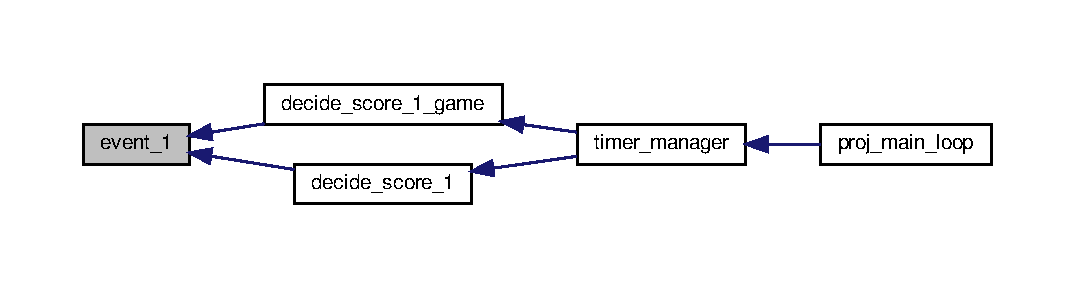
\includegraphics[width=350pt]{group__loading__xpms_ga70f5397af0d313815b96cf662cd48f65_icgraph}
\end{center}
\end{figure}
\mbox{\Hypertarget{group__loading__xpms_gac00aab23f7677ce5eee5748c335c994f}\label{group__loading__xpms_gac00aab23f7677ce5eee5748c335c994f}} 
\index{Loading\+\_\+xpms@{Loading\+\_\+xpms}!event\+\_\+2@{event\+\_\+2}}
\index{event\+\_\+2@{event\+\_\+2}!Loading\+\_\+xpms@{Loading\+\_\+xpms}}
\subsubsection{\texorpdfstring{event\+\_\+2()}{event\_2()}}
{\footnotesize\ttfamily enum \hyperlink{group__types_gabd8d88ed6ba2aef17eb45496d20be732}{score\+\_\+bar\+\_\+2} event\+\_\+2 (\begin{DoxyParamCaption}{ }\end{DoxyParamCaption})}



Decides which enum score\+\_\+bar\+\_\+2 corresponds to the value of dozens number of the scores. 

This value changes when the character presses the correct key 10 times

\begin{DoxyReturn}{Returns}
enum value of the dozens number for the score 
\end{DoxyReturn}
Here is the caller graph for this function\+:
\nopagebreak
\begin{figure}[H]
\begin{center}
\leavevmode
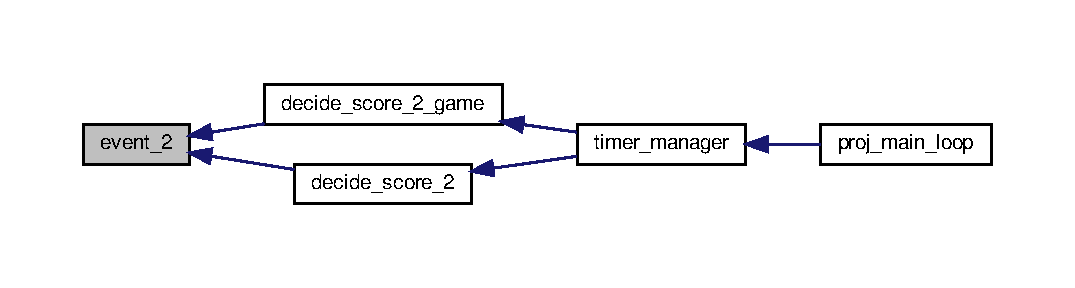
\includegraphics[width=350pt]{group__loading__xpms_gac00aab23f7677ce5eee5748c335c994f_icgraph}
\end{center}
\end{figure}
\mbox{\Hypertarget{group__loading__xpms_ga462cc2177dd9b043e5bd5689bbeaf868}\label{group__loading__xpms_ga462cc2177dd9b043e5bd5689bbeaf868}} 
\index{Loading\+\_\+xpms@{Loading\+\_\+xpms}!loading\+\_\+xpms@{loading\+\_\+xpms}}
\index{loading\+\_\+xpms@{loading\+\_\+xpms}!Loading\+\_\+xpms@{Loading\+\_\+xpms}}
\subsubsection{\texorpdfstring{loading\+\_\+xpms()}{loading\_xpms()}}
{\footnotesize\ttfamily int loading\+\_\+xpms (\begin{DoxyParamCaption}{ }\end{DoxyParamCaption})}



Loads all the xpms. 

\begin{DoxyReturn}{Returns}
Return 0 upon success 
\end{DoxyReturn}
Here is the caller graph for this function\+:\nopagebreak
\begin{figure}[H]
\begin{center}
\leavevmode
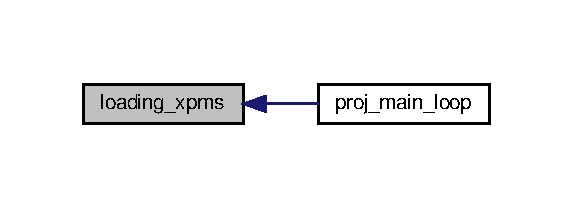
\includegraphics[width=275pt]{group__loading__xpms_ga462cc2177dd9b043e5bd5689bbeaf868_icgraph}
\end{center}
\end{figure}

\hypertarget{group__keyboard__macros}{}\section{Keyboard\+\_\+macros}
\label{group__keyboard__macros}\index{Keyboard\+\_\+macros@{Keyboard\+\_\+macros}}
\subsection*{Macros}
\begin{DoxyCompactItemize}
\item 
\mbox{\Hypertarget{group__keyboard__macros_ga45967c9e25447ba853cf6fb4ac545fe6}\label{group__keyboard__macros_ga45967c9e25447ba853cf6fb4ac545fe6}} 
\#define \hyperlink{group__keyboard__macros_ga45967c9e25447ba853cf6fb4ac545fe6}{O\+BF}~0x01
\begin{DoxyCompactList}\small\item\em status register bit 0 \end{DoxyCompactList}\item 
\mbox{\Hypertarget{group__keyboard__macros_ga307ab71673e26ec42b28a3bca05d4cb5}\label{group__keyboard__macros_ga307ab71673e26ec42b28a3bca05d4cb5}} 
\#define \hyperlink{group__keyboard__macros_ga307ab71673e26ec42b28a3bca05d4cb5}{P\+A\+R\+\_\+\+E\+RR}~0x80
\begin{DoxyCompactList}\small\item\em status register bit 7 \end{DoxyCompactList}\item 
\mbox{\Hypertarget{group__keyboard__macros_ga45ba202b05caf39795aeca91b0ae547e}\label{group__keyboard__macros_ga45ba202b05caf39795aeca91b0ae547e}} 
\#define \hyperlink{group__keyboard__macros_ga45ba202b05caf39795aeca91b0ae547e}{T\+I\+M\+E\+O\+UT}~0x40
\begin{DoxyCompactList}\small\item\em status register bit 6 \end{DoxyCompactList}\item 
\mbox{\Hypertarget{group__keyboard__macros_ga1b41fd2be63532d4ab910f8b256c3811}\label{group__keyboard__macros_ga1b41fd2be63532d4ab910f8b256c3811}} 
\#define \hyperlink{group__keyboard__macros_ga1b41fd2be63532d4ab910f8b256c3811}{A\+UX}~0x20
\begin{DoxyCompactList}\small\item\em status register bit 5 \end{DoxyCompactList}\item 
\mbox{\Hypertarget{group__keyboard__macros_ga03f542f1e0e2ba512c4ed189decfee3d}\label{group__keyboard__macros_ga03f542f1e0e2ba512c4ed189decfee3d}} 
\#define \hyperlink{group__keyboard__macros_ga03f542f1e0e2ba512c4ed189decfee3d}{I\+NH}~0x10
\begin{DoxyCompactList}\small\item\em status register bit 4 \end{DoxyCompactList}\item 
\mbox{\Hypertarget{group__keyboard__macros_ga2946bc30423c2a996eeafa49e995c30e}\label{group__keyboard__macros_ga2946bc30423c2a996eeafa49e995c30e}} 
\#define \hyperlink{group__keyboard__macros_ga2946bc30423c2a996eeafa49e995c30e}{A2}~0x08
\begin{DoxyCompactList}\small\item\em status register bit 3 \end{DoxyCompactList}\item 
\mbox{\Hypertarget{group__keyboard__macros_gae3d9f52a1a315303ad04f0576bd42a25}\label{group__keyboard__macros_gae3d9f52a1a315303ad04f0576bd42a25}} 
\#define \hyperlink{group__keyboard__macros_gae3d9f52a1a315303ad04f0576bd42a25}{S\+YS}~0x04
\begin{DoxyCompactList}\small\item\em status register bit 2 \end{DoxyCompactList}\item 
\mbox{\Hypertarget{group__keyboard__macros_ga3c48b10907056351582baf9f6478598e}\label{group__keyboard__macros_ga3c48b10907056351582baf9f6478598e}} 
\#define \hyperlink{group__keyboard__macros_ga3c48b10907056351582baf9f6478598e}{I\+BF}~0x02
\begin{DoxyCompactList}\small\item\em status register bit 1 \end{DoxyCompactList}\item 
\mbox{\Hypertarget{group__keyboard__macros_ga5c1072213ce8d8cd43628c4319ae0391}\label{group__keyboard__macros_ga5c1072213ce8d8cd43628c4319ae0391}} 
\#define {\bfseries K\+B\+D\+\_\+\+I\+RQ}~1
\item 
\mbox{\Hypertarget{group__keyboard__macros_gacfb42dde389e8ca36ab267002fbf5c6a}\label{group__keyboard__macros_gacfb42dde389e8ca36ab267002fbf5c6a}} 
\#define \hyperlink{group__keyboard__macros_gacfb42dde389e8ca36ab267002fbf5c6a}{O\+U\+T\+\_\+\+B\+UF}~0x60
\begin{DoxyCompactList}\small\item\em output buffer \end{DoxyCompactList}\item 
\mbox{\Hypertarget{group__keyboard__macros_ga783be5698cf07b1daaf126ef89c19063}\label{group__keyboard__macros_ga783be5698cf07b1daaf126ef89c19063}} 
\#define \hyperlink{group__keyboard__macros_ga783be5698cf07b1daaf126ef89c19063}{I\+N\+\_\+\+B\+UF}~0x60
\begin{DoxyCompactList}\small\item\em input buffer \end{DoxyCompactList}\item 
\mbox{\Hypertarget{group__keyboard__macros_ga89c4d098b53809674457b1660b1af780}\label{group__keyboard__macros_ga89c4d098b53809674457b1660b1af780}} 
\#define \hyperlink{group__keyboard__macros_ga89c4d098b53809674457b1660b1af780}{S\+T\+A\+T\+\_\+\+R\+EG}~0x64
\begin{DoxyCompactList}\small\item\em Status register. \end{DoxyCompactList}\item 
\mbox{\Hypertarget{group__keyboard__macros_ga6d57c7927a10f638c83046b52c8caac9}\label{group__keyboard__macros_ga6d57c7927a10f638c83046b52c8caac9}} 
\#define \hyperlink{group__keyboard__macros_ga6d57c7927a10f638c83046b52c8caac9}{K\+B\+C\+\_\+\+C\+M\+D\+\_\+\+R\+EG}~0x64
\begin{DoxyCompactList}\small\item\em kbc command register \end{DoxyCompactList}\item 
\mbox{\Hypertarget{group__keyboard__macros_ga21623e2a5501c821da54dd76ffc1d077}\label{group__keyboard__macros_ga21623e2a5501c821da54dd76ffc1d077}} 
\#define \hyperlink{group__keyboard__macros_ga21623e2a5501c821da54dd76ffc1d077}{R\+E\+A\+D\+\_\+\+C\+MD}~0x20
\begin{DoxyCompactList}\small\item\em read command byte \end{DoxyCompactList}\item 
\mbox{\Hypertarget{group__keyboard__macros_gaf792feb13ae0c1eab8f95f64c8baa96d}\label{group__keyboard__macros_gaf792feb13ae0c1eab8f95f64c8baa96d}} 
\#define \hyperlink{group__keyboard__macros_gaf792feb13ae0c1eab8f95f64c8baa96d}{W\+R\+I\+T\+E\+\_\+\+C\+MD}~0x60
\begin{DoxyCompactList}\small\item\em write command byte \end{DoxyCompactList}\item 
\mbox{\Hypertarget{group__keyboard__macros_ga54db80d887c9139084b1a66243fa3f72}\label{group__keyboard__macros_ga54db80d887c9139084b1a66243fa3f72}} 
\#define \hyperlink{group__keyboard__macros_ga54db80d887c9139084b1a66243fa3f72}{E\+N\+T\+E\+R\+\_\+\+B\+R\+E\+A\+K\+\_\+\+C\+O\+DE}~0x9c
\begin{DoxyCompactList}\small\item\em enter break code \end{DoxyCompactList}\item 
\mbox{\Hypertarget{group__keyboard__macros_ga71a8fdf08c766bfa05e6524f64d16ed0}\label{group__keyboard__macros_ga71a8fdf08c766bfa05e6524f64d16ed0}} 
\#define \hyperlink{group__keyboard__macros_ga71a8fdf08c766bfa05e6524f64d16ed0}{E\+R\+A\+S\+E\+\_\+\+B\+R\+E\+A\+K\+\_\+\+C\+O\+DE}~0x8e
\begin{DoxyCompactList}\small\item\em erase break code \end{DoxyCompactList}\item 
\mbox{\Hypertarget{group__keyboard__macros_ga592dfdf397b21913348b4dd6b7759b2d}\label{group__keyboard__macros_ga592dfdf397b21913348b4dd6b7759b2d}} 
\#define \hyperlink{group__keyboard__macros_ga592dfdf397b21913348b4dd6b7759b2d}{E\+S\+C\+\_\+\+B\+R\+E\+A\+K\+\_\+\+C\+O\+DE}~0x81
\begin{DoxyCompactList}\small\item\em Break code of the Esc key. \end{DoxyCompactList}\item 
\mbox{\Hypertarget{group__keyboard__macros_ga2877405e9b042d1e29cc09bcc8daccfa}\label{group__keyboard__macros_ga2877405e9b042d1e29cc09bcc8daccfa}} 
\#define \hyperlink{group__keyboard__macros_ga2877405e9b042d1e29cc09bcc8daccfa}{T\+W\+O\+\_\+\+B\+Y\+T\+E\+\_\+\+C\+O\+DE}~0xe0
\begin{DoxyCompactList}\small\item\em To test when a code is two bytes long. \end{DoxyCompactList}\item 
\mbox{\Hypertarget{group__keyboard__macros_ga1a522aa19bcb695a9df30032a893bee3}\label{group__keyboard__macros_ga1a522aa19bcb695a9df30032a893bee3}} 
\#define \hyperlink{group__keyboard__macros_ga1a522aa19bcb695a9df30032a893bee3}{D\+E\+L\+A\+Y\+\_\+\+US}~20000
\begin{DoxyCompactList}\small\item\em delay used in the delay function \end{DoxyCompactList}\item 
\mbox{\Hypertarget{group__keyboard__macros_ga9b5c2e5a8f5495e736c3ff9cf6945ce6}\label{group__keyboard__macros_ga9b5c2e5a8f5495e736c3ff9cf6945ce6}} 
\#define \hyperlink{group__keyboard__macros_ga9b5c2e5a8f5495e736c3ff9cf6945ce6}{R\+I\+G\+H\+T\+\_\+\+A\+R\+R\+O\+W\+\_\+\+B\+R\+E\+A\+K\+\_\+\+C\+O\+DE}~0x\+C\+D\+E0
\begin{DoxyCompactList}\small\item\em right arrow break code \end{DoxyCompactList}\item 
\mbox{\Hypertarget{group__keyboard__macros_gad7e318af05b90ab67821d521b916fe72}\label{group__keyboard__macros_gad7e318af05b90ab67821d521b916fe72}} 
\#define \hyperlink{group__keyboard__macros_gad7e318af05b90ab67821d521b916fe72}{L\+E\+F\+T\+\_\+\+A\+R\+R\+O\+W\+\_\+\+B\+R\+E\+A\+K\+\_\+\+C\+O\+DE}~0x\+C\+B\+E0
\begin{DoxyCompactList}\small\item\em left arrow break code \end{DoxyCompactList}\item 
\mbox{\Hypertarget{group__keyboard__macros_ga6b3bc710b60263bd76130540a24b74b6}\label{group__keyboard__macros_ga6b3bc710b60263bd76130540a24b74b6}} 
\#define \hyperlink{group__keyboard__macros_ga6b3bc710b60263bd76130540a24b74b6}{A\+\_\+\+B\+R\+E\+A\+K\+\_\+\+C\+O\+DE}~0x9E
\begin{DoxyCompactList}\small\item\em a break code \end{DoxyCompactList}\item 
\mbox{\Hypertarget{group__keyboard__macros_gaeb7fb0b62eabc29ca24eb9ce77b07152}\label{group__keyboard__macros_gaeb7fb0b62eabc29ca24eb9ce77b07152}} 
\#define \hyperlink{group__keyboard__macros_gaeb7fb0b62eabc29ca24eb9ce77b07152}{D\+\_\+\+B\+R\+E\+A\+K\+\_\+\+C\+O\+DE}~0x\+A0
\begin{DoxyCompactList}\small\item\em d break code \end{DoxyCompactList}\end{DoxyCompactItemize}


\subsection{Detailed Description}
Keyboard macros 
\hypertarget{group___project}{}\section{Macros}
\label{group___project}\index{Macros@{Macros}}
Collaboration diagram for Macros\+:\nopagebreak
\begin{figure}[H]
\begin{center}
\leavevmode
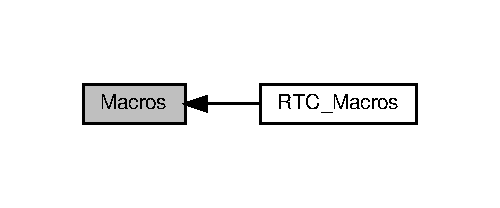
\includegraphics[width=240pt]{group___project}
\end{center}
\end{figure}
\subsection*{Modules}
\begin{DoxyCompactItemize}
\item 
\hyperlink{group___r_t_c___macros}{R\+T\+C\+\_\+\+Macros}
\end{DoxyCompactItemize}
\subsection*{Macros}
\begin{DoxyCompactItemize}
\item 
\mbox{\Hypertarget{group___project_ga2bd150533f839ae2c693ab76e55799c1}\label{group___project_ga2bd150533f839ae2c693ab76e55799c1}} 
\#define \hyperlink{group___project_ga2bd150533f839ae2c693ab76e55799c1}{C\+H\+A\+R\+\_\+X}~324
\begin{DoxyCompactList}\small\item\em character position (x) \end{DoxyCompactList}\item 
\mbox{\Hypertarget{group___project_ga9528c0d136b8c20810d6aac309767e28}\label{group___project_ga9528c0d136b8c20810d6aac309767e28}} 
\#define \hyperlink{group___project_ga9528c0d136b8c20810d6aac309767e28}{C\+H\+A\+R\+\_\+Y}~313
\begin{DoxyCompactList}\small\item\em character position (y) \end{DoxyCompactList}\item 
\mbox{\Hypertarget{group___project_ga93acb4f08ef430ffe2ff6d18f37adfde}\label{group___project_ga93acb4f08ef430ffe2ff6d18f37adfde}} 
\#define \hyperlink{group___project_ga93acb4f08ef430ffe2ff6d18f37adfde}{M\+I\+N\+\_\+\+E\+S\+Q\+U\+E\+R\+D\+A\+\_\+X}~0
\begin{DoxyCompactList}\small\item\em minimum value of the left rectangle of the screen (x) \end{DoxyCompactList}\item 
\mbox{\Hypertarget{group___project_ga4463271563a547fe21abbfa253d7ca6b}\label{group___project_ga4463271563a547fe21abbfa253d7ca6b}} 
\#define \hyperlink{group___project_ga4463271563a547fe21abbfa253d7ca6b}{M\+A\+X\+\_\+\+E\+S\+Q\+U\+E\+R\+D\+A\+\_\+X}~341
\begin{DoxyCompactList}\small\item\em minimum value of the left rectangle of the screen (x) \end{DoxyCompactList}\item 
\mbox{\Hypertarget{group___project_ga2de13b7e3c25e2f8ad5720113ccf1c09}\label{group___project_ga2de13b7e3c25e2f8ad5720113ccf1c09}} 
\#define \hyperlink{group___project_ga2de13b7e3c25e2f8ad5720113ccf1c09}{M\+I\+N\+\_\+\+M\+E\+I\+O\+\_\+X}~341
\begin{DoxyCompactList}\small\item\em minimum value of the center rectangle of the screen (x) \end{DoxyCompactList}\item 
\mbox{\Hypertarget{group___project_gaf2951cc1a396309759ae497a7f8db1e4}\label{group___project_gaf2951cc1a396309759ae497a7f8db1e4}} 
\#define \hyperlink{group___project_gaf2951cc1a396309759ae497a7f8db1e4}{M\+A\+X\+\_\+\+M\+E\+I\+O\+\_\+X}~682
\begin{DoxyCompactList}\small\item\em maximum value of the center rectangle of the screen (x) \end{DoxyCompactList}\item 
\mbox{\Hypertarget{group___project_ga2229ca24bc122bd9408689734320d096}\label{group___project_ga2229ca24bc122bd9408689734320d096}} 
\#define \hyperlink{group___project_ga2229ca24bc122bd9408689734320d096}{M\+I\+N\+\_\+\+D\+I\+R\+E\+I\+T\+A\+\_\+X}~682
\begin{DoxyCompactList}\small\item\em minimum value of the right rectangle of the screen (x) \end{DoxyCompactList}\item 
\mbox{\Hypertarget{group___project_ga0ea90e9c0e7cf279489dcb13ab3d8212}\label{group___project_ga0ea90e9c0e7cf279489dcb13ab3d8212}} 
\#define \hyperlink{group___project_ga0ea90e9c0e7cf279489dcb13ab3d8212}{M\+A\+X\+\_\+\+D\+I\+R\+E\+I\+T\+A\+\_\+X}~1024
\begin{DoxyCompactList}\small\item\em maximum value of the right rectangle of the screen (x) \end{DoxyCompactList}\item 
\mbox{\Hypertarget{group___project_gaf8aa68539c964feec74431936d6eaaa9}\label{group___project_gaf8aa68539c964feec74431936d6eaaa9}} 
\#define \hyperlink{group___project_gaf8aa68539c964feec74431936d6eaaa9}{M\+I\+N\+\_\+\+C\+I\+M\+A\+\_\+Y}~0
\begin{DoxyCompactList}\small\item\em minimum value of the top rectangle of the screen (y) \end{DoxyCompactList}\item 
\mbox{\Hypertarget{group___project_ga2e63ec1e993006b487719d1e8d6f87e2}\label{group___project_ga2e63ec1e993006b487719d1e8d6f87e2}} 
\#define \hyperlink{group___project_ga2e63ec1e993006b487719d1e8d6f87e2}{M\+A\+X\+\_\+\+C\+I\+M\+A\+\_\+Y}~384
\begin{DoxyCompactList}\small\item\em maximum value of the top rectangle of the screen (y) \end{DoxyCompactList}\item 
\mbox{\Hypertarget{group___project_gab180f7345963fc24a62a0b7308722a61}\label{group___project_gab180f7345963fc24a62a0b7308722a61}} 
\#define \hyperlink{group___project_gab180f7345963fc24a62a0b7308722a61}{M\+I\+N\+\_\+\+B\+A\+I\+X\+O\+\_\+Y}~384
\begin{DoxyCompactList}\small\item\em minimum value of the bottom rectangle of the screen (y) \end{DoxyCompactList}\item 
\mbox{\Hypertarget{group___project_gafd17e9bc8a4e4564af8ca7c1be4c1678}\label{group___project_gafd17e9bc8a4e4564af8ca7c1be4c1678}} 
\#define \hyperlink{group___project_gafd17e9bc8a4e4564af8ca7c1be4c1678}{M\+A\+X\+\_\+\+B\+A\+I\+X\+O\+\_\+Y}~768
\begin{DoxyCompactList}\small\item\em maximum value of the bottom rectangle of the screen (y) \end{DoxyCompactList}\item 
\mbox{\Hypertarget{group___project_gafb8ee6ffaa18ccd06473f70e90c7dc59}\label{group___project_gafb8ee6ffaa18ccd06473f70e90c7dc59}} 
\#define \hyperlink{group___project_gafb8ee6ffaa18ccd06473f70e90c7dc59}{F\+O\+O\+D\+\_\+\+P\+O\+S\+\_\+X}~820
\begin{DoxyCompactList}\small\item\em x food position \end{DoxyCompactList}\item 
\mbox{\Hypertarget{group___project_ga42110dc2aa87b6e9e2a7a268407eb91c}\label{group___project_ga42110dc2aa87b6e9e2a7a268407eb91c}} 
\#define \hyperlink{group___project_ga42110dc2aa87b6e9e2a7a268407eb91c}{F\+O\+O\+D\+\_\+\+P\+O\+S\+\_\+Y}~550
\begin{DoxyCompactList}\small\item\em y food position \end{DoxyCompactList}\item 
\mbox{\Hypertarget{group___project_ga90e6118a8ea4bf361a932773d771d9f3}\label{group___project_ga90e6118a8ea4bf361a932773d771d9f3}} 
\#define \hyperlink{group___project_ga90e6118a8ea4bf361a932773d771d9f3}{C\+H\+O\+O\+S\+E\+\_\+\+R\+U\+D\+O\+L\+P\+H\+\_\+\+M\+I\+N\+\_\+X}~350
\begin{DoxyCompactList}\small\item\em x minimum position to click on rudolph \end{DoxyCompactList}\item 
\mbox{\Hypertarget{group___project_ga8ae01636e26f0eebff4db085ad886b7f}\label{group___project_ga8ae01636e26f0eebff4db085ad886b7f}} 
\#define \hyperlink{group___project_ga8ae01636e26f0eebff4db085ad886b7f}{C\+H\+O\+O\+S\+E\+\_\+\+R\+U\+D\+O\+L\+P\+H\+\_\+\+M\+A\+X\+\_\+X}~675
\begin{DoxyCompactList}\small\item\em x maximum position to click on rudolph \end{DoxyCompactList}\item 
\mbox{\Hypertarget{group___project_gaaf4f90d24ae27cc1b050b3e14a9dfd0b}\label{group___project_gaaf4f90d24ae27cc1b050b3e14a9dfd0b}} 
\#define \hyperlink{group___project_gaaf4f90d24ae27cc1b050b3e14a9dfd0b}{C\+H\+O\+O\+S\+E\+\_\+\+R\+U\+D\+O\+L\+P\+H\+\_\+\+M\+I\+N\+\_\+Y}~235
\begin{DoxyCompactList}\small\item\em y minimum position to click on rudolph \end{DoxyCompactList}\item 
\mbox{\Hypertarget{group___project_ga79ebb51776d8f4e034dd975cc51a6ec9}\label{group___project_ga79ebb51776d8f4e034dd975cc51a6ec9}} 
\#define \hyperlink{group___project_ga79ebb51776d8f4e034dd975cc51a6ec9}{C\+H\+O\+O\+S\+E\+\_\+\+R\+U\+D\+O\+L\+P\+H\+\_\+\+M\+A\+X\+\_\+Y}~535
\begin{DoxyCompactList}\small\item\em y maximum position to click on rudolph \end{DoxyCompactList}\item 
\mbox{\Hypertarget{group___project_gafbeca65cc187cbc5257d942d56ea0b1b}\label{group___project_gafbeca65cc187cbc5257d942d56ea0b1b}} 
\#define \hyperlink{group___project_gafbeca65cc187cbc5257d942d56ea0b1b}{S\+L\+E\+E\+P\+\_\+\+M\+I\+N\+\_\+X}~259
\begin{DoxyCompactList}\small\item\em x minimum position to click on sleep button \end{DoxyCompactList}\item 
\mbox{\Hypertarget{group___project_ga3d49622761c92ecfa6b774c7a42c27ab}\label{group___project_ga3d49622761c92ecfa6b774c7a42c27ab}} 
\#define \hyperlink{group___project_ga3d49622761c92ecfa6b774c7a42c27ab}{S\+L\+E\+E\+P\+\_\+\+M\+A\+X\+\_\+X}~331
\begin{DoxyCompactList}\small\item\em x maximum position to click on sleep button \end{DoxyCompactList}\item 
\mbox{\Hypertarget{group___project_gaf327dc5b36b345fbdefccdd9211f3d3f}\label{group___project_gaf327dc5b36b345fbdefccdd9211f3d3f}} 
\#define \hyperlink{group___project_gaf327dc5b36b345fbdefccdd9211f3d3f}{S\+L\+E\+E\+P\+\_\+\+M\+I\+N\+\_\+Y}~672
\begin{DoxyCompactList}\small\item\em y minimum position to click on sleep button \end{DoxyCompactList}\item 
\mbox{\Hypertarget{group___project_gafde80522a65826a3d7678ed9ad947167}\label{group___project_gafde80522a65826a3d7678ed9ad947167}} 
\#define \hyperlink{group___project_gafde80522a65826a3d7678ed9ad947167}{S\+L\+E\+E\+P\+\_\+\+M\+A\+X\+\_\+Y}~742
\begin{DoxyCompactList}\small\item\em y maximum position to click on sleep button \end{DoxyCompactList}\item 
\mbox{\Hypertarget{group___project_gaeced07734c58c78406f76a53b1a6e648}\label{group___project_gaeced07734c58c78406f76a53b1a6e648}} 
\#define \hyperlink{group___project_gaeced07734c58c78406f76a53b1a6e648}{F\+O\+O\+D\+\_\+\+M\+I\+N\+\_\+X}~480
\begin{DoxyCompactList}\small\item\em x minimum position to click on eat button \end{DoxyCompactList}\item 
\mbox{\Hypertarget{group___project_ga9bb9fa7b7fe230cd8be9a26797902210}\label{group___project_ga9bb9fa7b7fe230cd8be9a26797902210}} 
\#define \hyperlink{group___project_ga9bb9fa7b7fe230cd8be9a26797902210}{F\+O\+O\+D\+\_\+\+M\+A\+X\+\_\+X}~552
\begin{DoxyCompactList}\small\item\em x maximum position to click on eat button \end{DoxyCompactList}\item 
\mbox{\Hypertarget{group___project_ga4c30b79a83f9cce7eb04ed9c67d4a687}\label{group___project_ga4c30b79a83f9cce7eb04ed9c67d4a687}} 
\#define \hyperlink{group___project_ga4c30b79a83f9cce7eb04ed9c67d4a687}{F\+O\+O\+D\+\_\+\+M\+I\+N\+\_\+Y}~672
\begin{DoxyCompactList}\small\item\em y minimum position to click on eat button \end{DoxyCompactList}\item 
\mbox{\Hypertarget{group___project_ga3765abdc6f8b6f8be252448a3617c56d}\label{group___project_ga3765abdc6f8b6f8be252448a3617c56d}} 
\#define \hyperlink{group___project_ga3765abdc6f8b6f8be252448a3617c56d}{F\+O\+O\+D\+\_\+\+M\+A\+X\+\_\+Y}~742
\begin{DoxyCompactList}\small\item\em y maximum position to click on eat button \end{DoxyCompactList}\item 
\mbox{\Hypertarget{group___project_ga0444a3279ec543cd16fcd662fefd3c67}\label{group___project_ga0444a3279ec543cd16fcd662fefd3c67}} 
\#define \hyperlink{group___project_ga0444a3279ec543cd16fcd662fefd3c67}{P\+L\+A\+Y\+\_\+\+M\+I\+N\+\_\+X}~693
\begin{DoxyCompactList}\small\item\em x minimum position to click on the minigame button \end{DoxyCompactList}\item 
\mbox{\Hypertarget{group___project_ga837174c0ee7d14d3cd2c6130c5e157a7}\label{group___project_ga837174c0ee7d14d3cd2c6130c5e157a7}} 
\#define \hyperlink{group___project_ga837174c0ee7d14d3cd2c6130c5e157a7}{P\+L\+A\+Y\+\_\+\+M\+A\+X\+\_\+X}~768
\begin{DoxyCompactList}\small\item\em x maximum position to click on the minigame button \end{DoxyCompactList}\item 
\mbox{\Hypertarget{group___project_gabf2f42f45f41534dacae5b7806a72f3d}\label{group___project_gabf2f42f45f41534dacae5b7806a72f3d}} 
\#define \hyperlink{group___project_gabf2f42f45f41534dacae5b7806a72f3d}{P\+L\+A\+Y\+\_\+\+M\+I\+N\+\_\+Y}~672
\begin{DoxyCompactList}\small\item\em y minimum position to click on the minigame button \end{DoxyCompactList}\item 
\mbox{\Hypertarget{group___project_ga4438cef0e3299f6ab164be8514321705}\label{group___project_ga4438cef0e3299f6ab164be8514321705}} 
\#define \hyperlink{group___project_ga4438cef0e3299f6ab164be8514321705}{P\+L\+A\+Y\+\_\+\+M\+A\+X\+\_\+Y}~742
\begin{DoxyCompactList}\small\item\em y maximum position to click on the minigame button \end{DoxyCompactList}\item 
\mbox{\Hypertarget{group___project_ga3cf7ef78e32aa94c510c8699651365f5}\label{group___project_ga3cf7ef78e32aa94c510c8699651365f5}} 
\#define \hyperlink{group___project_ga3cf7ef78e32aa94c510c8699651365f5}{X\+\_\+\+B\+A\+RS}~650
\begin{DoxyCompactList}\small\item\em x position of the life bars \end{DoxyCompactList}\item 
\mbox{\Hypertarget{group___project_gaa33ad979bae656fc2f1ec6d6efd13ce2}\label{group___project_gaa33ad979bae656fc2f1ec6d6efd13ce2}} 
\#define \hyperlink{group___project_gaa33ad979bae656fc2f1ec6d6efd13ce2}{Y\+\_\+\+S\+L\+E\+E\+P\+\_\+\+B\+AR}~115
\begin{DoxyCompactList}\small\item\em y position of the sleep bar \end{DoxyCompactList}\item 
\mbox{\Hypertarget{group___project_ga5e7f4548bc591a3edad868259066e8da}\label{group___project_ga5e7f4548bc591a3edad868259066e8da}} 
\#define \hyperlink{group___project_ga5e7f4548bc591a3edad868259066e8da}{Y\+\_\+\+F\+O\+O\+D\+\_\+\+B\+AR}~175
\begin{DoxyCompactList}\small\item\em y position of the eat bars \end{DoxyCompactList}\item 
\mbox{\Hypertarget{group___project_ga1bd460c34e9e3a211b323bcd01e873af}\label{group___project_ga1bd460c34e9e3a211b323bcd01e873af}} 
\#define \hyperlink{group___project_ga1bd460c34e9e3a211b323bcd01e873af}{Y\+\_\+\+P\+L\+A\+Y\+\_\+\+B\+AR}~245
\begin{DoxyCompactList}\small\item\em y position of the fun bars \end{DoxyCompactList}\item 
\mbox{\Hypertarget{group___project_ga18dfada496e7ec6e5cf3277310f98254}\label{group___project_ga18dfada496e7ec6e5cf3277310f98254}} 
\#define \hyperlink{group___project_ga18dfada496e7ec6e5cf3277310f98254}{X\+\_\+\+C\+O\+U\+N\+T\+ER}~228
\begin{DoxyCompactList}\small\item\em x position counter of the minigame \end{DoxyCompactList}\item 
\mbox{\Hypertarget{group___project_gac427a8fffc0afbb0393678720feba322}\label{group___project_gac427a8fffc0afbb0393678720feba322}} 
\#define \hyperlink{group___project_gac427a8fffc0afbb0393678720feba322}{Y\+\_\+\+C\+O\+U\+N\+T\+ER}~0
\begin{DoxyCompactList}\small\item\em y position counter of the minigame \end{DoxyCompactList}\item 
\mbox{\Hypertarget{group___project_ga85e97d25fd7a10c54c29ac08a4fd74ad}\label{group___project_ga85e97d25fd7a10c54c29ac08a4fd74ad}} 
\#define \hyperlink{group___project_ga85e97d25fd7a10c54c29ac08a4fd74ad}{C\+L\+O\+U\+D\+\_\+\+L\+E\+FT}~123
\begin{DoxyCompactList}\small\item\em x position of the left cloud \end{DoxyCompactList}\item 
\mbox{\Hypertarget{group___project_ga6e787ba8eeb46205993d1abe8626c645}\label{group___project_ga6e787ba8eeb46205993d1abe8626c645}} 
\#define \hyperlink{group___project_ga6e787ba8eeb46205993d1abe8626c645}{C\+L\+O\+U\+D\+\_\+\+B\+O\+T\+T\+OM}~499
\begin{DoxyCompactList}\small\item\em y position of the bottom cloud \end{DoxyCompactList}\item 
\mbox{\Hypertarget{group___project_ga991472af3a200398091d4aff320c39c3}\label{group___project_ga991472af3a200398091d4aff320c39c3}} 
\#define \hyperlink{group___project_ga991472af3a200398091d4aff320c39c3}{C\+L\+O\+U\+D\+\_\+\+C\+E\+N\+T\+ER}~373
\begin{DoxyCompactList}\small\item\em x position of the center cloud \end{DoxyCompactList}\item 
\mbox{\Hypertarget{group___project_ga932f44a9498226d1c0e77e1719fff5b4}\label{group___project_ga932f44a9498226d1c0e77e1719fff5b4}} 
\#define \hyperlink{group___project_ga932f44a9498226d1c0e77e1719fff5b4}{C\+L\+O\+U\+D\+\_\+\+M\+I\+D\+D\+LE}~364
\begin{DoxyCompactList}\small\item\em y position of the middle cloud \end{DoxyCompactList}\item 
\mbox{\Hypertarget{group___project_ga20af2feb4b4baf6e39563920039be433}\label{group___project_ga20af2feb4b4baf6e39563920039be433}} 
\#define \hyperlink{group___project_ga20af2feb4b4baf6e39563920039be433}{C\+L\+O\+U\+D\+\_\+\+R\+I\+G\+HT}~637
\begin{DoxyCompactList}\small\item\em x position of the right cloud \end{DoxyCompactList}\item 
\mbox{\Hypertarget{group___project_ga56cae3f2b16b04723083eaa02e98b289}\label{group___project_ga56cae3f2b16b04723083eaa02e98b289}} 
\#define \hyperlink{group___project_ga56cae3f2b16b04723083eaa02e98b289}{C\+L\+O\+U\+D\+\_\+\+T\+OP}~231
\begin{DoxyCompactList}\small\item\em y position of the top cloud \end{DoxyCompactList}\end{DoxyCompactItemize}


\subsection{Detailed Description}
Constants used in the project (Positions) 
\hypertarget{group___r_t_c___macros}{}\section{R\+T\+C\+\_\+\+Macros}
\label{group___r_t_c___macros}\index{R\+T\+C\+\_\+\+Macros@{R\+T\+C\+\_\+\+Macros}}
Collaboration diagram for R\+T\+C\+\_\+\+Macros\+:\nopagebreak
\begin{figure}[H]
\begin{center}
\leavevmode
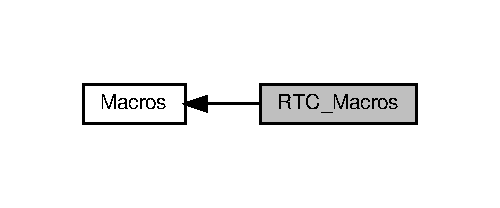
\includegraphics[width=240pt]{group___r_t_c___macros}
\end{center}
\end{figure}
\subsection*{Macros}
\begin{DoxyCompactItemize}
\item 
\mbox{\Hypertarget{group___r_t_c___macros_ga4e22feb6ffbc1cda32fadff5c740dc51}\label{group___r_t_c___macros_ga4e22feb6ffbc1cda32fadff5c740dc51}} 
\#define \hyperlink{group___r_t_c___macros_ga4e22feb6ffbc1cda32fadff5c740dc51}{R\+T\+C\+\_\+\+I\+RQ}~8
\begin{DoxyCompactList}\small\item\em R\+TC I\+RQ. \end{DoxyCompactList}\item 
\mbox{\Hypertarget{group___r_t_c___macros_ga710b98232df2c563009e6f8a6cd18220}\label{group___r_t_c___macros_ga710b98232df2c563009e6f8a6cd18220}} 
\#define \hyperlink{group___r_t_c___macros_ga710b98232df2c563009e6f8a6cd18220}{R\+T\+C\+\_\+\+A\+D\+D\+R\+\_\+\+R\+EG}~0x70
\begin{DoxyCompactList}\small\item\em R\+TC address register. \end{DoxyCompactList}\item 
\mbox{\Hypertarget{group___r_t_c___macros_ga2f258a00c59c3f347c8d2d4a75471ce0}\label{group___r_t_c___macros_ga2f258a00c59c3f347c8d2d4a75471ce0}} 
\#define \hyperlink{group___r_t_c___macros_ga2f258a00c59c3f347c8d2d4a75471ce0}{R\+T\+C\+\_\+\+D\+A\+T\+A\+\_\+\+R\+EG}~0x71
\begin{DoxyCompactList}\small\item\em R\+TC data register. \end{DoxyCompactList}\item 
\mbox{\Hypertarget{group___r_t_c___macros_gaa0e40d1cb9fea79e800aa79b8ca291f7}\label{group___r_t_c___macros_gaa0e40d1cb9fea79e800aa79b8ca291f7}} 
\#define \hyperlink{group___r_t_c___macros_gaa0e40d1cb9fea79e800aa79b8ca291f7}{R\+E\+G\+\_\+A}~0x0A
\begin{DoxyCompactList}\small\item\em Register A. \end{DoxyCompactList}\item 
\mbox{\Hypertarget{group___r_t_c___macros_ga28ed75c6727784e56c2bb8d828c876c9}\label{group___r_t_c___macros_ga28ed75c6727784e56c2bb8d828c876c9}} 
\#define \hyperlink{group___r_t_c___macros_ga28ed75c6727784e56c2bb8d828c876c9}{R\+E\+G\+\_\+B}~0x0B
\begin{DoxyCompactList}\small\item\em Register B. \end{DoxyCompactList}\item 
\mbox{\Hypertarget{group___r_t_c___macros_ga088e580de0961d5f30eb3366f97b324c}\label{group___r_t_c___macros_ga088e580de0961d5f30eb3366f97b324c}} 
\#define \hyperlink{group___r_t_c___macros_ga088e580de0961d5f30eb3366f97b324c}{R\+E\+G\+\_\+C}~0x0C
\begin{DoxyCompactList}\small\item\em Register C. \end{DoxyCompactList}\item 
\mbox{\Hypertarget{group___r_t_c___macros_ga8f2a2da8b96e20112d3f225636392424}\label{group___r_t_c___macros_ga8f2a2da8b96e20112d3f225636392424}} 
\#define \hyperlink{group___r_t_c___macros_ga8f2a2da8b96e20112d3f225636392424}{R\+E\+G\+\_\+D}~0x0D
\begin{DoxyCompactList}\small\item\em Register D. \end{DoxyCompactList}\item 
\mbox{\Hypertarget{group___r_t_c___macros_ga4d74cdb9a956c4f1783ad5aff00dc2b8}\label{group___r_t_c___macros_ga4d74cdb9a956c4f1783ad5aff00dc2b8}} 
\#define \hyperlink{group___r_t_c___macros_ga4d74cdb9a956c4f1783ad5aff00dc2b8}{R\+T\+C\+\_\+\+H\+O\+U\+RS}~0x04
\begin{DoxyCompactList}\small\item\em Register that stores the value of the hours. \end{DoxyCompactList}\item 
\mbox{\Hypertarget{group___r_t_c___macros_ga1bad17ef559ad960bba47fe87643b4c7}\label{group___r_t_c___macros_ga1bad17ef559ad960bba47fe87643b4c7}} 
\#define \hyperlink{group___r_t_c___macros_ga1bad17ef559ad960bba47fe87643b4c7}{R\+T\+C\+\_\+\+M\+I\+NS}~0x02
\begin{DoxyCompactList}\small\item\em Register that stores the value of the minutes. \end{DoxyCompactList}\item 
\mbox{\Hypertarget{group___r_t_c___macros_gaa86f159915dace411e5a7b74ecc130bd}\label{group___r_t_c___macros_gaa86f159915dace411e5a7b74ecc130bd}} 
\#define \hyperlink{group___r_t_c___macros_gaa86f159915dace411e5a7b74ecc130bd}{R\+T\+C\+\_\+\+S\+E\+CS}~0x00
\begin{DoxyCompactList}\small\item\em Register that stores the value of the seconds. \end{DoxyCompactList}\item 
\mbox{\Hypertarget{group___r_t_c___macros_ga8608b390793bacadc72dc418766b928b}\label{group___r_t_c___macros_ga8608b390793bacadc72dc418766b928b}} 
\#define \hyperlink{group___r_t_c___macros_ga8608b390793bacadc72dc418766b928b}{H\+O\+U\+R\+S\+\_\+\+A\+L\+A\+R\+M\+\_\+\+I\+N\+T\+E\+R\+R\+U\+PT}~B\+IT(5)
\begin{DoxyCompactList}\small\item\em Set to 1 if hours change. \end{DoxyCompactList}\item 
\mbox{\Hypertarget{group___r_t_c___macros_ga449a7797d3734eae1b1e9099f02b3e85}\label{group___r_t_c___macros_ga449a7797d3734eae1b1e9099f02b3e85}} 
\#define \hyperlink{group___r_t_c___macros_ga449a7797d3734eae1b1e9099f02b3e85}{M\+I\+N\+U\+T\+E\+S\+\_\+\+A\+L\+A\+R\+M\+\_\+\+I\+N\+T\+E\+R\+R\+U\+PT}~B\+IT(3)
\begin{DoxyCompactList}\small\item\em Set to 1 if minutes change. \end{DoxyCompactList}\end{DoxyCompactItemize}


\subsection{Detailed Description}
Macros of the R\+TC 
\hypertarget{group__main__functions}{}\section{Main\+\_\+functions}
\label{group__main__functions}\index{Main\+\_\+functions@{Main\+\_\+functions}}
\subsection*{Functions}
\begin{DoxyCompactItemize}
\item 
int \hyperlink{group__main__functions_ga230337632aac7d793969e926a66f0249}{timer\+\_\+manager} ()
\begin{DoxyCompactList}\small\item\em Function that calls the timer interrupt handler and manages all the timer related variables and functions. \end{DoxyCompactList}\item 
int \hyperlink{group__main__functions_gaaf064e0d3192ae8797d78dcb08bc838e}{keyboard\+\_\+manager} ()
\begin{DoxyCompactList}\small\item\em Function that calls the keyboard interrupt handler and manages all the keyboard related variables and functions. \end{DoxyCompactList}\item 
int \hyperlink{group__main__functions_ga8c9f11a032076f800d5d8e3faea17c9a}{mouse\+\_\+manager} ()
\begin{DoxyCompactList}\small\item\em Function that calls the mouse interrupt handler and manages all the mouse related variables and functions. \end{DoxyCompactList}\item 
int \hyperlink{group__main__functions_gac1cad6d7c8507831aa74d165972cb1a9}{rtc\+\_\+manager} ()
\begin{DoxyCompactList}\small\item\em Function that calls the R\+TC interrupt handler and manages all the R\+TC related variables and functions. \end{DoxyCompactList}\item 
void \hyperlink{group__main__functions_ga527ecae69a4a84b54c2c1e0fdfb4b72d}{draw\+\_\+clouds} (int jump\+\_\+counter)
\begin{DoxyCompactList}\small\item\em Function that works with the logic of the minigame. \end{DoxyCompactList}\end{DoxyCompactItemize}


\subsection{Detailed Description}
Main Functions of the Project 

\subsection{Function Documentation}
\mbox{\Hypertarget{group__main__functions_ga527ecae69a4a84b54c2c1e0fdfb4b72d}\label{group__main__functions_ga527ecae69a4a84b54c2c1e0fdfb4b72d}} 
\index{Main\+\_\+functions@{Main\+\_\+functions}!draw\+\_\+clouds@{draw\+\_\+clouds}}
\index{draw\+\_\+clouds@{draw\+\_\+clouds}!Main\+\_\+functions@{Main\+\_\+functions}}
\subsubsection{\texorpdfstring{draw\+\_\+clouds()}{draw\_clouds()}}
{\footnotesize\ttfamily void draw\+\_\+clouds (\begin{DoxyParamCaption}\item[{int}]{jump\+\_\+counter }\end{DoxyParamCaption})}



Function that works with the logic of the minigame. 

The clouds of the minigame change when the jump\+\_\+counter assumes different values


\begin{DoxyParams}{Parameters}
{\em jump\+\_\+counter} & variable used to help getting the score of the minigame and to use in the switch to decide wich cloud should be draw \\
\hline
\end{DoxyParams}
Here is the call graph for this function\+:\nopagebreak
\begin{figure}[H]
\begin{center}
\leavevmode
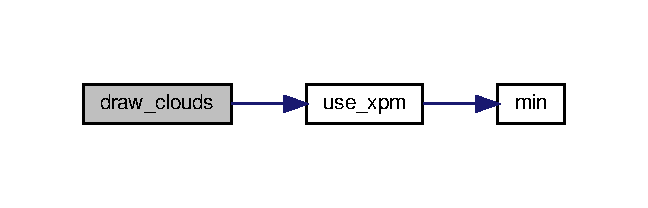
\includegraphics[width=311pt]{group__main__functions_ga527ecae69a4a84b54c2c1e0fdfb4b72d_cgraph}
\end{center}
\end{figure}
Here is the caller graph for this function\+:
\nopagebreak
\begin{figure}[H]
\begin{center}
\leavevmode
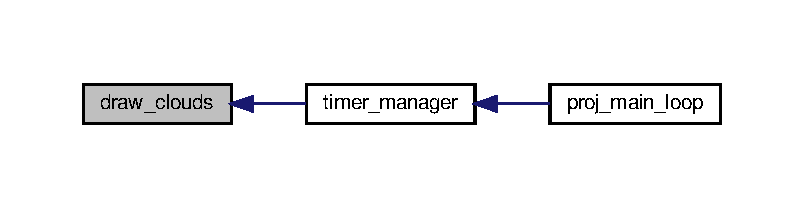
\includegraphics[width=350pt]{group__main__functions_ga527ecae69a4a84b54c2c1e0fdfb4b72d_icgraph}
\end{center}
\end{figure}
\mbox{\Hypertarget{group__main__functions_gaaf064e0d3192ae8797d78dcb08bc838e}\label{group__main__functions_gaaf064e0d3192ae8797d78dcb08bc838e}} 
\index{Main\+\_\+functions@{Main\+\_\+functions}!keyboard\+\_\+manager@{keyboard\+\_\+manager}}
\index{keyboard\+\_\+manager@{keyboard\+\_\+manager}!Main\+\_\+functions@{Main\+\_\+functions}}
\subsubsection{\texorpdfstring{keyboard\+\_\+manager()}{keyboard\_manager()}}
{\footnotesize\ttfamily int keyboard\+\_\+manager (\begin{DoxyParamCaption}{ }\end{DoxyParamCaption})}



Function that calls the keyboard interrupt handler and manages all the keyboard related variables and functions. 

\begin{DoxyReturn}{Returns}
Return 0 upon success 
\end{DoxyReturn}
Here is the call graph for this function\+:
\nopagebreak
\begin{figure}[H]
\begin{center}
\leavevmode
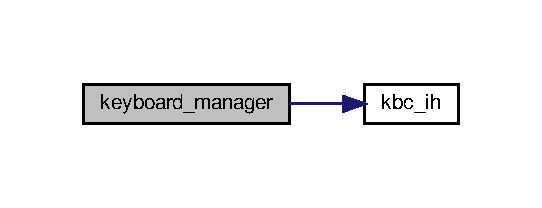
\includegraphics[width=260pt]{group__main__functions_gaaf064e0d3192ae8797d78dcb08bc838e_cgraph}
\end{center}
\end{figure}
Here is the caller graph for this function\+:\nopagebreak
\begin{figure}[H]
\begin{center}
\leavevmode
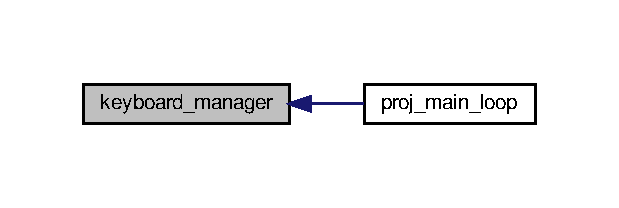
\includegraphics[width=297pt]{group__main__functions_gaaf064e0d3192ae8797d78dcb08bc838e_icgraph}
\end{center}
\end{figure}
\mbox{\Hypertarget{group__main__functions_ga8c9f11a032076f800d5d8e3faea17c9a}\label{group__main__functions_ga8c9f11a032076f800d5d8e3faea17c9a}} 
\index{Main\+\_\+functions@{Main\+\_\+functions}!mouse\+\_\+manager@{mouse\+\_\+manager}}
\index{mouse\+\_\+manager@{mouse\+\_\+manager}!Main\+\_\+functions@{Main\+\_\+functions}}
\subsubsection{\texorpdfstring{mouse\+\_\+manager()}{mouse\_manager()}}
{\footnotesize\ttfamily int mouse\+\_\+manager (\begin{DoxyParamCaption}{ }\end{DoxyParamCaption})}



Function that calls the mouse interrupt handler and manages all the mouse related variables and functions. 

\begin{DoxyReturn}{Returns}
Return 0 upon success 
\end{DoxyReturn}
Here is the call graph for this function\+:
\nopagebreak
\begin{figure}[H]
\begin{center}
\leavevmode
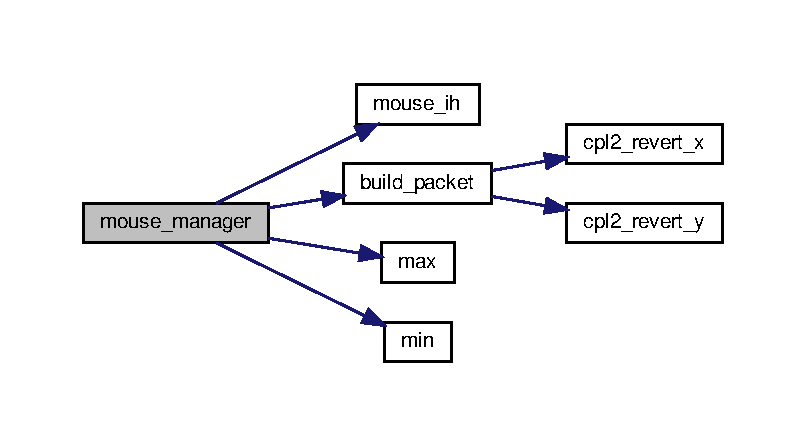
\includegraphics[width=350pt]{group__main__functions_ga8c9f11a032076f800d5d8e3faea17c9a_cgraph}
\end{center}
\end{figure}
Here is the caller graph for this function\+:\nopagebreak
\begin{figure}[H]
\begin{center}
\leavevmode
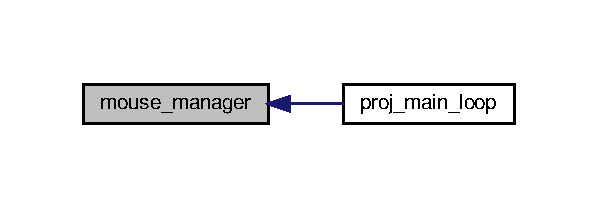
\includegraphics[width=287pt]{group__main__functions_ga8c9f11a032076f800d5d8e3faea17c9a_icgraph}
\end{center}
\end{figure}
\mbox{\Hypertarget{group__main__functions_gac1cad6d7c8507831aa74d165972cb1a9}\label{group__main__functions_gac1cad6d7c8507831aa74d165972cb1a9}} 
\index{Main\+\_\+functions@{Main\+\_\+functions}!rtc\+\_\+manager@{rtc\+\_\+manager}}
\index{rtc\+\_\+manager@{rtc\+\_\+manager}!Main\+\_\+functions@{Main\+\_\+functions}}
\subsubsection{\texorpdfstring{rtc\+\_\+manager()}{rtc\_manager()}}
{\footnotesize\ttfamily int rtc\+\_\+manager (\begin{DoxyParamCaption}{ }\end{DoxyParamCaption})}



Function that calls the R\+TC interrupt handler and manages all the R\+TC related variables and functions. 

\begin{DoxyReturn}{Returns}
Return 0 upon success 
\end{DoxyReturn}
Here is the call graph for this function\+:
\nopagebreak
\begin{figure}[H]
\begin{center}
\leavevmode
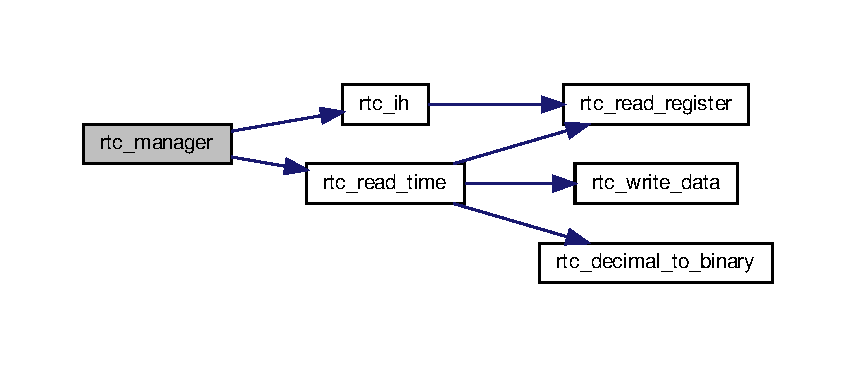
\includegraphics[width=350pt]{group__main__functions_gac1cad6d7c8507831aa74d165972cb1a9_cgraph}
\end{center}
\end{figure}
Here is the caller graph for this function\+:\nopagebreak
\begin{figure}[H]
\begin{center}
\leavevmode
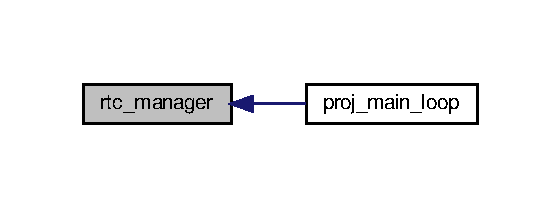
\includegraphics[width=269pt]{group__main__functions_gac1cad6d7c8507831aa74d165972cb1a9_icgraph}
\end{center}
\end{figure}
\mbox{\Hypertarget{group__main__functions_ga230337632aac7d793969e926a66f0249}\label{group__main__functions_ga230337632aac7d793969e926a66f0249}} 
\index{Main\+\_\+functions@{Main\+\_\+functions}!timer\+\_\+manager@{timer\+\_\+manager}}
\index{timer\+\_\+manager@{timer\+\_\+manager}!Main\+\_\+functions@{Main\+\_\+functions}}
\subsubsection{\texorpdfstring{timer\+\_\+manager()}{timer\_manager()}}
{\footnotesize\ttfamily int timer\+\_\+manager (\begin{DoxyParamCaption}{ }\end{DoxyParamCaption})}



Function that calls the timer interrupt handler and manages all the timer related variables and functions. 

\begin{DoxyReturn}{Returns}
Return 0 upon success 
\end{DoxyReturn}
Here is the call graph for this function\+:
\nopagebreak
\begin{figure}[H]
\begin{center}
\leavevmode
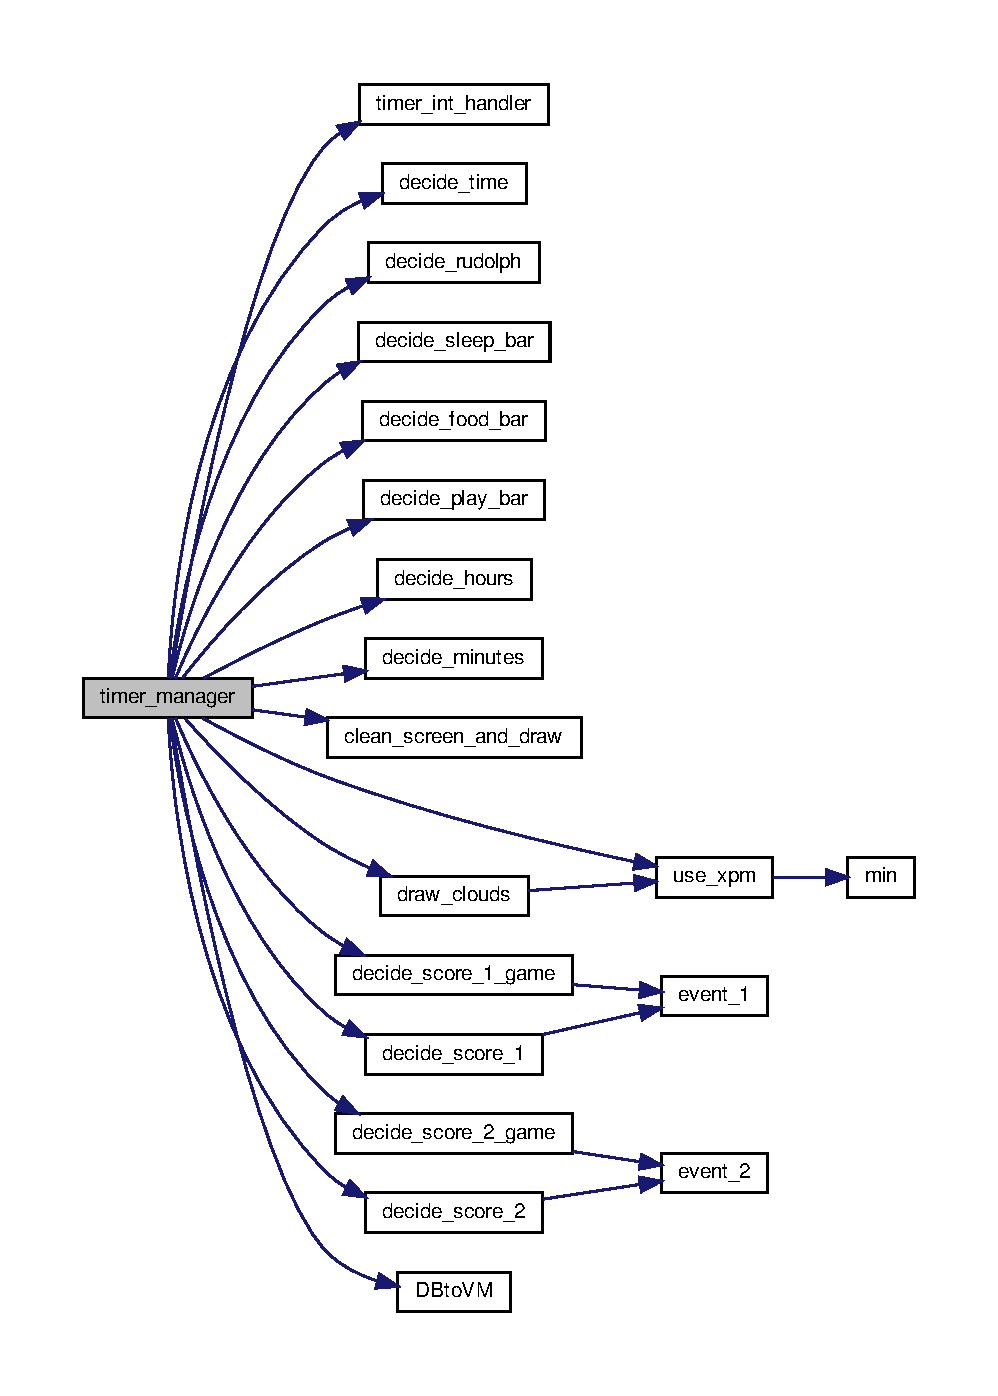
\includegraphics[width=350pt]{group__main__functions_ga230337632aac7d793969e926a66f0249_cgraph}
\end{center}
\end{figure}
Here is the caller graph for this function\+:\nopagebreak
\begin{figure}[H]
\begin{center}
\leavevmode
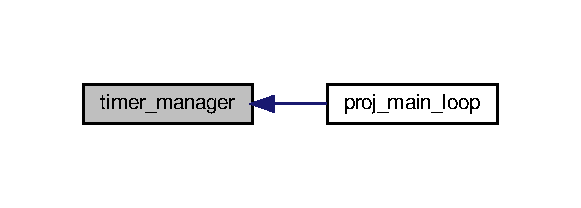
\includegraphics[width=279pt]{group__main__functions_ga230337632aac7d793969e926a66f0249_icgraph}
\end{center}
\end{figure}

\hypertarget{group__mouse}{}\section{Mouse}
\label{group__mouse}\index{Mouse@{Mouse}}
\subsection*{Functions}
\begin{DoxyCompactItemize}
\item 
uint16\+\_\+t \hyperlink{group__mouse_gaca472150bedc1bf9e0008ffd9929b165}{cpl2\+\_\+revert\+\_\+x} (uint8\+\_\+t byte)
\begin{DoxyCompactList}\small\item\em Function that reverts the cpl2 value of the byte\mbox{[}1\mbox{]} (x\+Delta) of the mouse packet. \end{DoxyCompactList}\item 
uint16\+\_\+t \hyperlink{group__mouse_gaf9b79deb06853057db6850cb4b7ec917}{cpl2\+\_\+revert\+\_\+y} (uint8\+\_\+t byte)
\begin{DoxyCompactList}\small\item\em Function that reverts the cpl2 value of the byte\mbox{[}2\mbox{]} (Y\+Delta) of the mouse packet. \end{DoxyCompactList}\item 
void \hyperlink{group__mouse_ga7d38d68c1222c116e819346c1c3d36f1}{build\+\_\+packet} (struct packet $\ast$pack)
\begin{DoxyCompactList}\small\item\em Function that builds a mouse packet. \end{DoxyCompactList}\item 
int \hyperlink{group__mouse_ga9da18257ff113b686bb826d154bfaa87}{mouse\+\_\+subscribe\+\_\+int} (uint8\+\_\+t $\ast$bit\+\_\+no)
\begin{DoxyCompactList}\small\item\em Function that subscribes mouse interruptions. \end{DoxyCompactList}\item 
int \hyperlink{group__mouse_ga685ad2706aca36d9869a30a19b9f446a}{mouse\+\_\+unsubscribe\+\_\+int} ()
\begin{DoxyCompactList}\small\item\em Function that unsubscribes mouse interruptions. \end{DoxyCompactList}\item 
\mbox{\Hypertarget{group__mouse_ga210374b50462acdedab00df64d5cea3c}\label{group__mouse_ga210374b50462acdedab00df64d5cea3c}} 
void() \hyperlink{group__mouse_ga210374b50462acdedab00df64d5cea3c}{mouse\+\_\+ih} ()
\begin{DoxyCompactList}\small\item\em Mouse interrupt handler. \end{DoxyCompactList}\item 
int() \hyperlink{group__mouse_ga7e311379d4d64f88873ef8ade5c82a25}{mouse\+\_\+disable\+\_\+data\+\_\+reporting} ()
\begin{DoxyCompactList}\small\item\em Function that disables the mouse data reporting. \end{DoxyCompactList}\item 
int() \hyperlink{group__mouse_ga90562ec8e969e4014d728adb0fc91e31}{mouse\+\_\+enable\+\_\+datarp} ()
\begin{DoxyCompactList}\small\item\em Function that enables the mouse data reporting. \end{DoxyCompactList}\item 
int() \hyperlink{group__mouse_ga926121b9c6d89ac8825f115e3eb8dac3}{send\+\_\+command} (uint8\+\_\+t command)
\begin{DoxyCompactList}\small\item\em Function that saves a command in the keyboard command register. \end{DoxyCompactList}\item 
int() \hyperlink{group__mouse_ga4f9755f5c9975e9b13daa3e34f26f5cf}{write\+\_\+argument} (uint8\+\_\+t argument)
\begin{DoxyCompactList}\small\item\em Function that writes an argument in the output buffer. \end{DoxyCompactList}\item 
int() \hyperlink{group__mouse_ga58c043049bb31ec7bad65594a8341a5d}{set\+\_\+stream\+\_\+mode} ()
\begin{DoxyCompactList}\small\item\em Function that sets the stream mode. \end{DoxyCompactList}\item 
int() \hyperlink{group__mouse_gad25b8bf71166026dbf192c6d013d54d6}{read\+\_\+data} ()
\begin{DoxyCompactList}\small\item\em Function that sends a command to read data from the mouse. \end{DoxyCompactList}\end{DoxyCompactItemize}


\subsection{Detailed Description}
mouse main functions 

\subsection{Function Documentation}
\mbox{\Hypertarget{group__mouse_ga7d38d68c1222c116e819346c1c3d36f1}\label{group__mouse_ga7d38d68c1222c116e819346c1c3d36f1}} 
\index{Mouse@{Mouse}!build\+\_\+packet@{build\+\_\+packet}}
\index{build\+\_\+packet@{build\+\_\+packet}!Mouse@{Mouse}}
\subsubsection{\texorpdfstring{build\+\_\+packet()}{build\_packet()}}
{\footnotesize\ttfamily void build\+\_\+packet (\begin{DoxyParamCaption}\item[{struct packet $\ast$}]{pack }\end{DoxyParamCaption})}



Function that builds a mouse packet. 


\begin{DoxyParams}{Parameters}
{\em pack} & pointer to a struct packet of the mouse packet that is gonna be built \\
\hline
\end{DoxyParams}
Here is the call graph for this function\+:\nopagebreak
\begin{figure}[H]
\begin{center}
\leavevmode
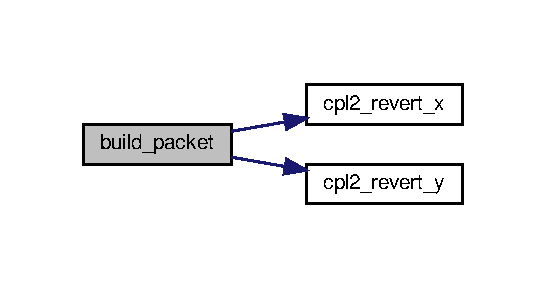
\includegraphics[width=262pt]{group__mouse_ga7d38d68c1222c116e819346c1c3d36f1_cgraph}
\end{center}
\end{figure}
Here is the caller graph for this function\+:
\nopagebreak
\begin{figure}[H]
\begin{center}
\leavevmode
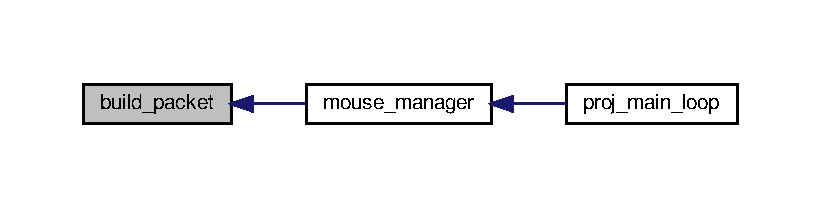
\includegraphics[width=350pt]{group__mouse_ga7d38d68c1222c116e819346c1c3d36f1_icgraph}
\end{center}
\end{figure}
\mbox{\Hypertarget{group__mouse_gaca472150bedc1bf9e0008ffd9929b165}\label{group__mouse_gaca472150bedc1bf9e0008ffd9929b165}} 
\index{Mouse@{Mouse}!cpl2\+\_\+revert\+\_\+x@{cpl2\+\_\+revert\+\_\+x}}
\index{cpl2\+\_\+revert\+\_\+x@{cpl2\+\_\+revert\+\_\+x}!Mouse@{Mouse}}
\subsubsection{\texorpdfstring{cpl2\+\_\+revert\+\_\+x()}{cpl2\_revert\_x()}}
{\footnotesize\ttfamily uint16\+\_\+t cpl2\+\_\+revert\+\_\+x (\begin{DoxyParamCaption}\item[{uint8\+\_\+t}]{byte }\end{DoxyParamCaption})}



Function that reverts the cpl2 value of the byte\mbox{[}1\mbox{]} (x\+Delta) of the mouse packet. 


\begin{DoxyParams}{Parameters}
{\em byte} & byte\mbox{[}1\mbox{]} of the mouse packet\\
\hline
\end{DoxyParams}
\begin{DoxyReturn}{Returns}
Returns the new value of the byte 
\end{DoxyReturn}
Here is the caller graph for this function\+:
\nopagebreak
\begin{figure}[H]
\begin{center}
\leavevmode
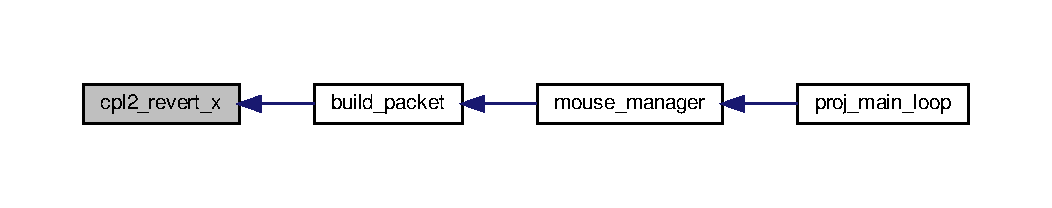
\includegraphics[width=350pt]{group__mouse_gaca472150bedc1bf9e0008ffd9929b165_icgraph}
\end{center}
\end{figure}
\mbox{\Hypertarget{group__mouse_gaf9b79deb06853057db6850cb4b7ec917}\label{group__mouse_gaf9b79deb06853057db6850cb4b7ec917}} 
\index{Mouse@{Mouse}!cpl2\+\_\+revert\+\_\+y@{cpl2\+\_\+revert\+\_\+y}}
\index{cpl2\+\_\+revert\+\_\+y@{cpl2\+\_\+revert\+\_\+y}!Mouse@{Mouse}}
\subsubsection{\texorpdfstring{cpl2\+\_\+revert\+\_\+y()}{cpl2\_revert\_y()}}
{\footnotesize\ttfamily uint16\+\_\+t cpl2\+\_\+revert\+\_\+y (\begin{DoxyParamCaption}\item[{uint8\+\_\+t}]{byte }\end{DoxyParamCaption})}



Function that reverts the cpl2 value of the byte\mbox{[}2\mbox{]} (Y\+Delta) of the mouse packet. 


\begin{DoxyParams}{Parameters}
{\em byte} & byte\mbox{[}2\mbox{]} of the mouse packet\\
\hline
\end{DoxyParams}
\begin{DoxyReturn}{Returns}
Returns the new value of the byte 
\end{DoxyReturn}
Here is the caller graph for this function\+:
\nopagebreak
\begin{figure}[H]
\begin{center}
\leavevmode
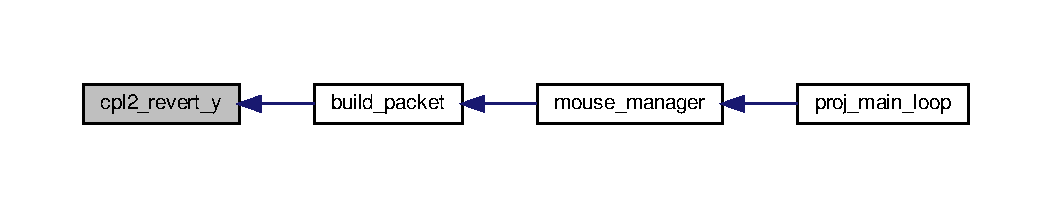
\includegraphics[width=350pt]{group__mouse_gaf9b79deb06853057db6850cb4b7ec917_icgraph}
\end{center}
\end{figure}
\mbox{\Hypertarget{group__mouse_ga7e311379d4d64f88873ef8ade5c82a25}\label{group__mouse_ga7e311379d4d64f88873ef8ade5c82a25}} 
\index{Mouse@{Mouse}!mouse\+\_\+disable\+\_\+data\+\_\+reporting@{mouse\+\_\+disable\+\_\+data\+\_\+reporting}}
\index{mouse\+\_\+disable\+\_\+data\+\_\+reporting@{mouse\+\_\+disable\+\_\+data\+\_\+reporting}!Mouse@{Mouse}}
\subsubsection{\texorpdfstring{mouse\+\_\+disable\+\_\+data\+\_\+reporting()}{mouse\_disable\_data\_reporting()}}
{\footnotesize\ttfamily int() mouse\+\_\+disable\+\_\+data\+\_\+reporting (\begin{DoxyParamCaption}{ }\end{DoxyParamCaption})}



Function that disables the mouse data reporting. 

\begin{DoxyReturn}{Returns}
Returns 0 upon success 
\end{DoxyReturn}
Here is the call graph for this function\+:
\nopagebreak
\begin{figure}[H]
\begin{center}
\leavevmode
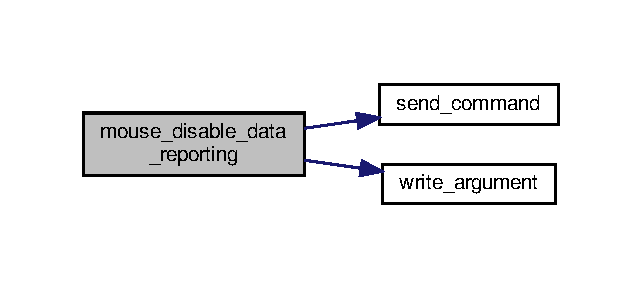
\includegraphics[width=308pt]{group__mouse_ga7e311379d4d64f88873ef8ade5c82a25_cgraph}
\end{center}
\end{figure}
Here is the caller graph for this function\+:\nopagebreak
\begin{figure}[H]
\begin{center}
\leavevmode
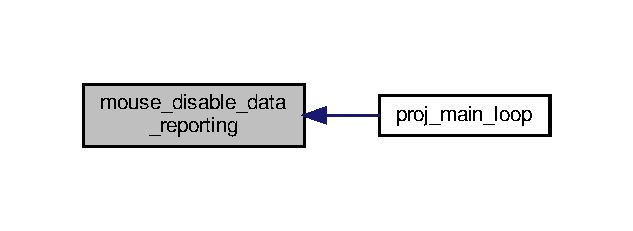
\includegraphics[width=304pt]{group__mouse_ga7e311379d4d64f88873ef8ade5c82a25_icgraph}
\end{center}
\end{figure}
\mbox{\Hypertarget{group__mouse_ga90562ec8e969e4014d728adb0fc91e31}\label{group__mouse_ga90562ec8e969e4014d728adb0fc91e31}} 
\index{Mouse@{Mouse}!mouse\+\_\+enable\+\_\+datarp@{mouse\+\_\+enable\+\_\+datarp}}
\index{mouse\+\_\+enable\+\_\+datarp@{mouse\+\_\+enable\+\_\+datarp}!Mouse@{Mouse}}
\subsubsection{\texorpdfstring{mouse\+\_\+enable\+\_\+datarp()}{mouse\_enable\_datarp()}}
{\footnotesize\ttfamily int() mouse\+\_\+enable\+\_\+datarp (\begin{DoxyParamCaption}{ }\end{DoxyParamCaption})}



Function that enables the mouse data reporting. 

\begin{DoxyReturn}{Returns}
Returns 0 upon success 
\end{DoxyReturn}
Here is the call graph for this function\+:
\nopagebreak
\begin{figure}[H]
\begin{center}
\leavevmode
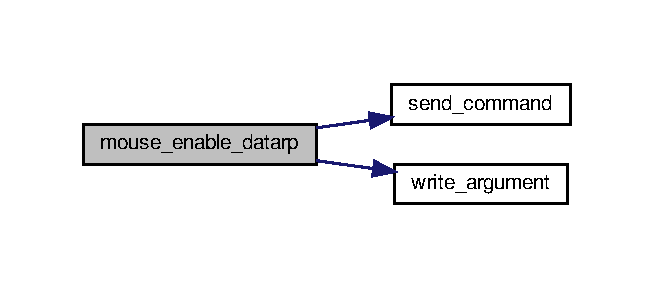
\includegraphics[width=314pt]{group__mouse_ga90562ec8e969e4014d728adb0fc91e31_cgraph}
\end{center}
\end{figure}
\mbox{\Hypertarget{group__mouse_ga9da18257ff113b686bb826d154bfaa87}\label{group__mouse_ga9da18257ff113b686bb826d154bfaa87}} 
\index{Mouse@{Mouse}!mouse\+\_\+subscribe\+\_\+int@{mouse\+\_\+subscribe\+\_\+int}}
\index{mouse\+\_\+subscribe\+\_\+int@{mouse\+\_\+subscribe\+\_\+int}!Mouse@{Mouse}}
\subsubsection{\texorpdfstring{mouse\+\_\+subscribe\+\_\+int()}{mouse\_subscribe\_int()}}
{\footnotesize\ttfamily int mouse\+\_\+subscribe\+\_\+int (\begin{DoxyParamCaption}\item[{uint8\+\_\+t $\ast$}]{bit\+\_\+no }\end{DoxyParamCaption})}



Function that subscribes mouse interruptions. 

\begin{DoxyReturn}{Returns}
Return 0 upon success 
\end{DoxyReturn}
Here is the caller graph for this function\+:\nopagebreak
\begin{figure}[H]
\begin{center}
\leavevmode
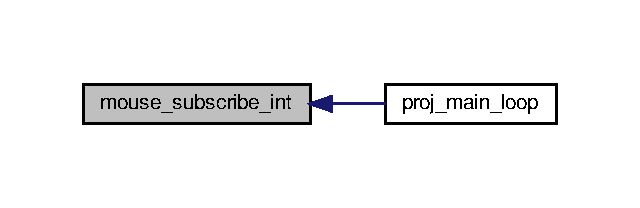
\includegraphics[width=307pt]{group__mouse_ga9da18257ff113b686bb826d154bfaa87_icgraph}
\end{center}
\end{figure}
\mbox{\Hypertarget{group__mouse_ga685ad2706aca36d9869a30a19b9f446a}\label{group__mouse_ga685ad2706aca36d9869a30a19b9f446a}} 
\index{Mouse@{Mouse}!mouse\+\_\+unsubscribe\+\_\+int@{mouse\+\_\+unsubscribe\+\_\+int}}
\index{mouse\+\_\+unsubscribe\+\_\+int@{mouse\+\_\+unsubscribe\+\_\+int}!Mouse@{Mouse}}
\subsubsection{\texorpdfstring{mouse\+\_\+unsubscribe\+\_\+int()}{mouse\_unsubscribe\_int()}}
{\footnotesize\ttfamily int mouse\+\_\+unsubscribe\+\_\+int (\begin{DoxyParamCaption}{ }\end{DoxyParamCaption})}



Function that unsubscribes mouse interruptions. 

\begin{DoxyReturn}{Returns}
Return 0 upon success 
\end{DoxyReturn}
Here is the caller graph for this function\+:\nopagebreak
\begin{figure}[H]
\begin{center}
\leavevmode
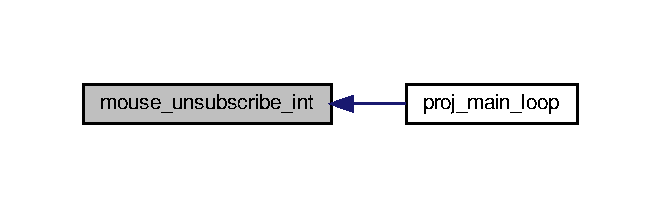
\includegraphics[width=317pt]{group__mouse_ga685ad2706aca36d9869a30a19b9f446a_icgraph}
\end{center}
\end{figure}
\mbox{\Hypertarget{group__mouse_gad25b8bf71166026dbf192c6d013d54d6}\label{group__mouse_gad25b8bf71166026dbf192c6d013d54d6}} 
\index{Mouse@{Mouse}!read\+\_\+data@{read\+\_\+data}}
\index{read\+\_\+data@{read\+\_\+data}!Mouse@{Mouse}}
\subsubsection{\texorpdfstring{read\+\_\+data()}{read\_data()}}
{\footnotesize\ttfamily int() read\+\_\+data (\begin{DoxyParamCaption}{ }\end{DoxyParamCaption})}



Function that sends a command to read data from the mouse. 

\begin{DoxyReturn}{Returns}
Returns 0 upon success 
\end{DoxyReturn}
Here is the call graph for this function\+:
\nopagebreak
\begin{figure}[H]
\begin{center}
\leavevmode
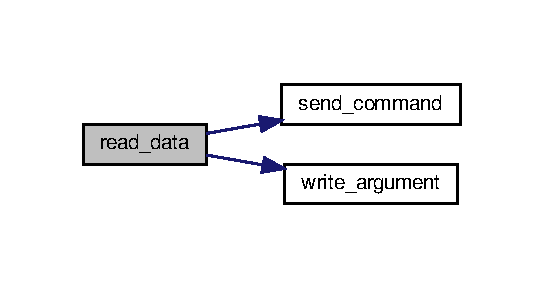
\includegraphics[width=261pt]{group__mouse_gad25b8bf71166026dbf192c6d013d54d6_cgraph}
\end{center}
\end{figure}
\mbox{\Hypertarget{group__mouse_ga926121b9c6d89ac8825f115e3eb8dac3}\label{group__mouse_ga926121b9c6d89ac8825f115e3eb8dac3}} 
\index{Mouse@{Mouse}!send\+\_\+command@{send\+\_\+command}}
\index{send\+\_\+command@{send\+\_\+command}!Mouse@{Mouse}}
\subsubsection{\texorpdfstring{send\+\_\+command()}{send\_command()}}
{\footnotesize\ttfamily int() send\+\_\+command (\begin{DoxyParamCaption}\item[{uint8\+\_\+t}]{command }\end{DoxyParamCaption})}



Function that saves a command in the keyboard command register. 


\begin{DoxyParams}{Parameters}
{\em command} & command that is gonna be saved\\
\hline
\end{DoxyParams}
\begin{DoxyReturn}{Returns}
Returns 0 upon success 
\end{DoxyReturn}
Here is the caller graph for this function\+:
\nopagebreak
\begin{figure}[H]
\begin{center}
\leavevmode
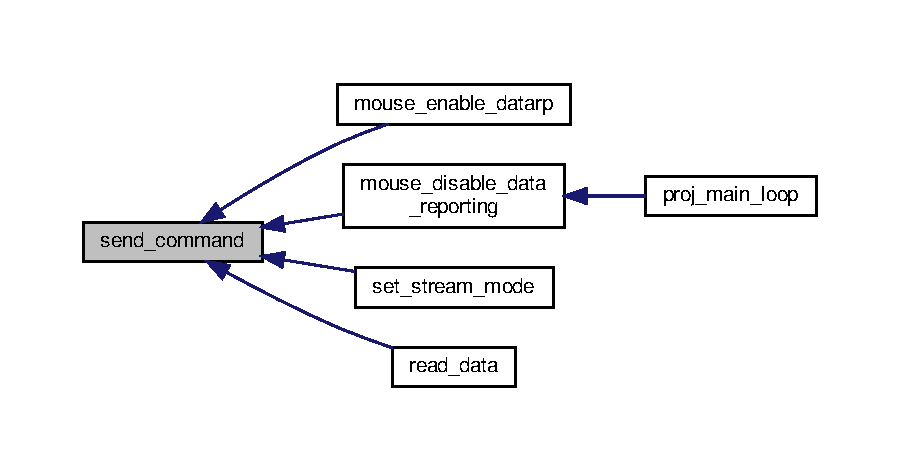
\includegraphics[width=350pt]{group__mouse_ga926121b9c6d89ac8825f115e3eb8dac3_icgraph}
\end{center}
\end{figure}
\mbox{\Hypertarget{group__mouse_ga58c043049bb31ec7bad65594a8341a5d}\label{group__mouse_ga58c043049bb31ec7bad65594a8341a5d}} 
\index{Mouse@{Mouse}!set\+\_\+stream\+\_\+mode@{set\+\_\+stream\+\_\+mode}}
\index{set\+\_\+stream\+\_\+mode@{set\+\_\+stream\+\_\+mode}!Mouse@{Mouse}}
\subsubsection{\texorpdfstring{set\+\_\+stream\+\_\+mode()}{set\_stream\_mode()}}
{\footnotesize\ttfamily int() set\+\_\+stream\+\_\+mode (\begin{DoxyParamCaption}{ }\end{DoxyParamCaption})}



Function that sets the stream mode. 

\begin{DoxyReturn}{Returns}
Returns 0 upon success 
\end{DoxyReturn}
Here is the call graph for this function\+:
\nopagebreak
\begin{figure}[H]
\begin{center}
\leavevmode
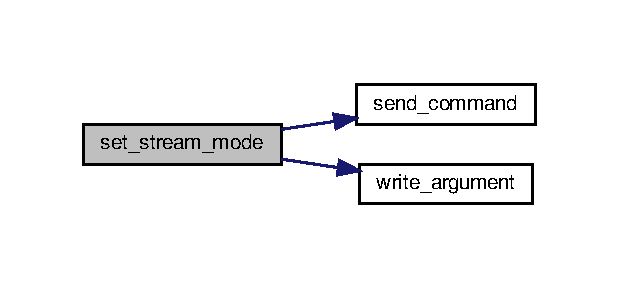
\includegraphics[width=297pt]{group__mouse_ga58c043049bb31ec7bad65594a8341a5d_cgraph}
\end{center}
\end{figure}
\mbox{\Hypertarget{group__mouse_ga4f9755f5c9975e9b13daa3e34f26f5cf}\label{group__mouse_ga4f9755f5c9975e9b13daa3e34f26f5cf}} 
\index{Mouse@{Mouse}!write\+\_\+argument@{write\+\_\+argument}}
\index{write\+\_\+argument@{write\+\_\+argument}!Mouse@{Mouse}}
\subsubsection{\texorpdfstring{write\+\_\+argument()}{write\_argument()}}
{\footnotesize\ttfamily int() write\+\_\+argument (\begin{DoxyParamCaption}\item[{uint8\+\_\+t}]{argument }\end{DoxyParamCaption})}



Function that writes an argument in the output buffer. 


\begin{DoxyParams}{Parameters}
{\em argument} & command that is gonna be written\\
\hline
\end{DoxyParams}
\begin{DoxyReturn}{Returns}
Returns 0 upon success 
\end{DoxyReturn}
Here is the caller graph for this function\+:
\nopagebreak
\begin{figure}[H]
\begin{center}
\leavevmode
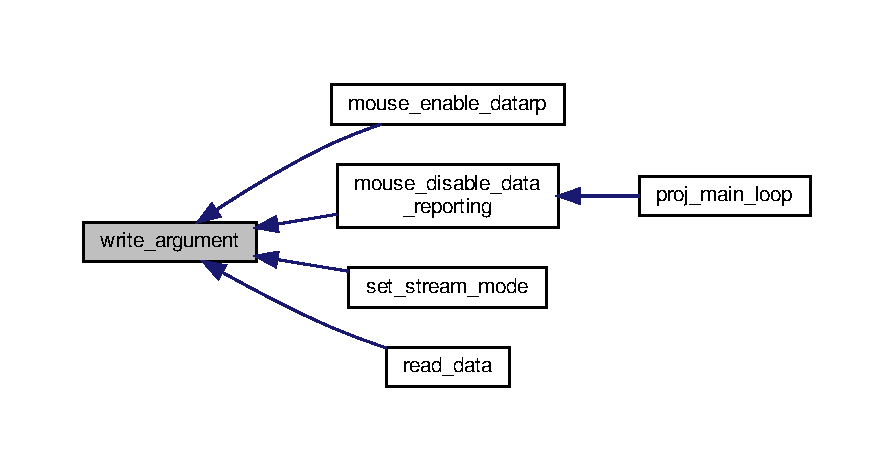
\includegraphics[width=350pt]{group__mouse_ga4f9755f5c9975e9b13daa3e34f26f5cf_icgraph}
\end{center}
\end{figure}

\hypertarget{group__myutils}{}\section{Myutils}
\label{group__myutils}\index{Myutils@{Myutils}}
\subsection*{Functions}
\begin{DoxyCompactItemize}
\item 
int32\+\_\+t \hyperlink{group__myutils_ga86fabf639ab773666d2c7936b104a668}{min} (int32\+\_\+t a, int32\+\_\+t b)
\begin{DoxyCompactList}\small\item\em Function that gets the smallest of 2 numbers. \end{DoxyCompactList}\item 
int32\+\_\+t \hyperlink{group__myutils_gad2cb7db3e303727f643020a668377947}{max} (int32\+\_\+t a, int32\+\_\+t b)
\begin{DoxyCompactList}\small\item\em Function that gets the bigger of 2 numbers. \end{DoxyCompactList}\end{DoxyCompactItemize}


\subsection{Detailed Description}
some functions 

\subsection{Function Documentation}
\mbox{\Hypertarget{group__myutils_gad2cb7db3e303727f643020a668377947}\label{group__myutils_gad2cb7db3e303727f643020a668377947}} 
\index{Myutils@{Myutils}!max@{max}}
\index{max@{max}!Myutils@{Myutils}}
\subsubsection{\texorpdfstring{max()}{max()}}
{\footnotesize\ttfamily int32\+\_\+t max (\begin{DoxyParamCaption}\item[{int32\+\_\+t}]{a,  }\item[{int32\+\_\+t}]{b }\end{DoxyParamCaption})}



Function that gets the bigger of 2 numbers. 


\begin{DoxyParams}{Parameters}
{\em a} & one of the numbers that is being compared \\
\hline
{\em b} & the other number that is being compared\\
\hline
\end{DoxyParams}
\begin{DoxyReturn}{Returns}
Return the bigger number 
\end{DoxyReturn}
Here is the caller graph for this function\+:
\nopagebreak
\begin{figure}[H]
\begin{center}
\leavevmode
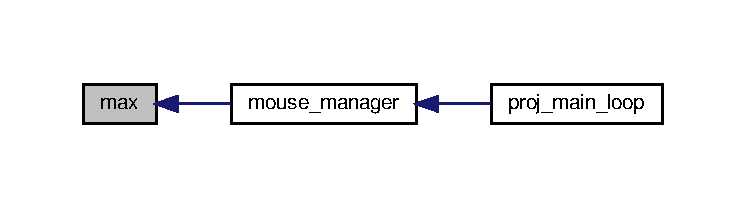
\includegraphics[width=350pt]{group__myutils_gad2cb7db3e303727f643020a668377947_icgraph}
\end{center}
\end{figure}
\mbox{\Hypertarget{group__myutils_ga86fabf639ab773666d2c7936b104a668}\label{group__myutils_ga86fabf639ab773666d2c7936b104a668}} 
\index{Myutils@{Myutils}!min@{min}}
\index{min@{min}!Myutils@{Myutils}}
\subsubsection{\texorpdfstring{min()}{min()}}
{\footnotesize\ttfamily int32\+\_\+t min (\begin{DoxyParamCaption}\item[{int32\+\_\+t}]{a,  }\item[{int32\+\_\+t}]{b }\end{DoxyParamCaption})}



Function that gets the smallest of 2 numbers. 


\begin{DoxyParams}{Parameters}
{\em a} & one of the numbers that is being compared \\
\hline
{\em b} & the other number that is being compared\\
\hline
\end{DoxyParams}
\begin{DoxyReturn}{Returns}
Return the smallest number 
\end{DoxyReturn}
Here is the caller graph for this function\+:
\nopagebreak
\begin{figure}[H]
\begin{center}
\leavevmode
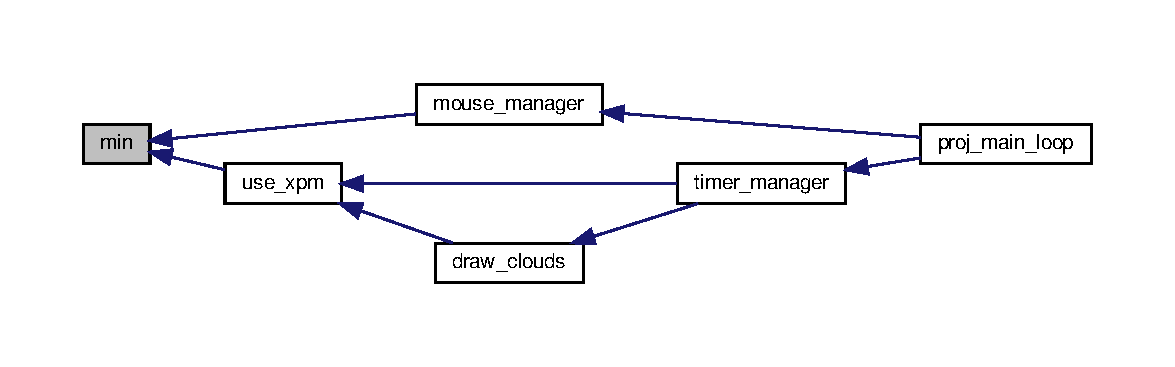
\includegraphics[width=350pt]{group__myutils_ga86fabf639ab773666d2c7936b104a668_icgraph}
\end{center}
\end{figure}

\hypertarget{group__main__loop}{}\section{Main\+\_\+loop}
\label{group__main__loop}\index{Main\+\_\+loop@{Main\+\_\+loop}}
\subsection*{Functions}
\begin{DoxyCompactItemize}
\item 
int() \hyperlink{group__main__loop_ga2a16f651eccbd248e1ad3b3b924b143b}{proj\+\_\+main\+\_\+loop} (int argc, char $\ast$argv\mbox{[}$\,$\mbox{]})
\begin{DoxyCompactList}\small\item\em Main loop of the project. \end{DoxyCompactList}\end{DoxyCompactItemize}


\subsection{Detailed Description}
Main\+\_\+loop of the project 

\subsection{Function Documentation}
\mbox{\Hypertarget{group__main__loop_ga2a16f651eccbd248e1ad3b3b924b143b}\label{group__main__loop_ga2a16f651eccbd248e1ad3b3b924b143b}} 
\index{Main\+\_\+loop@{Main\+\_\+loop}!proj\+\_\+main\+\_\+loop@{proj\+\_\+main\+\_\+loop}}
\index{proj\+\_\+main\+\_\+loop@{proj\+\_\+main\+\_\+loop}!Main\+\_\+loop@{Main\+\_\+loop}}
\subsubsection{\texorpdfstring{proj\+\_\+main\+\_\+loop()}{proj\_main\_loop()}}
{\footnotesize\ttfamily int() proj\+\_\+main\+\_\+loop (\begin{DoxyParamCaption}\item[{int}]{argc,  }\item[{char $\ast$}]{argv\mbox{[}$\,$\mbox{]} }\end{DoxyParamCaption})}



Main loop of the project. 

Driver Receive loop

\begin{DoxyReturn}{Returns}
Return 0 upon success 
\end{DoxyReturn}
Here is the call graph for this function\+:\nopagebreak
\begin{figure}[H]
\begin{center}
\leavevmode
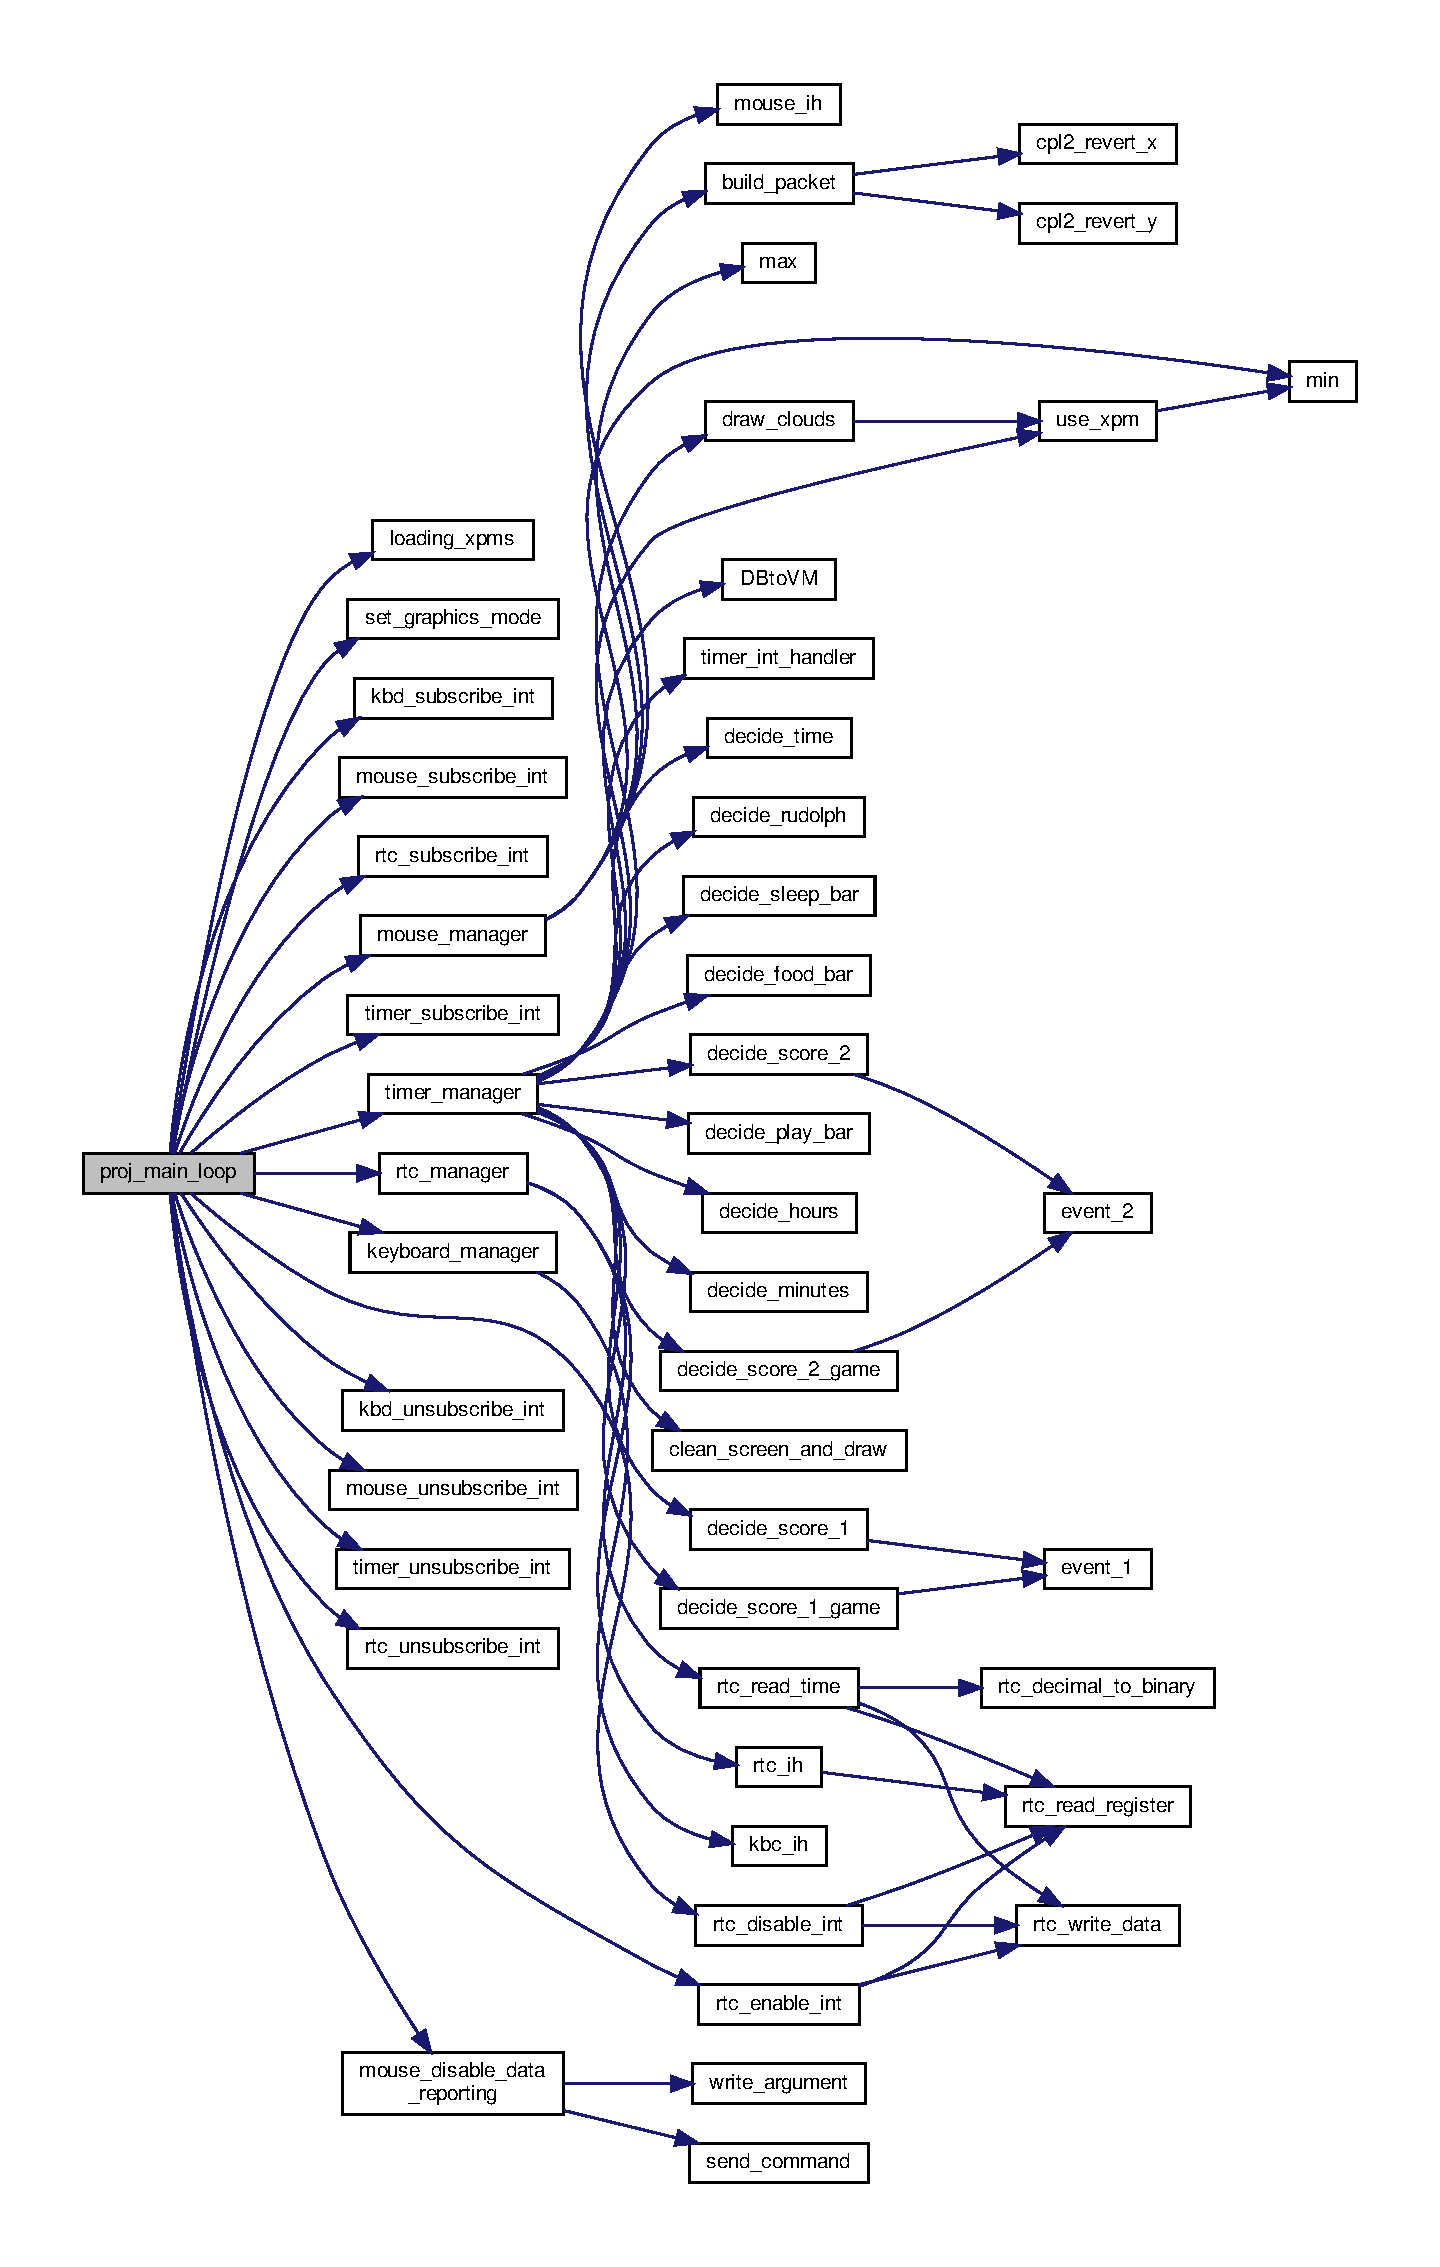
\includegraphics[height=550pt]{group__main__loop_ga2a16f651eccbd248e1ad3b3b924b143b_cgraph}
\end{center}
\end{figure}

\hypertarget{group__mouse__macros}{}\section{Mouse\+\_\+macros}
\label{group__mouse__macros}\index{Mouse\+\_\+macros@{Mouse\+\_\+macros}}
\subsection*{Macros}
\begin{DoxyCompactItemize}
\item 
\mbox{\Hypertarget{group__mouse__macros_ga45967c9e25447ba853cf6fb4ac545fe6}\label{group__mouse__macros_ga45967c9e25447ba853cf6fb4ac545fe6}} 
\#define \hyperlink{group__mouse__macros_ga45967c9e25447ba853cf6fb4ac545fe6}{O\+BF}~0x01
\begin{DoxyCompactList}\small\item\em status register bit 0 \end{DoxyCompactList}\item 
\mbox{\Hypertarget{group__mouse__macros_ga307ab71673e26ec42b28a3bca05d4cb5}\label{group__mouse__macros_ga307ab71673e26ec42b28a3bca05d4cb5}} 
\#define \hyperlink{group__mouse__macros_ga307ab71673e26ec42b28a3bca05d4cb5}{P\+A\+R\+\_\+\+E\+RR}~0x80
\begin{DoxyCompactList}\small\item\em status register bit 7 \end{DoxyCompactList}\item 
\mbox{\Hypertarget{group__mouse__macros_ga45ba202b05caf39795aeca91b0ae547e}\label{group__mouse__macros_ga45ba202b05caf39795aeca91b0ae547e}} 
\#define \hyperlink{group__mouse__macros_ga45ba202b05caf39795aeca91b0ae547e}{T\+I\+M\+E\+O\+UT}~0x40
\begin{DoxyCompactList}\small\item\em status register bit 6 \end{DoxyCompactList}\item 
\mbox{\Hypertarget{group__mouse__macros_ga1b41fd2be63532d4ab910f8b256c3811}\label{group__mouse__macros_ga1b41fd2be63532d4ab910f8b256c3811}} 
\#define \hyperlink{group__mouse__macros_ga1b41fd2be63532d4ab910f8b256c3811}{A\+UX}~0x20
\begin{DoxyCompactList}\small\item\em status register bit 5 \end{DoxyCompactList}\item 
\mbox{\Hypertarget{group__mouse__macros_ga03f542f1e0e2ba512c4ed189decfee3d}\label{group__mouse__macros_ga03f542f1e0e2ba512c4ed189decfee3d}} 
\#define \hyperlink{group__mouse__macros_ga03f542f1e0e2ba512c4ed189decfee3d}{I\+NH}~0x10
\begin{DoxyCompactList}\small\item\em status register bit 4 \end{DoxyCompactList}\item 
\mbox{\Hypertarget{group__mouse__macros_ga2946bc30423c2a996eeafa49e995c30e}\label{group__mouse__macros_ga2946bc30423c2a996eeafa49e995c30e}} 
\#define \hyperlink{group__mouse__macros_ga2946bc30423c2a996eeafa49e995c30e}{A2}~0x08
\begin{DoxyCompactList}\small\item\em status register bit 3 \end{DoxyCompactList}\item 
\mbox{\Hypertarget{group__mouse__macros_gae3d9f52a1a315303ad04f0576bd42a25}\label{group__mouse__macros_gae3d9f52a1a315303ad04f0576bd42a25}} 
\#define \hyperlink{group__mouse__macros_gae3d9f52a1a315303ad04f0576bd42a25}{S\+YS}~0x04
\begin{DoxyCompactList}\small\item\em status register bit 2 \end{DoxyCompactList}\item 
\mbox{\Hypertarget{group__mouse__macros_ga3c48b10907056351582baf9f6478598e}\label{group__mouse__macros_ga3c48b10907056351582baf9f6478598e}} 
\#define \hyperlink{group__mouse__macros_ga3c48b10907056351582baf9f6478598e}{I\+BF}~0x02
\begin{DoxyCompactList}\small\item\em status register bit 1 \end{DoxyCompactList}\item 
\mbox{\Hypertarget{group__mouse__macros_ga85964cb90343bb1a029b1d1b4229f910}\label{group__mouse__macros_ga85964cb90343bb1a029b1d1b4229f910}} 
\#define \hyperlink{group__mouse__macros_ga85964cb90343bb1a029b1d1b4229f910}{M\+O\+U\+S\+E\+\_\+\+I\+RQ}~12
\begin{DoxyCompactList}\small\item\em Mouse I\+RQ. \end{DoxyCompactList}\item 
\mbox{\Hypertarget{group__mouse__macros_ga6f6489887e08bff4887d0bc5dcf214d8}\label{group__mouse__macros_ga6f6489887e08bff4887d0bc5dcf214d8}} 
\#define \hyperlink{group__mouse__macros_ga6f6489887e08bff4887d0bc5dcf214d8}{A\+CK}~0x\+FA
\begin{DoxyCompactList}\small\item\em acknowledgement byte that everything is OK \end{DoxyCompactList}\item 
\mbox{\Hypertarget{group__mouse__macros_ga958518a45b12053ae33606ee7cb68a55}\label{group__mouse__macros_ga958518a45b12053ae33606ee7cb68a55}} 
\#define \hyperlink{group__mouse__macros_ga958518a45b12053ae33606ee7cb68a55}{N\+A\+CK}~0x\+FE
\begin{DoxyCompactList}\small\item\em invalid byte \end{DoxyCompactList}\item 
\mbox{\Hypertarget{group__mouse__macros_ga8fe83ac76edc595f6b98cd4a4127aed5}\label{group__mouse__macros_ga8fe83ac76edc595f6b98cd4a4127aed5}} 
\#define \hyperlink{group__mouse__macros_ga8fe83ac76edc595f6b98cd4a4127aed5}{E\+R\+R\+OR}~0x\+FC
\begin{DoxyCompactList}\small\item\em second consecutive invalid byte \end{DoxyCompactList}\item 
\mbox{\Hypertarget{group__mouse__macros_ga8e51dfaa390f8cfb4b1b286fb3b22aff}\label{group__mouse__macros_ga8e51dfaa390f8cfb4b1b286fb3b22aff}} 
\#define \hyperlink{group__mouse__macros_ga8e51dfaa390f8cfb4b1b286fb3b22aff}{D\+I\+S\+A\+B\+L\+E\+\_\+\+D\+A\+T\+A\+\_\+\+R\+E\+P\+O\+R\+T\+I\+NG}~0x\+F5
\begin{DoxyCompactList}\small\item\em disable data reporting (in stream mode, should be sent before any other command) \end{DoxyCompactList}\item 
\mbox{\Hypertarget{group__mouse__macros_ga9c64a38cca5c7aabe0ab2d8c5e21e723}\label{group__mouse__macros_ga9c64a38cca5c7aabe0ab2d8c5e21e723}} 
\#define \hyperlink{group__mouse__macros_ga9c64a38cca5c7aabe0ab2d8c5e21e723}{E\+N\+A\+B\+L\+E\+\_\+\+D\+A\+T\+A\+\_\+\+R\+E\+P\+O\+R\+T\+I\+NG}~0x\+F4
\begin{DoxyCompactList}\small\item\em enable data reporting \end{DoxyCompactList}\item 
\mbox{\Hypertarget{group__mouse__macros_ga5ca1baba7129f2acebcc07cbbbde8736}\label{group__mouse__macros_ga5ca1baba7129f2acebcc07cbbbde8736}} 
\#define \hyperlink{group__mouse__macros_ga5ca1baba7129f2acebcc07cbbbde8736}{W\+R\+I\+T\+E\+\_\+\+M\+O\+U\+SE}~0x\+D4
\begin{DoxyCompactList}\small\item\em write byte to mouse \end{DoxyCompactList}\item 
\mbox{\Hypertarget{group__mouse__macros_ga550bae197ecf122ec6360f436fe6b950}\label{group__mouse__macros_ga550bae197ecf122ec6360f436fe6b950}} 
\#define \hyperlink{group__mouse__macros_ga550bae197ecf122ec6360f436fe6b950}{S\+E\+T\+\_\+\+D\+E\+F\+A\+U\+LT}~0x\+F6
\begin{DoxyCompactList}\small\item\em set default values \end{DoxyCompactList}\item 
\mbox{\Hypertarget{group__mouse__macros_ga8d406d5aff787991429e62cfd9bac721}\label{group__mouse__macros_ga8d406d5aff787991429e62cfd9bac721}} 
\#define \hyperlink{group__mouse__macros_ga8d406d5aff787991429e62cfd9bac721}{R\+E\+A\+D\+\_\+\+D\+A\+TA}~0x\+EB
\begin{DoxyCompactList}\small\item\em read data \end{DoxyCompactList}\item 
\mbox{\Hypertarget{group__mouse__macros_gacfb42dde389e8ca36ab267002fbf5c6a}\label{group__mouse__macros_gacfb42dde389e8ca36ab267002fbf5c6a}} 
\#define \hyperlink{group__mouse__macros_gacfb42dde389e8ca36ab267002fbf5c6a}{O\+U\+T\+\_\+\+B\+UF}~0x60
\begin{DoxyCompactList}\small\item\em output buffer \end{DoxyCompactList}\item 
\mbox{\Hypertarget{group__mouse__macros_ga783be5698cf07b1daaf126ef89c19063}\label{group__mouse__macros_ga783be5698cf07b1daaf126ef89c19063}} 
\#define \hyperlink{group__mouse__macros_ga783be5698cf07b1daaf126ef89c19063}{I\+N\+\_\+\+B\+UF}~0x60
\begin{DoxyCompactList}\small\item\em input buffer \end{DoxyCompactList}\item 
\mbox{\Hypertarget{group__mouse__macros_ga89c4d098b53809674457b1660b1af780}\label{group__mouse__macros_ga89c4d098b53809674457b1660b1af780}} 
\#define \hyperlink{group__mouse__macros_ga89c4d098b53809674457b1660b1af780}{S\+T\+A\+T\+\_\+\+R\+EG}~0x64
\begin{DoxyCompactList}\small\item\em Status register. \end{DoxyCompactList}\item 
\mbox{\Hypertarget{group__mouse__macros_ga6d57c7927a10f638c83046b52c8caac9}\label{group__mouse__macros_ga6d57c7927a10f638c83046b52c8caac9}} 
\#define \hyperlink{group__mouse__macros_ga6d57c7927a10f638c83046b52c8caac9}{K\+B\+C\+\_\+\+C\+M\+D\+\_\+\+R\+EG}~0x64
\begin{DoxyCompactList}\small\item\em K\+BC command register. \end{DoxyCompactList}\item 
\mbox{\Hypertarget{group__mouse__macros_ga21623e2a5501c821da54dd76ffc1d077}\label{group__mouse__macros_ga21623e2a5501c821da54dd76ffc1d077}} 
\#define \hyperlink{group__mouse__macros_ga21623e2a5501c821da54dd76ffc1d077}{R\+E\+A\+D\+\_\+\+C\+MD}~0x20
\begin{DoxyCompactList}\small\item\em read command byte \end{DoxyCompactList}\item 
\mbox{\Hypertarget{group__mouse__macros_gaf792feb13ae0c1eab8f95f64c8baa96d}\label{group__mouse__macros_gaf792feb13ae0c1eab8f95f64c8baa96d}} 
\#define \hyperlink{group__mouse__macros_gaf792feb13ae0c1eab8f95f64c8baa96d}{W\+R\+I\+T\+E\+\_\+\+C\+MD}~0x60
\begin{DoxyCompactList}\small\item\em write command byte \end{DoxyCompactList}\item 
\mbox{\Hypertarget{group__mouse__macros_gaec49e28277af866462cbe6e426a120ef}\label{group__mouse__macros_gaec49e28277af866462cbe6e426a120ef}} 
\#define \hyperlink{group__mouse__macros_gaec49e28277af866462cbe6e426a120ef}{D\+I\+S\+\_\+\+M\+O\+U\+SE}~0x\+A7
\begin{DoxyCompactList}\small\item\em disable mouse \end{DoxyCompactList}\item 
\mbox{\Hypertarget{group__mouse__macros_gaf9776e4566c3a77a7c3631530998f386}\label{group__mouse__macros_gaf9776e4566c3a77a7c3631530998f386}} 
\#define \hyperlink{group__mouse__macros_gaf9776e4566c3a77a7c3631530998f386}{E\+N\+\_\+\+M\+O\+U\+SE}~0x\+A8
\begin{DoxyCompactList}\small\item\em enable mouse \end{DoxyCompactList}\item 
\mbox{\Hypertarget{group__mouse__macros_ga226efe7e64ede7ab30c65ac8bae62b53}\label{group__mouse__macros_ga226efe7e64ede7ab30c65ac8bae62b53}} 
\#define \hyperlink{group__mouse__macros_ga226efe7e64ede7ab30c65ac8bae62b53}{C\+H\+E\+C\+K\+\_\+\+M\+O\+U\+SE}~0x\+A9
\begin{DoxyCompactList}\small\item\em check mouse interface \end{DoxyCompactList}\item 
\mbox{\Hypertarget{group__mouse__macros_gab702106cf3b3e96750b6845ded4e0299}\label{group__mouse__macros_gab702106cf3b3e96750b6845ded4e0299}} 
\#define \hyperlink{group__mouse__macros_gab702106cf3b3e96750b6845ded4e0299}{R\+E\+S\+ET}~0x\+FF
\begin{DoxyCompactList}\small\item\em mouse reset \end{DoxyCompactList}\item 
\mbox{\Hypertarget{group__mouse__macros_ga592dfdf397b21913348b4dd6b7759b2d}\label{group__mouse__macros_ga592dfdf397b21913348b4dd6b7759b2d}} 
\#define \hyperlink{group__mouse__macros_ga592dfdf397b21913348b4dd6b7759b2d}{E\+S\+C\+\_\+\+B\+R\+E\+A\+K\+\_\+\+C\+O\+DE}~0x81
\begin{DoxyCompactList}\small\item\em Break code of the Esc key. \end{DoxyCompactList}\item 
\mbox{\Hypertarget{group__mouse__macros_ga2877405e9b042d1e29cc09bcc8daccfa}\label{group__mouse__macros_ga2877405e9b042d1e29cc09bcc8daccfa}} 
\#define \hyperlink{group__mouse__macros_ga2877405e9b042d1e29cc09bcc8daccfa}{T\+W\+O\+\_\+\+B\+Y\+T\+E\+\_\+\+C\+O\+DE}~0xe0
\begin{DoxyCompactList}\small\item\em To test when a code is two bytes long. \end{DoxyCompactList}\item 
\mbox{\Hypertarget{group__mouse__macros_ga1a522aa19bcb695a9df30032a893bee3}\label{group__mouse__macros_ga1a522aa19bcb695a9df30032a893bee3}} 
\#define \hyperlink{group__mouse__macros_ga1a522aa19bcb695a9df30032a893bee3}{D\+E\+L\+A\+Y\+\_\+\+US}~20000
\begin{DoxyCompactList}\small\item\em delay used in the delay function \end{DoxyCompactList}\end{DoxyCompactItemize}


\subsection{Detailed Description}
macros of the mouse 
\hypertarget{group__rtc}{}\section{Rtc}
\label{group__rtc}\index{Rtc@{Rtc}}
\subsection*{Data Structures}
\begin{DoxyCompactItemize}
\item 
struct \hyperlink{structrtc__time}{rtc\+\_\+time}
\begin{DoxyCompactList}\small\item\em Struct that stores the information of the R\+TC hours, minutes and seconds. \end{DoxyCompactList}\end{DoxyCompactItemize}
\subsection*{Functions}
\begin{DoxyCompactItemize}
\item 
int \hyperlink{group__rtc_gabd8de825e876e8ef94c64ac616f68a11}{rtc\+\_\+subscribe\+\_\+int} ()
\begin{DoxyCompactList}\small\item\em Function that subscribes R\+TC interruptions. \end{DoxyCompactList}\item 
int \hyperlink{group__rtc_gab8f17bf5280c908c8b199a90fefcc758}{rtc\+\_\+unsubscribe\+\_\+int} ()
\begin{DoxyCompactList}\small\item\em Function that unsubscribes R\+TC interruptions. \end{DoxyCompactList}\item 
void \hyperlink{group__rtc_ga0f8758bf0df6766696104c3be6c0c6ea}{rtc\+\_\+disable\+\_\+int} ()
\begin{DoxyCompactList}\small\item\em Function that disables R\+TC interruptions. \end{DoxyCompactList}\item 
void \hyperlink{group__rtc_ga8d098a183fdb5fc38da0335041c4d3db}{rtc\+\_\+enable\+\_\+int} ()
\begin{DoxyCompactList}\small\item\em Function that enables R\+TC interruptions. \end{DoxyCompactList}\item 
uint8\+\_\+t \hyperlink{group__rtc_ga862729c9ed50edc422841b6b8bc5aa43}{rtc\+\_\+decimal\+\_\+to\+\_\+binary} (uint8\+\_\+t date)
\begin{DoxyCompactList}\small\item\em Function that converts the variable date from decimal to binary. \end{DoxyCompactList}\item 
uint8\+\_\+t \hyperlink{group__rtc_ga72153103ac037b1a162a9099f001b83c}{rtc\+\_\+read\+\_\+register} (uint32\+\_\+t port)
\begin{DoxyCompactList}\small\item\em Function that reads from the register and reads on the returned variable. \end{DoxyCompactList}\item 
void \hyperlink{group__rtc_gade198e3189c6f8195cde4e404671f980}{rtc\+\_\+write\+\_\+data} (uint32\+\_\+t port, uint32\+\_\+t data)
\begin{DoxyCompactList}\small\item\em Function that writes data to a register. \end{DoxyCompactList}\item 
void \hyperlink{group__rtc_ga94747f0e2c4ea5ae327017d78a25de30}{rtc\+\_\+read\+\_\+time} (\hyperlink{structrtc__time}{rtc\+\_\+time} $\ast$time)
\begin{DoxyCompactList}\small\item\em Function that reads R\+TC\textquotesingle{}s hours, minutes and seconds and saves it on the R\+TC time struct. \end{DoxyCompactList}\item 
\mbox{\Hypertarget{group__rtc_ga75dad42881d64cf07cf1bdc2979a7056}\label{group__rtc_ga75dad42881d64cf07cf1bdc2979a7056}} 
void \hyperlink{group__rtc_ga75dad42881d64cf07cf1bdc2979a7056}{rtc\+\_\+ih} ()
\begin{DoxyCompactList}\small\item\em R\+TC\textquotesingle{}s interrupt handler. \end{DoxyCompactList}\end{DoxyCompactItemize}
\subsection*{Variables}
\begin{DoxyCompactItemize}
\item 
\mbox{\Hypertarget{group__rtc_ga2593972e8de36f4c0ea51255e770b48b}\label{group__rtc_ga2593972e8de36f4c0ea51255e770b48b}} 
uint8\+\_\+t {\bfseries secs}
\item 
\mbox{\Hypertarget{group__rtc_gaafb8fcb8e18658aceea7aa3dbf8a589e}\label{group__rtc_gaafb8fcb8e18658aceea7aa3dbf8a589e}} 
uint8\+\_\+t {\bfseries mins}
\item 
\mbox{\Hypertarget{group__rtc_ga00a531a34a1d603329df5778f1203ab6}\label{group__rtc_ga00a531a34a1d603329df5778f1203ab6}} 
uint8\+\_\+t {\bfseries hours}
\end{DoxyCompactItemize}


\subsection{Detailed Description}
rtc variable and functions 

\subsection{Function Documentation}
\mbox{\Hypertarget{group__rtc_ga862729c9ed50edc422841b6b8bc5aa43}\label{group__rtc_ga862729c9ed50edc422841b6b8bc5aa43}} 
\index{Rtc@{Rtc}!rtc\+\_\+decimal\+\_\+to\+\_\+binary@{rtc\+\_\+decimal\+\_\+to\+\_\+binary}}
\index{rtc\+\_\+decimal\+\_\+to\+\_\+binary@{rtc\+\_\+decimal\+\_\+to\+\_\+binary}!Rtc@{Rtc}}
\subsubsection{\texorpdfstring{rtc\+\_\+decimal\+\_\+to\+\_\+binary()}{rtc\_decimal\_to\_binary()}}
{\footnotesize\ttfamily uint8\+\_\+t rtc\+\_\+decimal\+\_\+to\+\_\+binary (\begin{DoxyParamCaption}\item[{uint8\+\_\+t}]{date }\end{DoxyParamCaption})}



Function that converts the variable date from decimal to binary. 


\begin{DoxyParams}{Parameters}
{\em date} & variable tha is converted (hours, minutes or seconds)\\
\hline
\end{DoxyParams}
\begin{DoxyReturn}{Returns}
date after being converted 
\end{DoxyReturn}
Here is the caller graph for this function\+:
\nopagebreak
\begin{figure}[H]
\begin{center}
\leavevmode
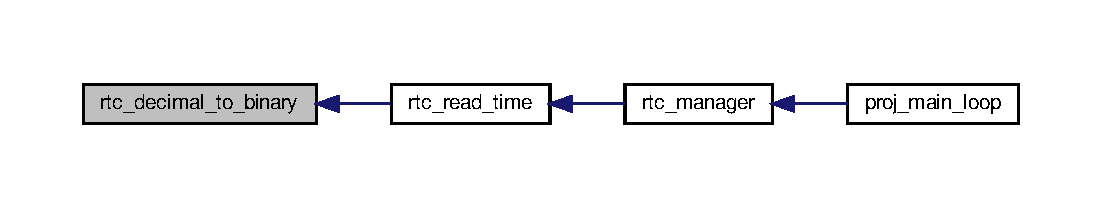
\includegraphics[width=350pt]{group__rtc_ga862729c9ed50edc422841b6b8bc5aa43_icgraph}
\end{center}
\end{figure}
\mbox{\Hypertarget{group__rtc_ga0f8758bf0df6766696104c3be6c0c6ea}\label{group__rtc_ga0f8758bf0df6766696104c3be6c0c6ea}} 
\index{Rtc@{Rtc}!rtc\+\_\+disable\+\_\+int@{rtc\+\_\+disable\+\_\+int}}
\index{rtc\+\_\+disable\+\_\+int@{rtc\+\_\+disable\+\_\+int}!Rtc@{Rtc}}
\subsubsection{\texorpdfstring{rtc\+\_\+disable\+\_\+int()}{rtc\_disable\_int()}}
{\footnotesize\ttfamily void rtc\+\_\+disable\+\_\+int (\begin{DoxyParamCaption}{ }\end{DoxyParamCaption})}



Function that disables R\+TC interruptions. 

\begin{DoxyReturn}{Returns}
Return 0 upon success 
\end{DoxyReturn}
Here is the call graph for this function\+:
\nopagebreak
\begin{figure}[H]
\begin{center}
\leavevmode
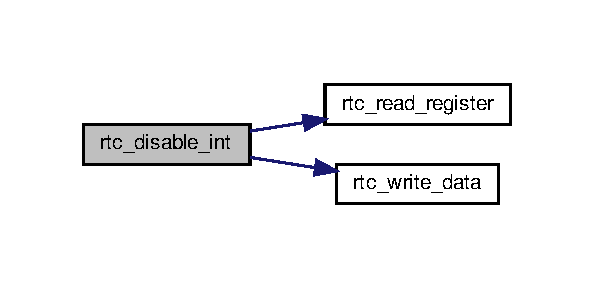
\includegraphics[width=285pt]{group__rtc_ga0f8758bf0df6766696104c3be6c0c6ea_cgraph}
\end{center}
\end{figure}
Here is the caller graph for this function\+:\nopagebreak
\begin{figure}[H]
\begin{center}
\leavevmode
\includegraphics[width=278pt]{group__rtc_ga0f8758bf0df6766696104c3be6c0c6ea_icgraph}
\end{center}
\end{figure}
\mbox{\Hypertarget{group__rtc_ga8d098a183fdb5fc38da0335041c4d3db}\label{group__rtc_ga8d098a183fdb5fc38da0335041c4d3db}} 
\index{Rtc@{Rtc}!rtc\+\_\+enable\+\_\+int@{rtc\+\_\+enable\+\_\+int}}
\index{rtc\+\_\+enable\+\_\+int@{rtc\+\_\+enable\+\_\+int}!Rtc@{Rtc}}
\subsubsection{\texorpdfstring{rtc\+\_\+enable\+\_\+int()}{rtc\_enable\_int()}}
{\footnotesize\ttfamily void rtc\+\_\+enable\+\_\+int (\begin{DoxyParamCaption}{ }\end{DoxyParamCaption})}



Function that enables R\+TC interruptions. 

\begin{DoxyReturn}{Returns}
Return 0 upon success 
\end{DoxyReturn}
Here is the call graph for this function\+:
\nopagebreak
\begin{figure}[H]
\begin{center}
\leavevmode
\includegraphics[width=282pt]{group__rtc_ga8d098a183fdb5fc38da0335041c4d3db_cgraph}
\end{center}
\end{figure}
Here is the caller graph for this function\+:\nopagebreak
\begin{figure}[H]
\begin{center}
\leavevmode
\includegraphics[width=275pt]{group__rtc_ga8d098a183fdb5fc38da0335041c4d3db_icgraph}
\end{center}
\end{figure}
\mbox{\Hypertarget{group__rtc_ga72153103ac037b1a162a9099f001b83c}\label{group__rtc_ga72153103ac037b1a162a9099f001b83c}} 
\index{Rtc@{Rtc}!rtc\+\_\+read\+\_\+register@{rtc\+\_\+read\+\_\+register}}
\index{rtc\+\_\+read\+\_\+register@{rtc\+\_\+read\+\_\+register}!Rtc@{Rtc}}
\subsubsection{\texorpdfstring{rtc\+\_\+read\+\_\+register()}{rtc\_read\_register()}}
{\footnotesize\ttfamily uint8\+\_\+t rtc\+\_\+read\+\_\+register (\begin{DoxyParamCaption}\item[{uint32\+\_\+t}]{port }\end{DoxyParamCaption})}



Function that reads from the register and reads on the returned variable. 


\begin{DoxyParams}{Parameters}
{\em port} & register wich you want to read from\\
\hline
\end{DoxyParams}
\begin{DoxyReturn}{Returns}
data from the register 
\end{DoxyReturn}
Here is the caller graph for this function\+:
\nopagebreak
\begin{figure}[H]
\begin{center}
\leavevmode
\includegraphics[width=350pt]{group__rtc_ga72153103ac037b1a162a9099f001b83c_icgraph}
\end{center}
\end{figure}
\mbox{\Hypertarget{group__rtc_ga94747f0e2c4ea5ae327017d78a25de30}\label{group__rtc_ga94747f0e2c4ea5ae327017d78a25de30}} 
\index{Rtc@{Rtc}!rtc\+\_\+read\+\_\+time@{rtc\+\_\+read\+\_\+time}}
\index{rtc\+\_\+read\+\_\+time@{rtc\+\_\+read\+\_\+time}!Rtc@{Rtc}}
\subsubsection{\texorpdfstring{rtc\+\_\+read\+\_\+time()}{rtc\_read\_time()}}
{\footnotesize\ttfamily void rtc\+\_\+read\+\_\+time (\begin{DoxyParamCaption}\item[{\hyperlink{structrtc__time}{rtc\+\_\+time} $\ast$}]{time }\end{DoxyParamCaption})}



Function that reads R\+TC\textquotesingle{}s hours, minutes and seconds and saves it on the R\+TC time struct. 


\begin{DoxyParams}{Parameters}
{\em time} & pointer to a variable of type struct \hyperlink{structrtc__time}{rtc\+\_\+time} \\
\hline
\end{DoxyParams}
Here is the call graph for this function\+:
\nopagebreak
\begin{figure}[H]
\begin{center}
\leavevmode
\includegraphics[width=304pt]{group__rtc_ga94747f0e2c4ea5ae327017d78a25de30_cgraph}
\end{center}
\end{figure}
Here is the caller graph for this function\+:
\nopagebreak
\begin{figure}[H]
\begin{center}
\leavevmode
\includegraphics[width=350pt]{group__rtc_ga94747f0e2c4ea5ae327017d78a25de30_icgraph}
\end{center}
\end{figure}
\mbox{\Hypertarget{group__rtc_gabd8de825e876e8ef94c64ac616f68a11}\label{group__rtc_gabd8de825e876e8ef94c64ac616f68a11}} 
\index{Rtc@{Rtc}!rtc\+\_\+subscribe\+\_\+int@{rtc\+\_\+subscribe\+\_\+int}}
\index{rtc\+\_\+subscribe\+\_\+int@{rtc\+\_\+subscribe\+\_\+int}!Rtc@{Rtc}}
\subsubsection{\texorpdfstring{rtc\+\_\+subscribe\+\_\+int()}{rtc\_subscribe\_int()}}
{\footnotesize\ttfamily int rtc\+\_\+subscribe\+\_\+int (\begin{DoxyParamCaption}{ }\end{DoxyParamCaption})}



Function that subscribes R\+TC interruptions. 

\begin{DoxyReturn}{Returns}
Return 0 upon success 
\end{DoxyReturn}
Here is the caller graph for this function\+:\nopagebreak
\begin{figure}[H]
\begin{center}
\leavevmode
\includegraphics[width=289pt]{group__rtc_gabd8de825e876e8ef94c64ac616f68a11_icgraph}
\end{center}
\end{figure}
\mbox{\Hypertarget{group__rtc_gab8f17bf5280c908c8b199a90fefcc758}\label{group__rtc_gab8f17bf5280c908c8b199a90fefcc758}} 
\index{Rtc@{Rtc}!rtc\+\_\+unsubscribe\+\_\+int@{rtc\+\_\+unsubscribe\+\_\+int}}
\index{rtc\+\_\+unsubscribe\+\_\+int@{rtc\+\_\+unsubscribe\+\_\+int}!Rtc@{Rtc}}
\subsubsection{\texorpdfstring{rtc\+\_\+unsubscribe\+\_\+int()}{rtc\_unsubscribe\_int()}}
{\footnotesize\ttfamily int rtc\+\_\+unsubscribe\+\_\+int (\begin{DoxyParamCaption}{ }\end{DoxyParamCaption})}



Function that unsubscribes R\+TC interruptions. 

\begin{DoxyReturn}{Returns}
Return 0 upon success 
\end{DoxyReturn}
Here is the caller graph for this function\+:\nopagebreak
\begin{figure}[H]
\begin{center}
\leavevmode
\includegraphics[width=299pt]{group__rtc_gab8f17bf5280c908c8b199a90fefcc758_icgraph}
\end{center}
\end{figure}
\mbox{\Hypertarget{group__rtc_gade198e3189c6f8195cde4e404671f980}\label{group__rtc_gade198e3189c6f8195cde4e404671f980}} 
\index{Rtc@{Rtc}!rtc\+\_\+write\+\_\+data@{rtc\+\_\+write\+\_\+data}}
\index{rtc\+\_\+write\+\_\+data@{rtc\+\_\+write\+\_\+data}!Rtc@{Rtc}}
\subsubsection{\texorpdfstring{rtc\+\_\+write\+\_\+data()}{rtc\_write\_data()}}
{\footnotesize\ttfamily void rtc\+\_\+write\+\_\+data (\begin{DoxyParamCaption}\item[{uint32\+\_\+t}]{port,  }\item[{uint32\+\_\+t}]{data }\end{DoxyParamCaption})}



Function that writes data to a register. 


\begin{DoxyParams}{Parameters}
{\em port} & register in which you want to write \\
\hline
{\em data} & value that is gonna be written to the register \\
\hline
\end{DoxyParams}
Here is the caller graph for this function\+:
\nopagebreak
\begin{figure}[H]
\begin{center}
\leavevmode
\includegraphics[width=350pt]{group__rtc_gade198e3189c6f8195cde4e404671f980_icgraph}
\end{center}
\end{figure}

\hypertarget{group__timer}{}\section{timer}
\label{group__timer}\index{timer@{timer}}
\subsection*{Data Structures}
\begin{DoxyCompactItemize}
\item 
union \hyperlink{uniontimer__status__field__val}{timer\+\_\+status\+\_\+field\+\_\+val}
\begin{DoxyCompactList}\small\item\em Union for storing values of timer status fields, including the full status byte. \end{DoxyCompactList}\end{DoxyCompactItemize}
\subsection*{Enumerations}
\begin{DoxyCompactItemize}
\item 
enum \hyperlink{group__timer_ga5cc20f14fd50625eea9b20f58fbe2a55}{timer\+\_\+init} \{ \hyperlink{group__timer_gga5cc20f14fd50625eea9b20f58fbe2a55a829d958875d8e92068f1b07f858721a4}{I\+N\+V\+A\+L\+\_\+val}, 
\hyperlink{group__timer_gga5cc20f14fd50625eea9b20f58fbe2a55a9a2e8b22f6d5ee33cc37829164a55955}{L\+S\+B\+\_\+only}, 
\hyperlink{group__timer_gga5cc20f14fd50625eea9b20f58fbe2a55ae46d93c3576b5f78ae1aeb4ee4fc4938}{M\+S\+B\+\_\+only}, 
\hyperlink{group__timer_gga5cc20f14fd50625eea9b20f58fbe2a55a7d392c02b4f52d93c10e4c646f8cedc7}{M\+S\+B\+\_\+after\+\_\+\+L\+SB}
 \}\begin{DoxyCompactList}\small\item\em Enumerated type for specifying the timer value initialization. \end{DoxyCompactList}
\item 
enum \hyperlink{group__timer_gada782f3116a896caaa602b70c0c6d8b7}{timer\+\_\+status\+\_\+field} \{ \hyperlink{group__timer_ggada782f3116a896caaa602b70c0c6d8b7a92376d84969da91547254fc7461f0da2}{tsf\+\_\+all}, 
\hyperlink{group__timer_ggada782f3116a896caaa602b70c0c6d8b7aa89f72faf31fa0e4db8cab25364a4583}{tsf\+\_\+initial}, 
\hyperlink{group__timer_ggada782f3116a896caaa602b70c0c6d8b7aa84c2f6462a2deb90fda229c89453dfa}{tsf\+\_\+mode}, 
\hyperlink{group__timer_ggada782f3116a896caaa602b70c0c6d8b7af4b69eace6b1cc952de198acee4c5e32}{tsf\+\_\+base}
 \}\begin{DoxyCompactList}\small\item\em Enumerated type for identifying the timer status fields. \end{DoxyCompactList}
\end{DoxyCompactItemize}
\subsection*{Functions}
\begin{DoxyCompactItemize}
\item 
int() \hyperlink{group__timer_gaf2c04fa8e97ffa748fd3f612886a92a7}{timer\+\_\+set\+\_\+frequency} (uint8\+\_\+t timer, uint32\+\_\+t freq)
\begin{DoxyCompactList}\small\item\em Changes the operating frequency of a timer. \end{DoxyCompactList}\item 
int() \hyperlink{group__timer_gac57a7e1140a7e00ad95ac5488d2a671b}{timer\+\_\+subscribe\+\_\+int} (uint8\+\_\+t $\ast$bit\+\_\+no)
\begin{DoxyCompactList}\small\item\em Subscribes and enables Timer 0 interrupts. \end{DoxyCompactList}\item 
int() \hyperlink{group__timer_gafabd21de449be154dd65d5fdb2d8045d}{timer\+\_\+unsubscribe\+\_\+int} ()
\begin{DoxyCompactList}\small\item\em Unsubscribes Timer 0 interrupts. \end{DoxyCompactList}\item 
void() \hyperlink{group__timer_ga91a2072306c68353712a6b771287dc2c}{timer\+\_\+int\+\_\+handler} ()
\begin{DoxyCompactList}\small\item\em Timer 0 interrupt handler. \end{DoxyCompactList}\item 
int() \hyperlink{group__timer_ga703c60b40c8c49607d6ecb6fef82d27a}{timer\+\_\+get\+\_\+conf} (uint8\+\_\+t timer, uint8\+\_\+t $\ast$st)
\begin{DoxyCompactList}\small\item\em Reads the input timer configuration (status) via read-\/back command. \end{DoxyCompactList}\item 
int() \hyperlink{group__timer_ga140d8f092c0913cabdca949c4a1cc650}{timer\+\_\+display\+\_\+conf} (uint8\+\_\+t timer, uint8\+\_\+t st, enum \hyperlink{group__timer_gada782f3116a896caaa602b70c0c6d8b7}{timer\+\_\+status\+\_\+field} field)
\begin{DoxyCompactList}\small\item\em Shows timer configuration. \end{DoxyCompactList}\item 
int() \hyperlink{group__timer_gad3902e029b27c80982873394c0290496}{timer\+\_\+print\+\_\+config} (uint8\+\_\+t timer, enum \hyperlink{group__timer_gada782f3116a896caaa602b70c0c6d8b7}{timer\+\_\+status\+\_\+field} field, union \hyperlink{uniontimer__status__field__val}{timer\+\_\+status\+\_\+field\+\_\+val} val)
\begin{DoxyCompactList}\small\item\em Prints a timer config field value. \end{DoxyCompactList}\item 
uint32\+\_\+t() \hyperlink{group__timer_ga43b221cba0c39b32f89688dcfee5aefa}{timer\+\_\+print\+\_\+elapsed\+\_\+time} ()
\begin{DoxyCompactList}\small\item\em Increments elapsed time count. \end{DoxyCompactList}\end{DoxyCompactItemize}
\subsection*{Variables}
\begin{DoxyCompactItemize}
\item 
uint8\+\_\+t \hyperlink{group__timer_ga96f44d20f1dbf1c8785a7bc99a46164c}{byte}
\item 
enum \hyperlink{group__timer_ga5cc20f14fd50625eea9b20f58fbe2a55}{timer\+\_\+init} \hyperlink{group__timer_gad414fb8742e435f9bda1f199a6200645}{in\+\_\+mode}
\item 
uint8\+\_\+t \hyperlink{group__timer_gabd6e94a182fc2daff67dfb46f732644a}{count\+\_\+mode}
\item 
bool \hyperlink{group__timer_gaa2444cde256beeae6fb06bb7a5ebd0c9}{bcd}
\end{DoxyCompactItemize}


\subsection{Detailed Description}
Functions for using the i8254 timers 

\subsection{Enumeration Type Documentation}
\mbox{\Hypertarget{group__timer_ga5cc20f14fd50625eea9b20f58fbe2a55}\label{group__timer_ga5cc20f14fd50625eea9b20f58fbe2a55}} 
\index{timer@{timer}!timer\+\_\+init@{timer\+\_\+init}}
\index{timer\+\_\+init@{timer\+\_\+init}!timer@{timer}}
\subsubsection{\texorpdfstring{timer\+\_\+init}{timer\_init}}
{\footnotesize\ttfamily enum \hyperlink{group__timer_ga5cc20f14fd50625eea9b20f58fbe2a55}{timer\+\_\+init}}



Enumerated type for specifying the timer value initialization. 

\begin{DoxyEnumFields}{Enumerator}
\raisebox{\heightof{T}}[0pt][0pt]{\index{I\+N\+V\+A\+L\+\_\+val@{I\+N\+V\+A\+L\+\_\+val}!timer@{timer}}\index{timer@{timer}!I\+N\+V\+A\+L\+\_\+val@{I\+N\+V\+A\+L\+\_\+val}}}\mbox{\Hypertarget{group__timer_gga5cc20f14fd50625eea9b20f58fbe2a55a829d958875d8e92068f1b07f858721a4}\label{group__timer_gga5cc20f14fd50625eea9b20f58fbe2a55a829d958875d8e92068f1b07f858721a4}} 
I\+N\+V\+A\+L\+\_\+val&Invalid initialization mode \\
\hline

\raisebox{\heightof{T}}[0pt][0pt]{\index{L\+S\+B\+\_\+only@{L\+S\+B\+\_\+only}!timer@{timer}}\index{timer@{timer}!L\+S\+B\+\_\+only@{L\+S\+B\+\_\+only}}}\mbox{\Hypertarget{group__timer_gga5cc20f14fd50625eea9b20f58fbe2a55a9a2e8b22f6d5ee33cc37829164a55955}\label{group__timer_gga5cc20f14fd50625eea9b20f58fbe2a55a9a2e8b22f6d5ee33cc37829164a55955}} 
L\+S\+B\+\_\+only&Initialization only of the L\+SB \\
\hline

\raisebox{\heightof{T}}[0pt][0pt]{\index{M\+S\+B\+\_\+only@{M\+S\+B\+\_\+only}!timer@{timer}}\index{timer@{timer}!M\+S\+B\+\_\+only@{M\+S\+B\+\_\+only}}}\mbox{\Hypertarget{group__timer_gga5cc20f14fd50625eea9b20f58fbe2a55ae46d93c3576b5f78ae1aeb4ee4fc4938}\label{group__timer_gga5cc20f14fd50625eea9b20f58fbe2a55ae46d93c3576b5f78ae1aeb4ee4fc4938}} 
M\+S\+B\+\_\+only&Initialization only of the M\+SB \\
\hline

\raisebox{\heightof{T}}[0pt][0pt]{\index{M\+S\+B\+\_\+after\+\_\+\+L\+SB@{M\+S\+B\+\_\+after\+\_\+\+L\+SB}!timer@{timer}}\index{timer@{timer}!M\+S\+B\+\_\+after\+\_\+\+L\+SB@{M\+S\+B\+\_\+after\+\_\+\+L\+SB}}}\mbox{\Hypertarget{group__timer_gga5cc20f14fd50625eea9b20f58fbe2a55a7d392c02b4f52d93c10e4c646f8cedc7}\label{group__timer_gga5cc20f14fd50625eea9b20f58fbe2a55a7d392c02b4f52d93c10e4c646f8cedc7}} 
M\+S\+B\+\_\+after\+\_\+\+L\+SB&Initialization of L\+SB and M\+SB, in this order \\
\hline

\end{DoxyEnumFields}
\mbox{\Hypertarget{group__timer_gada782f3116a896caaa602b70c0c6d8b7}\label{group__timer_gada782f3116a896caaa602b70c0c6d8b7}} 
\index{timer@{timer}!timer\+\_\+status\+\_\+field@{timer\+\_\+status\+\_\+field}}
\index{timer\+\_\+status\+\_\+field@{timer\+\_\+status\+\_\+field}!timer@{timer}}
\subsubsection{\texorpdfstring{timer\+\_\+status\+\_\+field}{timer\_status\_field}}
{\footnotesize\ttfamily enum \hyperlink{group__timer_gada782f3116a896caaa602b70c0c6d8b7}{timer\+\_\+status\+\_\+field}}



Enumerated type for identifying the timer status fields. 

\begin{DoxyEnumFields}{Enumerator}
\raisebox{\heightof{T}}[0pt][0pt]{\index{tsf\+\_\+all@{tsf\+\_\+all}!timer@{timer}}\index{timer@{timer}!tsf\+\_\+all@{tsf\+\_\+all}}}\mbox{\Hypertarget{group__timer_ggada782f3116a896caaa602b70c0c6d8b7a92376d84969da91547254fc7461f0da2}\label{group__timer_ggada782f3116a896caaa602b70c0c6d8b7a92376d84969da91547254fc7461f0da2}} 
tsf\+\_\+all&configuration/status \\
\hline

\raisebox{\heightof{T}}[0pt][0pt]{\index{tsf\+\_\+initial@{tsf\+\_\+initial}!timer@{timer}}\index{timer@{timer}!tsf\+\_\+initial@{tsf\+\_\+initial}}}\mbox{\Hypertarget{group__timer_ggada782f3116a896caaa602b70c0c6d8b7aa89f72faf31fa0e4db8cab25364a4583}\label{group__timer_ggada782f3116a896caaa602b70c0c6d8b7aa89f72faf31fa0e4db8cab25364a4583}} 
tsf\+\_\+initial&timer initialization mode \\
\hline

\raisebox{\heightof{T}}[0pt][0pt]{\index{tsf\+\_\+mode@{tsf\+\_\+mode}!timer@{timer}}\index{timer@{timer}!tsf\+\_\+mode@{tsf\+\_\+mode}}}\mbox{\Hypertarget{group__timer_ggada782f3116a896caaa602b70c0c6d8b7aa84c2f6462a2deb90fda229c89453dfa}\label{group__timer_ggada782f3116a896caaa602b70c0c6d8b7aa84c2f6462a2deb90fda229c89453dfa}} 
tsf\+\_\+mode&timer counting mode \\
\hline

\raisebox{\heightof{T}}[0pt][0pt]{\index{tsf\+\_\+base@{tsf\+\_\+base}!timer@{timer}}\index{timer@{timer}!tsf\+\_\+base@{tsf\+\_\+base}}}\mbox{\Hypertarget{group__timer_ggada782f3116a896caaa602b70c0c6d8b7af4b69eace6b1cc952de198acee4c5e32}\label{group__timer_ggada782f3116a896caaa602b70c0c6d8b7af4b69eace6b1cc952de198acee4c5e32}} 
tsf\+\_\+base&timer counting base \\
\hline

\end{DoxyEnumFields}


\subsection{Function Documentation}
\mbox{\Hypertarget{group__timer_ga140d8f092c0913cabdca949c4a1cc650}\label{group__timer_ga140d8f092c0913cabdca949c4a1cc650}} 
\index{timer@{timer}!timer\+\_\+display\+\_\+conf@{timer\+\_\+display\+\_\+conf}}
\index{timer\+\_\+display\+\_\+conf@{timer\+\_\+display\+\_\+conf}!timer@{timer}}
\subsubsection{\texorpdfstring{timer\+\_\+display\+\_\+conf()}{timer\_display\_conf()}}
{\footnotesize\ttfamily int() timer\+\_\+display\+\_\+conf (\begin{DoxyParamCaption}\item[{uint8\+\_\+t}]{timer,  }\item[{uint8\+\_\+t}]{st,  }\item[{enum \hyperlink{group__timer_gada782f3116a896caaa602b70c0c6d8b7}{timer\+\_\+status\+\_\+field}}]{field }\end{DoxyParamCaption})}



Shows timer configuration. 

Displays, in a human friendly way, the specified field of a timer status, which was read via the read-\/back command


\begin{DoxyParams}{Parameters}
{\em timer} & timer whose configuration should be displayed (Ranges from 0 to 2) \\
\hline
{\em st} & status read via the read-\/back command \\
\hline
{\em field} & status field to display in human friendly way \\
\hline
\end{DoxyParams}
\begin{DoxyReturn}{Returns}
Return 0 upon success and non-\/zero otherwise 
\end{DoxyReturn}
Here is the call graph for this function\+:\nopagebreak
\begin{figure}[H]
\begin{center}
\leavevmode
\includegraphics[width=308pt]{group__timer_ga140d8f092c0913cabdca949c4a1cc650_cgraph}
\end{center}
\end{figure}
\mbox{\Hypertarget{group__timer_ga703c60b40c8c49607d6ecb6fef82d27a}\label{group__timer_ga703c60b40c8c49607d6ecb6fef82d27a}} 
\index{timer@{timer}!timer\+\_\+get\+\_\+conf@{timer\+\_\+get\+\_\+conf}}
\index{timer\+\_\+get\+\_\+conf@{timer\+\_\+get\+\_\+conf}!timer@{timer}}
\subsubsection{\texorpdfstring{timer\+\_\+get\+\_\+conf()}{timer\_get\_conf()}}
{\footnotesize\ttfamily int() timer\+\_\+get\+\_\+conf (\begin{DoxyParamCaption}\item[{uint8\+\_\+t}]{timer,  }\item[{uint8\+\_\+t $\ast$}]{st }\end{DoxyParamCaption})}



Reads the input timer configuration (status) via read-\/back command. 


\begin{DoxyParams}{Parameters}
{\em timer} & Timer whose configuration to read (Ranges from 0 to 2) \\
\hline
{\em st} & Address of memory position to be filled with the timer config \\
\hline
\end{DoxyParams}
\begin{DoxyReturn}{Returns}
Return 0 upon success and non-\/zero otherwise 
\end{DoxyReturn}
Here is the caller graph for this function\+:\nopagebreak
\begin{figure}[H]
\begin{center}
\leavevmode
\includegraphics[width=302pt]{group__timer_ga703c60b40c8c49607d6ecb6fef82d27a_icgraph}
\end{center}
\end{figure}
\mbox{\Hypertarget{group__timer_ga91a2072306c68353712a6b771287dc2c}\label{group__timer_ga91a2072306c68353712a6b771287dc2c}} 
\index{timer@{timer}!timer\+\_\+int\+\_\+handler@{timer\+\_\+int\+\_\+handler}}
\index{timer\+\_\+int\+\_\+handler@{timer\+\_\+int\+\_\+handler}!timer@{timer}}
\subsubsection{\texorpdfstring{timer\+\_\+int\+\_\+handler()}{timer\_int\_handler()}}
{\footnotesize\ttfamily void() timer\+\_\+int\+\_\+handler (\begin{DoxyParamCaption}{ }\end{DoxyParamCaption})}



Timer 0 interrupt handler. 

Increments counter Here is the caller graph for this function\+:
\nopagebreak
\begin{figure}[H]
\begin{center}
\leavevmode
\includegraphics[width=350pt]{group__timer_ga91a2072306c68353712a6b771287dc2c_icgraph}
\end{center}
\end{figure}
\mbox{\Hypertarget{group__timer_gad3902e029b27c80982873394c0290496}\label{group__timer_gad3902e029b27c80982873394c0290496}} 
\index{timer@{timer}!timer\+\_\+print\+\_\+config@{timer\+\_\+print\+\_\+config}}
\index{timer\+\_\+print\+\_\+config@{timer\+\_\+print\+\_\+config}!timer@{timer}}
\subsubsection{\texorpdfstring{timer\+\_\+print\+\_\+config()}{timer\_print\_config()}}
{\footnotesize\ttfamily int() timer\+\_\+print\+\_\+config (\begin{DoxyParamCaption}\item[{uint8\+\_\+t}]{timer,  }\item[{enum \hyperlink{group__timer_gada782f3116a896caaa602b70c0c6d8b7}{timer\+\_\+status\+\_\+field}}]{field,  }\item[{union \hyperlink{uniontimer__status__field__val}{timer\+\_\+status\+\_\+field\+\_\+val}}]{val }\end{DoxyParamCaption})}



Prints a timer config field value. 

\begin{DoxyReturn}{Returns}
Returns 0 upon success and non-\/zero otherwise 
\end{DoxyReturn}
Here is the caller graph for this function\+:
\nopagebreak
\begin{figure}[H]
\begin{center}
\leavevmode
\includegraphics[width=308pt]{group__timer_gad3902e029b27c80982873394c0290496_icgraph}
\end{center}
\end{figure}
\mbox{\Hypertarget{group__timer_ga43b221cba0c39b32f89688dcfee5aefa}\label{group__timer_ga43b221cba0c39b32f89688dcfee5aefa}} 
\index{timer@{timer}!timer\+\_\+print\+\_\+elapsed\+\_\+time@{timer\+\_\+print\+\_\+elapsed\+\_\+time}}
\index{timer\+\_\+print\+\_\+elapsed\+\_\+time@{timer\+\_\+print\+\_\+elapsed\+\_\+time}!timer@{timer}}
\subsubsection{\texorpdfstring{timer\+\_\+print\+\_\+elapsed\+\_\+time()}{timer\_print\_elapsed\_time()}}
{\footnotesize\ttfamily uint32\+\_\+t() timer\+\_\+print\+\_\+elapsed\+\_\+time (\begin{DoxyParamCaption}{ }\end{DoxyParamCaption})}



Increments elapsed time count. 

\begin{DoxyReturn}{Returns}
Returns the current time count 
\end{DoxyReturn}
\mbox{\Hypertarget{group__timer_gaf2c04fa8e97ffa748fd3f612886a92a7}\label{group__timer_gaf2c04fa8e97ffa748fd3f612886a92a7}} 
\index{timer@{timer}!timer\+\_\+set\+\_\+frequency@{timer\+\_\+set\+\_\+frequency}}
\index{timer\+\_\+set\+\_\+frequency@{timer\+\_\+set\+\_\+frequency}!timer@{timer}}
\subsubsection{\texorpdfstring{timer\+\_\+set\+\_\+frequency()}{timer\_set\_frequency()}}
{\footnotesize\ttfamily int() timer\+\_\+set\+\_\+frequency (\begin{DoxyParamCaption}\item[{uint8\+\_\+t}]{timer,  }\item[{uint32\+\_\+t}]{freq }\end{DoxyParamCaption})}



Changes the operating frequency of a timer. 

Must use the read-\/back command so that it does not change the 4 L\+S\+Bs (mode and B\+C\+D/binary) of the timer\textquotesingle{}s control word.


\begin{DoxyParams}{Parameters}
{\em timer} & Timer to configure. (Ranges from 0 to 2) \\
\hline
{\em freq} & Timer operating frequency \\
\hline
\end{DoxyParams}
\begin{DoxyReturn}{Returns}
Return 0 upon success and non-\/zero otherwise 
\end{DoxyReturn}
Here is the call graph for this function\+:
\nopagebreak
\begin{figure}[H]
\begin{center}
\leavevmode
\includegraphics[width=302pt]{group__timer_gaf2c04fa8e97ffa748fd3f612886a92a7_cgraph}
\end{center}
\end{figure}
\mbox{\Hypertarget{group__timer_gac57a7e1140a7e00ad95ac5488d2a671b}\label{group__timer_gac57a7e1140a7e00ad95ac5488d2a671b}} 
\index{timer@{timer}!timer\+\_\+subscribe\+\_\+int@{timer\+\_\+subscribe\+\_\+int}}
\index{timer\+\_\+subscribe\+\_\+int@{timer\+\_\+subscribe\+\_\+int}!timer@{timer}}
\subsubsection{\texorpdfstring{timer\+\_\+subscribe\+\_\+int()}{timer\_subscribe\_int()}}
{\footnotesize\ttfamily int() timer\+\_\+subscribe\+\_\+int (\begin{DoxyParamCaption}\item[{uint8\+\_\+t $\ast$}]{bit\+\_\+no }\end{DoxyParamCaption})}



Subscribes and enables Timer 0 interrupts. 


\begin{DoxyParams}{Parameters}
{\em bit\+\_\+no} & address of memory to be initialized with the bit number to be set in the mask returned upon an interrupt \\
\hline
\end{DoxyParams}
\begin{DoxyReturn}{Returns}
Return 0 upon success and non-\/zero otherwise 
\end{DoxyReturn}
Here is the caller graph for this function\+:\nopagebreak
\begin{figure}[H]
\begin{center}
\leavevmode
\includegraphics[width=299pt]{group__timer_gac57a7e1140a7e00ad95ac5488d2a671b_icgraph}
\end{center}
\end{figure}
\mbox{\Hypertarget{group__timer_gafabd21de449be154dd65d5fdb2d8045d}\label{group__timer_gafabd21de449be154dd65d5fdb2d8045d}} 
\index{timer@{timer}!timer\+\_\+unsubscribe\+\_\+int@{timer\+\_\+unsubscribe\+\_\+int}}
\index{timer\+\_\+unsubscribe\+\_\+int@{timer\+\_\+unsubscribe\+\_\+int}!timer@{timer}}
\subsubsection{\texorpdfstring{timer\+\_\+unsubscribe\+\_\+int()}{timer\_unsubscribe\_int()}}
{\footnotesize\ttfamily int() timer\+\_\+unsubscribe\+\_\+int (\begin{DoxyParamCaption}{ }\end{DoxyParamCaption})}



Unsubscribes Timer 0 interrupts. 

\begin{DoxyReturn}{Returns}
Return 0 upon success and non-\/zero otherwise 
\end{DoxyReturn}
Here is the caller graph for this function\+:\nopagebreak
\begin{figure}[H]
\begin{center}
\leavevmode
\includegraphics[width=310pt]{group__timer_gafabd21de449be154dd65d5fdb2d8045d_icgraph}
\end{center}
\end{figure}


\subsection{Variable Documentation}
\mbox{\Hypertarget{group__timer_gaa2444cde256beeae6fb06bb7a5ebd0c9}\label{group__timer_gaa2444cde256beeae6fb06bb7a5ebd0c9}} 
\index{timer@{timer}!bcd@{bcd}}
\index{bcd@{bcd}!timer@{timer}}
\subsubsection{\texorpdfstring{bcd}{bcd}}
{\footnotesize\ttfamily bool bcd}

counting base, true if B\+CD \mbox{\Hypertarget{group__timer_ga96f44d20f1dbf1c8785a7bc99a46164c}\label{group__timer_ga96f44d20f1dbf1c8785a7bc99a46164c}} 
\index{timer@{timer}!byte@{byte}}
\index{byte@{byte}!timer@{timer}}
\subsubsection{\texorpdfstring{byte}{byte}}
{\footnotesize\ttfamily uint8\+\_\+t byte}

status \mbox{\Hypertarget{group__timer_gabd6e94a182fc2daff67dfb46f732644a}\label{group__timer_gabd6e94a182fc2daff67dfb46f732644a}} 
\index{timer@{timer}!count\+\_\+mode@{count\+\_\+mode}}
\index{count\+\_\+mode@{count\+\_\+mode}!timer@{timer}}
\subsubsection{\texorpdfstring{count\+\_\+mode}{count\_mode}}
{\footnotesize\ttfamily uint8\+\_\+t count\+\_\+mode}

counting mode\+: 0, 1,.., 5 \mbox{\Hypertarget{group__timer_gad414fb8742e435f9bda1f199a6200645}\label{group__timer_gad414fb8742e435f9bda1f199a6200645}} 
\index{timer@{timer}!in\+\_\+mode@{in\+\_\+mode}}
\index{in\+\_\+mode@{in\+\_\+mode}!timer@{timer}}
\subsubsection{\texorpdfstring{in\+\_\+mode}{in\_mode}}
{\footnotesize\ttfamily enum \hyperlink{group__timer_ga5cc20f14fd50625eea9b20f58fbe2a55}{timer\+\_\+init} in\+\_\+mode}

initialization mode 
\hypertarget{group__types}{}\section{Types}
\label{group__types}\index{Types@{Types}}
\subsection*{Enumerations}
\begin{DoxyCompactItemize}
\item 
enum \hyperlink{group__types_ga210774229705ea136db591a108c52d39}{sleep\+\_\+bar} \{ \hyperlink{group__types_gga210774229705ea136db591a108c52d39a34b8ae25d2c59204b94c7f59f8807ddc}{S\+L\+E\+E\+P\+\_\+4}, 
\hyperlink{group__types_gga210774229705ea136db591a108c52d39a373243d2c5eab6e7ccd90cd7b00ac6a0}{S\+L\+E\+E\+P\+\_\+3}, 
\hyperlink{group__types_gga210774229705ea136db591a108c52d39adb15ec35d217dd149a609869ad8965b0}{S\+L\+E\+E\+P\+\_\+2}, 
\hyperlink{group__types_gga210774229705ea136db591a108c52d39a99607e587be600c9c78736442f98e0c2}{S\+L\+E\+E\+P\+\_\+1}
 \}\begin{DoxyCompactList}\small\item\em Different modes of the sleep bar. \end{DoxyCompactList}
\item 
enum \hyperlink{group__types_ga68b33015e0d4635ee8ddb795eca9d963}{food\+\_\+bar} \{ \hyperlink{group__types_gga68b33015e0d4635ee8ddb795eca9d963ae6087a2b6ba833555ae35b9de54b8e45}{F\+O\+O\+D\+\_\+4}, 
\hyperlink{group__types_gga68b33015e0d4635ee8ddb795eca9d963ac101e2bc1eec1f422377d7666426db82}{F\+O\+O\+D\+\_\+3}, 
\hyperlink{group__types_gga68b33015e0d4635ee8ddb795eca9d963a201d01c246ac3967468218ee0e0eed60}{F\+O\+O\+D\+\_\+2}, 
\hyperlink{group__types_gga68b33015e0d4635ee8ddb795eca9d963aa058aeefefb2b143937d5cc840b357f2}{F\+O\+O\+D\+\_\+1}
 \}\begin{DoxyCompactList}\small\item\em Different modes of the food bar. \end{DoxyCompactList}
\item 
enum \hyperlink{group__types_gaac3396b3def300539a13396b352b7fca}{play\+\_\+bar} \{ \hyperlink{group__types_ggaac3396b3def300539a13396b352b7fcaaa4dc96448892c4533363f7f439d56c7c}{P\+L\+A\+Y\+\_\+4}, 
\hyperlink{group__types_ggaac3396b3def300539a13396b352b7fcaad398f358fe0160f104878a392f770d73}{P\+L\+A\+Y\+\_\+3}, 
\hyperlink{group__types_ggaac3396b3def300539a13396b352b7fcaa4a6603bd358878efd0d21a7968674d42}{P\+L\+A\+Y\+\_\+2}, 
\hyperlink{group__types_ggaac3396b3def300539a13396b352b7fcaa8da632afe00bac8c0fcc2d5a3d648e81}{P\+L\+A\+Y\+\_\+1}
 \}\begin{DoxyCompactList}\small\item\em Different modes of the fun bar. \end{DoxyCompactList}
\item 
enum \hyperlink{group__types_gad48fe05a3e5df355707b5a3fd6cf9d8e}{counter\+\_\+bar} \{ \newline
\hyperlink{group__types_ggad48fe05a3e5df355707b5a3fd6cf9d8ea744b56171f60c413fa330544e4313a65}{C00}, 
\hyperlink{group__types_ggad48fe05a3e5df355707b5a3fd6cf9d8ea78b3960a210c67998150d1f30d666469}{C01}, 
\hyperlink{group__types_ggad48fe05a3e5df355707b5a3fd6cf9d8ea201d3417f9556041ede319423b96c6b1}{C02}, 
\hyperlink{group__types_ggad48fe05a3e5df355707b5a3fd6cf9d8ea5f559b16b4abb722563277805166d8dd}{C03}, 
\newline
\hyperlink{group__types_ggad48fe05a3e5df355707b5a3fd6cf9d8ea51e9c517f19141a27e3bfcfc76d4e560}{C04}, 
\hyperlink{group__types_ggad48fe05a3e5df355707b5a3fd6cf9d8ea0ee81703668ecff2f0ca223f338ebfc2}{C05}, 
\hyperlink{group__types_ggad48fe05a3e5df355707b5a3fd6cf9d8ea45f511625d2ddbe62359693360630480}{C06}, 
\hyperlink{group__types_ggad48fe05a3e5df355707b5a3fd6cf9d8eae9f285207e9062092af134b5c546483d}{C07}, 
\newline
\hyperlink{group__types_ggad48fe05a3e5df355707b5a3fd6cf9d8eadb9c94eacc2d21898edbdc18102b8291}{C08}, 
\hyperlink{group__types_ggad48fe05a3e5df355707b5a3fd6cf9d8eaae5e18e46b7bb2982647b3fa46cb9810}{C09}, 
\hyperlink{group__types_ggad48fe05a3e5df355707b5a3fd6cf9d8ea561c7886c8c962cd1cfbe5224aba0433}{C10}, 
\hyperlink{group__types_ggad48fe05a3e5df355707b5a3fd6cf9d8ea248f378009f5666577feebae32471dc9}{C11}, 
\newline
\hyperlink{group__types_ggad48fe05a3e5df355707b5a3fd6cf9d8eadaa660cfb7228c48662e07375e4fa1d4}{C12}, 
\hyperlink{group__types_ggad48fe05a3e5df355707b5a3fd6cf9d8ea5656218db219787b8c3aa5cb7b842c9a}{C13}, 
\hyperlink{group__types_ggad48fe05a3e5df355707b5a3fd6cf9d8ea58614e79da8882248ff0c77e4b5c2fab}{C14}, 
\hyperlink{group__types_ggad48fe05a3e5df355707b5a3fd6cf9d8ea44e57b416f85a1658bb39d74638413ba}{C15}
 \}\begin{DoxyCompactList}\small\item\em Different values of the counter. \end{DoxyCompactList}
\item 
enum \hyperlink{group__types_ga7e8dce2e0fc3ad3b4e20b07886fa11d6}{cloud\+\_\+position} \{ \hyperlink{group__types_gga7e8dce2e0fc3ad3b4e20b07886fa11d6ab0ac36b187aa60c167ffcead3d5a03c0}{left}, 
\hyperlink{group__types_gga7e8dce2e0fc3ad3b4e20b07886fa11d6ac6c4bfa285e112c6854a2d820f854e3b}{center}, 
\hyperlink{group__types_gga7e8dce2e0fc3ad3b4e20b07886fa11d6af763d610923b0c4614e8ecd65212666a}{right}
 \}\begin{DoxyCompactList}\small\item\em Different positions of the cloud. \end{DoxyCompactList}
\item 
enum \hyperlink{group__types_gab5d0fdad1621cc17d1147dedd2e7a773}{score\+\_\+bar\+\_\+1} \{ \newline
\hyperlink{group__types_ggab5d0fdad1621cc17d1147dedd2e7a773a4859b519b5c8f30f648b008dc84aec4b}{S01}, 
\hyperlink{group__types_ggab5d0fdad1621cc17d1147dedd2e7a773a184077cf5dd86c87896e9d5d1f3b7ee0}{S02}, 
\hyperlink{group__types_ggab5d0fdad1621cc17d1147dedd2e7a773a86c78be85215eca7905bd2fd25830b27}{S03}, 
\hyperlink{group__types_ggab5d0fdad1621cc17d1147dedd2e7a773acc5d4a832b4d09833ef29f55a48aa199}{S04}, 
\newline
\hyperlink{group__types_ggab5d0fdad1621cc17d1147dedd2e7a773a71c3f05ae23db4a70e5274192b999213}{S05}, 
\hyperlink{group__types_ggab5d0fdad1621cc17d1147dedd2e7a773a246af4d015fb374806b4ff8b1c96626b}{S06}, 
\hyperlink{group__types_ggab5d0fdad1621cc17d1147dedd2e7a773a9015575afa20c4c87ce7df46008cf08f}{S07}, 
\hyperlink{group__types_ggab5d0fdad1621cc17d1147dedd2e7a773af4101f0b2006182144f1aed09f598246}{S08}, 
\newline
\hyperlink{group__types_ggab5d0fdad1621cc17d1147dedd2e7a773af59eda6225bd8cf7ead1eac101aba02e}{S09}, 
\hyperlink{group__types_ggab5d0fdad1621cc17d1147dedd2e7a773a7b217ba51ef5b37a307a790152efc0c6}{S00\+\_\+1}
 \}\begin{DoxyCompactList}\small\item\em Different values of the units of the score. \end{DoxyCompactList}
\item 
enum \hyperlink{group__types_gabd8d88ed6ba2aef17eb45496d20be732}{score\+\_\+bar\+\_\+2} \{ \newline
\hyperlink{group__types_ggabd8d88ed6ba2aef17eb45496d20be732a29356491726837ae48da1c049dbbf39b}{S10}, 
\hyperlink{group__types_ggabd8d88ed6ba2aef17eb45496d20be732a691ba8e46c2a3a3276c3e8f8e2c929d0}{S20}, 
\hyperlink{group__types_ggabd8d88ed6ba2aef17eb45496d20be732a26cce73176aae0dbbc65b891541fec97}{S30}, 
\hyperlink{group__types_ggabd8d88ed6ba2aef17eb45496d20be732ae72b983324a96e12e84c46e53d6f09d3}{S40}, 
\newline
\hyperlink{group__types_ggabd8d88ed6ba2aef17eb45496d20be732a47040cd0363fd3fff340489e51b72b9a}{S50}, 
\hyperlink{group__types_ggabd8d88ed6ba2aef17eb45496d20be732a5b93c5f1015f09ecbd7df1f9f1483a67}{S60}, 
\hyperlink{group__types_ggabd8d88ed6ba2aef17eb45496d20be732ab85dcfb6949f28b408c5f2e4f506600b}{S70}, 
\hyperlink{group__types_ggabd8d88ed6ba2aef17eb45496d20be732a2ff02f020e666eac0b7e8ebf42914699}{S80}, 
\newline
\hyperlink{group__types_ggabd8d88ed6ba2aef17eb45496d20be732a8be8961f080a6bd10e376b317568a8e7}{S90}, 
\hyperlink{group__types_ggabd8d88ed6ba2aef17eb45496d20be732ab6c8e8fcf6bbc26a25590c229899f940}{S00\+\_\+2}
 \}\begin{DoxyCompactList}\small\item\em Different values of the dozens of the score. \end{DoxyCompactList}
\end{DoxyCompactItemize}


\subsection{Detailed Description}
enums used in the project 

\subsection{Enumeration Type Documentation}
\mbox{\Hypertarget{group__types_ga7e8dce2e0fc3ad3b4e20b07886fa11d6}\label{group__types_ga7e8dce2e0fc3ad3b4e20b07886fa11d6}} 
\index{Types@{Types}!cloud\+\_\+position@{cloud\+\_\+position}}
\index{cloud\+\_\+position@{cloud\+\_\+position}!Types@{Types}}
\subsubsection{\texorpdfstring{cloud\+\_\+position}{cloud\_position}}
{\footnotesize\ttfamily enum \hyperlink{group__types_ga7e8dce2e0fc3ad3b4e20b07886fa11d6}{cloud\+\_\+position}}



Different positions of the cloud. 

\begin{DoxyEnumFields}{Enumerator}
\raisebox{\heightof{T}}[0pt][0pt]{\index{left@{left}!Types@{Types}}\index{Types@{Types}!left@{left}}}\mbox{\Hypertarget{group__types_gga7e8dce2e0fc3ad3b4e20b07886fa11d6ab0ac36b187aa60c167ffcead3d5a03c0}\label{group__types_gga7e8dce2e0fc3ad3b4e20b07886fa11d6ab0ac36b187aa60c167ffcead3d5a03c0}} 
left&cloud is in the left side of the screen \\
\hline

\raisebox{\heightof{T}}[0pt][0pt]{\index{center@{center}!Types@{Types}}\index{Types@{Types}!center@{center}}}\mbox{\Hypertarget{group__types_gga7e8dce2e0fc3ad3b4e20b07886fa11d6ac6c4bfa285e112c6854a2d820f854e3b}\label{group__types_gga7e8dce2e0fc3ad3b4e20b07886fa11d6ac6c4bfa285e112c6854a2d820f854e3b}} 
center&cloud is in the center of the screen \\
\hline

\raisebox{\heightof{T}}[0pt][0pt]{\index{right@{right}!Types@{Types}}\index{Types@{Types}!right@{right}}}\mbox{\Hypertarget{group__types_gga7e8dce2e0fc3ad3b4e20b07886fa11d6af763d610923b0c4614e8ecd65212666a}\label{group__types_gga7e8dce2e0fc3ad3b4e20b07886fa11d6af763d610923b0c4614e8ecd65212666a}} 
right&cloud is in the right side of the screen \\
\hline

\end{DoxyEnumFields}
\mbox{\Hypertarget{group__types_gad48fe05a3e5df355707b5a3fd6cf9d8e}\label{group__types_gad48fe05a3e5df355707b5a3fd6cf9d8e}} 
\index{Types@{Types}!counter\+\_\+bar@{counter\+\_\+bar}}
\index{counter\+\_\+bar@{counter\+\_\+bar}!Types@{Types}}
\subsubsection{\texorpdfstring{counter\+\_\+bar}{counter\_bar}}
{\footnotesize\ttfamily enum \hyperlink{group__types_gad48fe05a3e5df355707b5a3fd6cf9d8e}{counter\+\_\+bar}}



Different values of the counter. 

\begin{DoxyEnumFields}{Enumerator}
\raisebox{\heightof{T}}[0pt][0pt]{\index{C00@{C00}!Types@{Types}}\index{Types@{Types}!C00@{C00}}}\mbox{\Hypertarget{group__types_ggad48fe05a3e5df355707b5a3fd6cf9d8ea744b56171f60c413fa330544e4313a65}\label{group__types_ggad48fe05a3e5df355707b5a3fd6cf9d8ea744b56171f60c413fa330544e4313a65}} 
C00&Counter = 0. \\
\hline

\raisebox{\heightof{T}}[0pt][0pt]{\index{C01@{C01}!Types@{Types}}\index{Types@{Types}!C01@{C01}}}\mbox{\Hypertarget{group__types_ggad48fe05a3e5df355707b5a3fd6cf9d8ea78b3960a210c67998150d1f30d666469}\label{group__types_ggad48fe05a3e5df355707b5a3fd6cf9d8ea78b3960a210c67998150d1f30d666469}} 
C01&Counter = 1. \\
\hline

\raisebox{\heightof{T}}[0pt][0pt]{\index{C02@{C02}!Types@{Types}}\index{Types@{Types}!C02@{C02}}}\mbox{\Hypertarget{group__types_ggad48fe05a3e5df355707b5a3fd6cf9d8ea201d3417f9556041ede319423b96c6b1}\label{group__types_ggad48fe05a3e5df355707b5a3fd6cf9d8ea201d3417f9556041ede319423b96c6b1}} 
C02&Counter = 2. \\
\hline

\raisebox{\heightof{T}}[0pt][0pt]{\index{C03@{C03}!Types@{Types}}\index{Types@{Types}!C03@{C03}}}\mbox{\Hypertarget{group__types_ggad48fe05a3e5df355707b5a3fd6cf9d8ea5f559b16b4abb722563277805166d8dd}\label{group__types_ggad48fe05a3e5df355707b5a3fd6cf9d8ea5f559b16b4abb722563277805166d8dd}} 
C03&Counter = 3. \\
\hline

\raisebox{\heightof{T}}[0pt][0pt]{\index{C04@{C04}!Types@{Types}}\index{Types@{Types}!C04@{C04}}}\mbox{\Hypertarget{group__types_ggad48fe05a3e5df355707b5a3fd6cf9d8ea51e9c517f19141a27e3bfcfc76d4e560}\label{group__types_ggad48fe05a3e5df355707b5a3fd6cf9d8ea51e9c517f19141a27e3bfcfc76d4e560}} 
C04&Counter = 4. \\
\hline

\raisebox{\heightof{T}}[0pt][0pt]{\index{C05@{C05}!Types@{Types}}\index{Types@{Types}!C05@{C05}}}\mbox{\Hypertarget{group__types_ggad48fe05a3e5df355707b5a3fd6cf9d8ea0ee81703668ecff2f0ca223f338ebfc2}\label{group__types_ggad48fe05a3e5df355707b5a3fd6cf9d8ea0ee81703668ecff2f0ca223f338ebfc2}} 
C05&Counter = 5. \\
\hline

\raisebox{\heightof{T}}[0pt][0pt]{\index{C06@{C06}!Types@{Types}}\index{Types@{Types}!C06@{C06}}}\mbox{\Hypertarget{group__types_ggad48fe05a3e5df355707b5a3fd6cf9d8ea45f511625d2ddbe62359693360630480}\label{group__types_ggad48fe05a3e5df355707b5a3fd6cf9d8ea45f511625d2ddbe62359693360630480}} 
C06&Counter = 6. \\
\hline

\raisebox{\heightof{T}}[0pt][0pt]{\index{C07@{C07}!Types@{Types}}\index{Types@{Types}!C07@{C07}}}\mbox{\Hypertarget{group__types_ggad48fe05a3e5df355707b5a3fd6cf9d8eae9f285207e9062092af134b5c546483d}\label{group__types_ggad48fe05a3e5df355707b5a3fd6cf9d8eae9f285207e9062092af134b5c546483d}} 
C07&Counter = 7. \\
\hline

\raisebox{\heightof{T}}[0pt][0pt]{\index{C08@{C08}!Types@{Types}}\index{Types@{Types}!C08@{C08}}}\mbox{\Hypertarget{group__types_ggad48fe05a3e5df355707b5a3fd6cf9d8eadb9c94eacc2d21898edbdc18102b8291}\label{group__types_ggad48fe05a3e5df355707b5a3fd6cf9d8eadb9c94eacc2d21898edbdc18102b8291}} 
C08&Counter = 8. \\
\hline

\raisebox{\heightof{T}}[0pt][0pt]{\index{C09@{C09}!Types@{Types}}\index{Types@{Types}!C09@{C09}}}\mbox{\Hypertarget{group__types_ggad48fe05a3e5df355707b5a3fd6cf9d8eaae5e18e46b7bb2982647b3fa46cb9810}\label{group__types_ggad48fe05a3e5df355707b5a3fd6cf9d8eaae5e18e46b7bb2982647b3fa46cb9810}} 
C09&Counter = 9. \\
\hline

\raisebox{\heightof{T}}[0pt][0pt]{\index{C10@{C10}!Types@{Types}}\index{Types@{Types}!C10@{C10}}}\mbox{\Hypertarget{group__types_ggad48fe05a3e5df355707b5a3fd6cf9d8ea561c7886c8c962cd1cfbe5224aba0433}\label{group__types_ggad48fe05a3e5df355707b5a3fd6cf9d8ea561c7886c8c962cd1cfbe5224aba0433}} 
C10&Counter = 10. \\
\hline

\raisebox{\heightof{T}}[0pt][0pt]{\index{C11@{C11}!Types@{Types}}\index{Types@{Types}!C11@{C11}}}\mbox{\Hypertarget{group__types_ggad48fe05a3e5df355707b5a3fd6cf9d8ea248f378009f5666577feebae32471dc9}\label{group__types_ggad48fe05a3e5df355707b5a3fd6cf9d8ea248f378009f5666577feebae32471dc9}} 
C11&Counter = 11. \\
\hline

\raisebox{\heightof{T}}[0pt][0pt]{\index{C12@{C12}!Types@{Types}}\index{Types@{Types}!C12@{C12}}}\mbox{\Hypertarget{group__types_ggad48fe05a3e5df355707b5a3fd6cf9d8eadaa660cfb7228c48662e07375e4fa1d4}\label{group__types_ggad48fe05a3e5df355707b5a3fd6cf9d8eadaa660cfb7228c48662e07375e4fa1d4}} 
C12&Counter = 12. \\
\hline

\raisebox{\heightof{T}}[0pt][0pt]{\index{C13@{C13}!Types@{Types}}\index{Types@{Types}!C13@{C13}}}\mbox{\Hypertarget{group__types_ggad48fe05a3e5df355707b5a3fd6cf9d8ea5656218db219787b8c3aa5cb7b842c9a}\label{group__types_ggad48fe05a3e5df355707b5a3fd6cf9d8ea5656218db219787b8c3aa5cb7b842c9a}} 
C13&Counter = 13. \\
\hline

\raisebox{\heightof{T}}[0pt][0pt]{\index{C14@{C14}!Types@{Types}}\index{Types@{Types}!C14@{C14}}}\mbox{\Hypertarget{group__types_ggad48fe05a3e5df355707b5a3fd6cf9d8ea58614e79da8882248ff0c77e4b5c2fab}\label{group__types_ggad48fe05a3e5df355707b5a3fd6cf9d8ea58614e79da8882248ff0c77e4b5c2fab}} 
C14&Counter = 14. \\
\hline

\raisebox{\heightof{T}}[0pt][0pt]{\index{C15@{C15}!Types@{Types}}\index{Types@{Types}!C15@{C15}}}\mbox{\Hypertarget{group__types_ggad48fe05a3e5df355707b5a3fd6cf9d8ea44e57b416f85a1658bb39d74638413ba}\label{group__types_ggad48fe05a3e5df355707b5a3fd6cf9d8ea44e57b416f85a1658bb39d74638413ba}} 
C15&Counter = 15. \\
\hline

\end{DoxyEnumFields}
\mbox{\Hypertarget{group__types_ga68b33015e0d4635ee8ddb795eca9d963}\label{group__types_ga68b33015e0d4635ee8ddb795eca9d963}} 
\index{Types@{Types}!food\+\_\+bar@{food\+\_\+bar}}
\index{food\+\_\+bar@{food\+\_\+bar}!Types@{Types}}
\subsubsection{\texorpdfstring{food\+\_\+bar}{food\_bar}}
{\footnotesize\ttfamily enum \hyperlink{group__types_ga68b33015e0d4635ee8ddb795eca9d963}{food\+\_\+bar}}



Different modes of the food bar. 

food bar has 4 stages, all with the same value. When the bar is complete, we can say that it has all the 4 stages. It loses stages with time \begin{DoxyEnumFields}{Enumerator}
\raisebox{\heightof{T}}[0pt][0pt]{\index{F\+O\+O\+D\+\_\+4@{F\+O\+O\+D\+\_\+4}!Types@{Types}}\index{Types@{Types}!F\+O\+O\+D\+\_\+4@{F\+O\+O\+D\+\_\+4}}}\mbox{\Hypertarget{group__types_gga68b33015e0d4635ee8ddb795eca9d963ae6087a2b6ba833555ae35b9de54b8e45}\label{group__types_gga68b33015e0d4635ee8ddb795eca9d963ae6087a2b6ba833555ae35b9de54b8e45}} 
F\+O\+O\+D\+\_\+4&Eat bar with all the 4 stages (bar completed) \\
\hline

\raisebox{\heightof{T}}[0pt][0pt]{\index{F\+O\+O\+D\+\_\+3@{F\+O\+O\+D\+\_\+3}!Types@{Types}}\index{Types@{Types}!F\+O\+O\+D\+\_\+3@{F\+O\+O\+D\+\_\+3}}}\mbox{\Hypertarget{group__types_gga68b33015e0d4635ee8ddb795eca9d963ac101e2bc1eec1f422377d7666426db82}\label{group__types_gga68b33015e0d4635ee8ddb795eca9d963ac101e2bc1eec1f422377d7666426db82}} 
F\+O\+O\+D\+\_\+3&Eat bar with the 3 stages. \\
\hline

\raisebox{\heightof{T}}[0pt][0pt]{\index{F\+O\+O\+D\+\_\+2@{F\+O\+O\+D\+\_\+2}!Types@{Types}}\index{Types@{Types}!F\+O\+O\+D\+\_\+2@{F\+O\+O\+D\+\_\+2}}}\mbox{\Hypertarget{group__types_gga68b33015e0d4635ee8ddb795eca9d963a201d01c246ac3967468218ee0e0eed60}\label{group__types_gga68b33015e0d4635ee8ddb795eca9d963a201d01c246ac3967468218ee0e0eed60}} 
F\+O\+O\+D\+\_\+2&Eat bar with the 2 stages. \\
\hline

\raisebox{\heightof{T}}[0pt][0pt]{\index{F\+O\+O\+D\+\_\+1@{F\+O\+O\+D\+\_\+1}!Types@{Types}}\index{Types@{Types}!F\+O\+O\+D\+\_\+1@{F\+O\+O\+D\+\_\+1}}}\mbox{\Hypertarget{group__types_gga68b33015e0d4635ee8ddb795eca9d963aa058aeefefb2b143937d5cc840b357f2}\label{group__types_gga68b33015e0d4635ee8ddb795eca9d963aa058aeefefb2b143937d5cc840b357f2}} 
F\+O\+O\+D\+\_\+1&Eat bar with 1 stage. \\
\hline

\end{DoxyEnumFields}
\mbox{\Hypertarget{group__types_gaac3396b3def300539a13396b352b7fca}\label{group__types_gaac3396b3def300539a13396b352b7fca}} 
\index{Types@{Types}!play\+\_\+bar@{play\+\_\+bar}}
\index{play\+\_\+bar@{play\+\_\+bar}!Types@{Types}}
\subsubsection{\texorpdfstring{play\+\_\+bar}{play\_bar}}
{\footnotesize\ttfamily enum \hyperlink{group__types_gaac3396b3def300539a13396b352b7fca}{play\+\_\+bar}}



Different modes of the fun bar. 

fun bar has 4 stages, all with the same value. When the bar is complete, we can say that it has all the 4 stages. It loses stages with time \begin{DoxyEnumFields}{Enumerator}
\raisebox{\heightof{T}}[0pt][0pt]{\index{P\+L\+A\+Y\+\_\+4@{P\+L\+A\+Y\+\_\+4}!Types@{Types}}\index{Types@{Types}!P\+L\+A\+Y\+\_\+4@{P\+L\+A\+Y\+\_\+4}}}\mbox{\Hypertarget{group__types_ggaac3396b3def300539a13396b352b7fcaaa4dc96448892c4533363f7f439d56c7c}\label{group__types_ggaac3396b3def300539a13396b352b7fcaaa4dc96448892c4533363f7f439d56c7c}} 
P\+L\+A\+Y\+\_\+4&Fun bar with all the 4 stages (bar completed) \\
\hline

\raisebox{\heightof{T}}[0pt][0pt]{\index{P\+L\+A\+Y\+\_\+3@{P\+L\+A\+Y\+\_\+3}!Types@{Types}}\index{Types@{Types}!P\+L\+A\+Y\+\_\+3@{P\+L\+A\+Y\+\_\+3}}}\mbox{\Hypertarget{group__types_ggaac3396b3def300539a13396b352b7fcaad398f358fe0160f104878a392f770d73}\label{group__types_ggaac3396b3def300539a13396b352b7fcaad398f358fe0160f104878a392f770d73}} 
P\+L\+A\+Y\+\_\+3&Fun bar with the 3 stages. \\
\hline

\raisebox{\heightof{T}}[0pt][0pt]{\index{P\+L\+A\+Y\+\_\+2@{P\+L\+A\+Y\+\_\+2}!Types@{Types}}\index{Types@{Types}!P\+L\+A\+Y\+\_\+2@{P\+L\+A\+Y\+\_\+2}}}\mbox{\Hypertarget{group__types_ggaac3396b3def300539a13396b352b7fcaa4a6603bd358878efd0d21a7968674d42}\label{group__types_ggaac3396b3def300539a13396b352b7fcaa4a6603bd358878efd0d21a7968674d42}} 
P\+L\+A\+Y\+\_\+2&Fun bar with the 2 stages. \\
\hline

\raisebox{\heightof{T}}[0pt][0pt]{\index{P\+L\+A\+Y\+\_\+1@{P\+L\+A\+Y\+\_\+1}!Types@{Types}}\index{Types@{Types}!P\+L\+A\+Y\+\_\+1@{P\+L\+A\+Y\+\_\+1}}}\mbox{\Hypertarget{group__types_ggaac3396b3def300539a13396b352b7fcaa8da632afe00bac8c0fcc2d5a3d648e81}\label{group__types_ggaac3396b3def300539a13396b352b7fcaa8da632afe00bac8c0fcc2d5a3d648e81}} 
P\+L\+A\+Y\+\_\+1&Fun bar with 1 stage. \\
\hline

\end{DoxyEnumFields}
\mbox{\Hypertarget{group__types_gab5d0fdad1621cc17d1147dedd2e7a773}\label{group__types_gab5d0fdad1621cc17d1147dedd2e7a773}} 
\index{Types@{Types}!score\+\_\+bar\+\_\+1@{score\+\_\+bar\+\_\+1}}
\index{score\+\_\+bar\+\_\+1@{score\+\_\+bar\+\_\+1}!Types@{Types}}
\subsubsection{\texorpdfstring{score\+\_\+bar\+\_\+1}{score\_bar\_1}}
{\footnotesize\ttfamily enum \hyperlink{group__types_gab5d0fdad1621cc17d1147dedd2e7a773}{score\+\_\+bar\+\_\+1}}



Different values of the units of the score. 

\begin{DoxyEnumFields}{Enumerator}
\raisebox{\heightof{T}}[0pt][0pt]{\index{S01@{S01}!Types@{Types}}\index{Types@{Types}!S01@{S01}}}\mbox{\Hypertarget{group__types_ggab5d0fdad1621cc17d1147dedd2e7a773a4859b519b5c8f30f648b008dc84aec4b}\label{group__types_ggab5d0fdad1621cc17d1147dedd2e7a773a4859b519b5c8f30f648b008dc84aec4b}} 
S01&units of the score = 1 \\
\hline

\raisebox{\heightof{T}}[0pt][0pt]{\index{S02@{S02}!Types@{Types}}\index{Types@{Types}!S02@{S02}}}\mbox{\Hypertarget{group__types_ggab5d0fdad1621cc17d1147dedd2e7a773a184077cf5dd86c87896e9d5d1f3b7ee0}\label{group__types_ggab5d0fdad1621cc17d1147dedd2e7a773a184077cf5dd86c87896e9d5d1f3b7ee0}} 
S02&units of the score = 2 \\
\hline

\raisebox{\heightof{T}}[0pt][0pt]{\index{S03@{S03}!Types@{Types}}\index{Types@{Types}!S03@{S03}}}\mbox{\Hypertarget{group__types_ggab5d0fdad1621cc17d1147dedd2e7a773a86c78be85215eca7905bd2fd25830b27}\label{group__types_ggab5d0fdad1621cc17d1147dedd2e7a773a86c78be85215eca7905bd2fd25830b27}} 
S03&units of the score = 3 \\
\hline

\raisebox{\heightof{T}}[0pt][0pt]{\index{S04@{S04}!Types@{Types}}\index{Types@{Types}!S04@{S04}}}\mbox{\Hypertarget{group__types_ggab5d0fdad1621cc17d1147dedd2e7a773acc5d4a832b4d09833ef29f55a48aa199}\label{group__types_ggab5d0fdad1621cc17d1147dedd2e7a773acc5d4a832b4d09833ef29f55a48aa199}} 
S04&units of the score = 4 \\
\hline

\raisebox{\heightof{T}}[0pt][0pt]{\index{S05@{S05}!Types@{Types}}\index{Types@{Types}!S05@{S05}}}\mbox{\Hypertarget{group__types_ggab5d0fdad1621cc17d1147dedd2e7a773a71c3f05ae23db4a70e5274192b999213}\label{group__types_ggab5d0fdad1621cc17d1147dedd2e7a773a71c3f05ae23db4a70e5274192b999213}} 
S05&units of the score = 5 \\
\hline

\raisebox{\heightof{T}}[0pt][0pt]{\index{S06@{S06}!Types@{Types}}\index{Types@{Types}!S06@{S06}}}\mbox{\Hypertarget{group__types_ggab5d0fdad1621cc17d1147dedd2e7a773a246af4d015fb374806b4ff8b1c96626b}\label{group__types_ggab5d0fdad1621cc17d1147dedd2e7a773a246af4d015fb374806b4ff8b1c96626b}} 
S06&units of the score = 6 \\
\hline

\raisebox{\heightof{T}}[0pt][0pt]{\index{S07@{S07}!Types@{Types}}\index{Types@{Types}!S07@{S07}}}\mbox{\Hypertarget{group__types_ggab5d0fdad1621cc17d1147dedd2e7a773a9015575afa20c4c87ce7df46008cf08f}\label{group__types_ggab5d0fdad1621cc17d1147dedd2e7a773a9015575afa20c4c87ce7df46008cf08f}} 
S07&units of the score = 7 \\
\hline

\raisebox{\heightof{T}}[0pt][0pt]{\index{S08@{S08}!Types@{Types}}\index{Types@{Types}!S08@{S08}}}\mbox{\Hypertarget{group__types_ggab5d0fdad1621cc17d1147dedd2e7a773af4101f0b2006182144f1aed09f598246}\label{group__types_ggab5d0fdad1621cc17d1147dedd2e7a773af4101f0b2006182144f1aed09f598246}} 
S08&units of the score = 8 \\
\hline

\raisebox{\heightof{T}}[0pt][0pt]{\index{S09@{S09}!Types@{Types}}\index{Types@{Types}!S09@{S09}}}\mbox{\Hypertarget{group__types_ggab5d0fdad1621cc17d1147dedd2e7a773af59eda6225bd8cf7ead1eac101aba02e}\label{group__types_ggab5d0fdad1621cc17d1147dedd2e7a773af59eda6225bd8cf7ead1eac101aba02e}} 
S09&units of the score = 9 \\
\hline

\raisebox{\heightof{T}}[0pt][0pt]{\index{S00\+\_\+1@{S00\+\_\+1}!Types@{Types}}\index{Types@{Types}!S00\+\_\+1@{S00\+\_\+1}}}\mbox{\Hypertarget{group__types_ggab5d0fdad1621cc17d1147dedd2e7a773a7b217ba51ef5b37a307a790152efc0c6}\label{group__types_ggab5d0fdad1621cc17d1147dedd2e7a773a7b217ba51ef5b37a307a790152efc0c6}} 
S00\+\_\+1&units of the score = 0 \\
\hline

\end{DoxyEnumFields}
\mbox{\Hypertarget{group__types_gabd8d88ed6ba2aef17eb45496d20be732}\label{group__types_gabd8d88ed6ba2aef17eb45496d20be732}} 
\index{Types@{Types}!score\+\_\+bar\+\_\+2@{score\+\_\+bar\+\_\+2}}
\index{score\+\_\+bar\+\_\+2@{score\+\_\+bar\+\_\+2}!Types@{Types}}
\subsubsection{\texorpdfstring{score\+\_\+bar\+\_\+2}{score\_bar\_2}}
{\footnotesize\ttfamily enum \hyperlink{group__types_gabd8d88ed6ba2aef17eb45496d20be732}{score\+\_\+bar\+\_\+2}}



Different values of the dozens of the score. 

\begin{DoxyEnumFields}{Enumerator}
\raisebox{\heightof{T}}[0pt][0pt]{\index{S10@{S10}!Types@{Types}}\index{Types@{Types}!S10@{S10}}}\mbox{\Hypertarget{group__types_ggabd8d88ed6ba2aef17eb45496d20be732a29356491726837ae48da1c049dbbf39b}\label{group__types_ggabd8d88ed6ba2aef17eb45496d20be732a29356491726837ae48da1c049dbbf39b}} 
S10&dozens of the score = 1 \\
\hline

\raisebox{\heightof{T}}[0pt][0pt]{\index{S20@{S20}!Types@{Types}}\index{Types@{Types}!S20@{S20}}}\mbox{\Hypertarget{group__types_ggabd8d88ed6ba2aef17eb45496d20be732a691ba8e46c2a3a3276c3e8f8e2c929d0}\label{group__types_ggabd8d88ed6ba2aef17eb45496d20be732a691ba8e46c2a3a3276c3e8f8e2c929d0}} 
S20&dozens of the score = 2 \\
\hline

\raisebox{\heightof{T}}[0pt][0pt]{\index{S30@{S30}!Types@{Types}}\index{Types@{Types}!S30@{S30}}}\mbox{\Hypertarget{group__types_ggabd8d88ed6ba2aef17eb45496d20be732a26cce73176aae0dbbc65b891541fec97}\label{group__types_ggabd8d88ed6ba2aef17eb45496d20be732a26cce73176aae0dbbc65b891541fec97}} 
S30&dozens of the score = 3 \\
\hline

\raisebox{\heightof{T}}[0pt][0pt]{\index{S40@{S40}!Types@{Types}}\index{Types@{Types}!S40@{S40}}}\mbox{\Hypertarget{group__types_ggabd8d88ed6ba2aef17eb45496d20be732ae72b983324a96e12e84c46e53d6f09d3}\label{group__types_ggabd8d88ed6ba2aef17eb45496d20be732ae72b983324a96e12e84c46e53d6f09d3}} 
S40&dozens of the score = 4 \\
\hline

\raisebox{\heightof{T}}[0pt][0pt]{\index{S50@{S50}!Types@{Types}}\index{Types@{Types}!S50@{S50}}}\mbox{\Hypertarget{group__types_ggabd8d88ed6ba2aef17eb45496d20be732a47040cd0363fd3fff340489e51b72b9a}\label{group__types_ggabd8d88ed6ba2aef17eb45496d20be732a47040cd0363fd3fff340489e51b72b9a}} 
S50&dozens of the score = 5 \\
\hline

\raisebox{\heightof{T}}[0pt][0pt]{\index{S60@{S60}!Types@{Types}}\index{Types@{Types}!S60@{S60}}}\mbox{\Hypertarget{group__types_ggabd8d88ed6ba2aef17eb45496d20be732a5b93c5f1015f09ecbd7df1f9f1483a67}\label{group__types_ggabd8d88ed6ba2aef17eb45496d20be732a5b93c5f1015f09ecbd7df1f9f1483a67}} 
S60&dozens of the score = 6 \\
\hline

\raisebox{\heightof{T}}[0pt][0pt]{\index{S70@{S70}!Types@{Types}}\index{Types@{Types}!S70@{S70}}}\mbox{\Hypertarget{group__types_ggabd8d88ed6ba2aef17eb45496d20be732ab85dcfb6949f28b408c5f2e4f506600b}\label{group__types_ggabd8d88ed6ba2aef17eb45496d20be732ab85dcfb6949f28b408c5f2e4f506600b}} 
S70&dozens of the score = 7 \\
\hline

\raisebox{\heightof{T}}[0pt][0pt]{\index{S80@{S80}!Types@{Types}}\index{Types@{Types}!S80@{S80}}}\mbox{\Hypertarget{group__types_ggabd8d88ed6ba2aef17eb45496d20be732a2ff02f020e666eac0b7e8ebf42914699}\label{group__types_ggabd8d88ed6ba2aef17eb45496d20be732a2ff02f020e666eac0b7e8ebf42914699}} 
S80&dozens of the score = 8 \\
\hline

\raisebox{\heightof{T}}[0pt][0pt]{\index{S90@{S90}!Types@{Types}}\index{Types@{Types}!S90@{S90}}}\mbox{\Hypertarget{group__types_ggabd8d88ed6ba2aef17eb45496d20be732a8be8961f080a6bd10e376b317568a8e7}\label{group__types_ggabd8d88ed6ba2aef17eb45496d20be732a8be8961f080a6bd10e376b317568a8e7}} 
S90&dozens of the score = 9 \\
\hline

\raisebox{\heightof{T}}[0pt][0pt]{\index{S00\+\_\+2@{S00\+\_\+2}!Types@{Types}}\index{Types@{Types}!S00\+\_\+2@{S00\+\_\+2}}}\mbox{\Hypertarget{group__types_ggabd8d88ed6ba2aef17eb45496d20be732ab6c8e8fcf6bbc26a25590c229899f940}\label{group__types_ggabd8d88ed6ba2aef17eb45496d20be732ab6c8e8fcf6bbc26a25590c229899f940}} 
S00\+\_\+2&dozens of the score = 0 \\
\hline

\end{DoxyEnumFields}
\mbox{\Hypertarget{group__types_ga210774229705ea136db591a108c52d39}\label{group__types_ga210774229705ea136db591a108c52d39}} 
\index{Types@{Types}!sleep\+\_\+bar@{sleep\+\_\+bar}}
\index{sleep\+\_\+bar@{sleep\+\_\+bar}!Types@{Types}}
\subsubsection{\texorpdfstring{sleep\+\_\+bar}{sleep\_bar}}
{\footnotesize\ttfamily enum \hyperlink{group__types_ga210774229705ea136db591a108c52d39}{sleep\+\_\+bar}}



Different modes of the sleep bar. 

sleep bar has 4 stages, all with the same value. When the bar is complete, we can say that it has all the 4 stages. It loses stages with time \begin{DoxyEnumFields}{Enumerator}
\raisebox{\heightof{T}}[0pt][0pt]{\index{S\+L\+E\+E\+P\+\_\+4@{S\+L\+E\+E\+P\+\_\+4}!Types@{Types}}\index{Types@{Types}!S\+L\+E\+E\+P\+\_\+4@{S\+L\+E\+E\+P\+\_\+4}}}\mbox{\Hypertarget{group__types_gga210774229705ea136db591a108c52d39a34b8ae25d2c59204b94c7f59f8807ddc}\label{group__types_gga210774229705ea136db591a108c52d39a34b8ae25d2c59204b94c7f59f8807ddc}} 
S\+L\+E\+E\+P\+\_\+4&Sleep bar with all the 4 stages (bar completed) \\
\hline

\raisebox{\heightof{T}}[0pt][0pt]{\index{S\+L\+E\+E\+P\+\_\+3@{S\+L\+E\+E\+P\+\_\+3}!Types@{Types}}\index{Types@{Types}!S\+L\+E\+E\+P\+\_\+3@{S\+L\+E\+E\+P\+\_\+3}}}\mbox{\Hypertarget{group__types_gga210774229705ea136db591a108c52d39a373243d2c5eab6e7ccd90cd7b00ac6a0}\label{group__types_gga210774229705ea136db591a108c52d39a373243d2c5eab6e7ccd90cd7b00ac6a0}} 
S\+L\+E\+E\+P\+\_\+3&Sleep bar with the 3 stages. \\
\hline

\raisebox{\heightof{T}}[0pt][0pt]{\index{S\+L\+E\+E\+P\+\_\+2@{S\+L\+E\+E\+P\+\_\+2}!Types@{Types}}\index{Types@{Types}!S\+L\+E\+E\+P\+\_\+2@{S\+L\+E\+E\+P\+\_\+2}}}\mbox{\Hypertarget{group__types_gga210774229705ea136db591a108c52d39adb15ec35d217dd149a609869ad8965b0}\label{group__types_gga210774229705ea136db591a108c52d39adb15ec35d217dd149a609869ad8965b0}} 
S\+L\+E\+E\+P\+\_\+2&Sleep bar with the 2 stages. \\
\hline

\raisebox{\heightof{T}}[0pt][0pt]{\index{S\+L\+E\+E\+P\+\_\+1@{S\+L\+E\+E\+P\+\_\+1}!Types@{Types}}\index{Types@{Types}!S\+L\+E\+E\+P\+\_\+1@{S\+L\+E\+E\+P\+\_\+1}}}\mbox{\Hypertarget{group__types_gga210774229705ea136db591a108c52d39a99607e587be600c9c78736442f98e0c2}\label{group__types_gga210774229705ea136db591a108c52d39a99607e587be600c9c78736442f98e0c2}} 
S\+L\+E\+E\+P\+\_\+1&Sleep bar with 1 stage. \\
\hline

\end{DoxyEnumFields}

\hypertarget{group__video__card}{}\section{Video\+\_\+card}
\label{group__video__card}\index{Video\+\_\+card@{Video\+\_\+card}}
\subsection*{Functions}
\begin{DoxyCompactItemize}
\item 
int \hyperlink{group__video__card_ga430711ee8dd8b9944c9393b6f333f48d}{set\+\_\+graphics\+\_\+mode} (uint16\+\_\+t mode)
\begin{DoxyCompactList}\small\item\em Initializes the video module in graphics mode. \end{DoxyCompactList}\item 
int \hyperlink{group__video__card_gacfacfc0ba6b20cfe99f211e93870bc4c}{use\+\_\+xpm} (xpm\+\_\+image\+\_\+t $\ast$map, uint16\+\_\+t x, uint16\+\_\+t y)
\begin{DoxyCompactList}\small\item\em Functions that draws an xpm\+\_\+image\+\_\+t. \end{DoxyCompactList}\item 
int \hyperlink{group__video__card_ga0b82755b321546975e5137f974c4ce3d}{clean\+\_\+screen\+\_\+and\+\_\+draw} ()
\begin{DoxyCompactList}\small\item\em Function used to clean the screen to change images. \end{DoxyCompactList}\item 
\mbox{\Hypertarget{group__video__card_ga4f5703f9b121dc5e85673680a1082c7d}\label{group__video__card_ga4f5703f9b121dc5e85673680a1082c7d}} 
void \hyperlink{group__video__card_ga4f5703f9b121dc5e85673680a1082c7d}{D\+Bto\+VM} ()
\begin{DoxyCompactList}\small\item\em Function that passes the information from the double buffer to the video memory. \end{DoxyCompactList}\end{DoxyCompactItemize}


\subsection{Detailed Description}
video card main functions 

\subsection{Function Documentation}
\mbox{\Hypertarget{group__video__card_ga0b82755b321546975e5137f974c4ce3d}\label{group__video__card_ga0b82755b321546975e5137f974c4ce3d}} 
\index{Video\+\_\+card@{Video\+\_\+card}!clean\+\_\+screen\+\_\+and\+\_\+draw@{clean\+\_\+screen\+\_\+and\+\_\+draw}}
\index{clean\+\_\+screen\+\_\+and\+\_\+draw@{clean\+\_\+screen\+\_\+and\+\_\+draw}!Video\+\_\+card@{Video\+\_\+card}}
\subsubsection{\texorpdfstring{clean\+\_\+screen\+\_\+and\+\_\+draw()}{clean\_screen\_and\_draw()}}
{\footnotesize\ttfamily int clean\+\_\+screen\+\_\+and\+\_\+draw (\begin{DoxyParamCaption}{ }\end{DoxyParamCaption})}



Function used to clean the screen to change images. 

\begin{DoxyReturn}{Returns}
Returns 0 upon success 
\end{DoxyReturn}
Here is the caller graph for this function\+:
\nopagebreak
\begin{figure}[H]
\begin{center}
\leavevmode
\includegraphics[width=350pt]{group__video__card_ga0b82755b321546975e5137f974c4ce3d_icgraph}
\end{center}
\end{figure}
\mbox{\Hypertarget{group__video__card_ga430711ee8dd8b9944c9393b6f333f48d}\label{group__video__card_ga430711ee8dd8b9944c9393b6f333f48d}} 
\index{Video\+\_\+card@{Video\+\_\+card}!set\+\_\+graphics\+\_\+mode@{set\+\_\+graphics\+\_\+mode}}
\index{set\+\_\+graphics\+\_\+mode@{set\+\_\+graphics\+\_\+mode}!Video\+\_\+card@{Video\+\_\+card}}
\subsubsection{\texorpdfstring{set\+\_\+graphics\+\_\+mode()}{set\_graphics\_mode()}}
{\footnotesize\ttfamily int set\+\_\+graphics\+\_\+mode (\begin{DoxyParamCaption}\item[{uint16\+\_\+t}]{mode }\end{DoxyParamCaption})}



Initializes the video module in graphics mode. 


\begin{DoxyParams}{Parameters}
{\em mode} & 16-\/bit V\+BE mode to set \\
\hline
\end{DoxyParams}
\begin{DoxyReturn}{Returns}
Virtual address V\+R\+AM was mapped to. N\+U\+LL, upon failure. 
\end{DoxyReturn}
Here is the caller graph for this function\+:\nopagebreak
\begin{figure}[H]
\begin{center}
\leavevmode
\includegraphics[width=299pt]{group__video__card_ga430711ee8dd8b9944c9393b6f333f48d_icgraph}
\end{center}
\end{figure}
\mbox{\Hypertarget{group__video__card_gacfacfc0ba6b20cfe99f211e93870bc4c}\label{group__video__card_gacfacfc0ba6b20cfe99f211e93870bc4c}} 
\index{Video\+\_\+card@{Video\+\_\+card}!use\+\_\+xpm@{use\+\_\+xpm}}
\index{use\+\_\+xpm@{use\+\_\+xpm}!Video\+\_\+card@{Video\+\_\+card}}
\subsubsection{\texorpdfstring{use\+\_\+xpm()}{use\_xpm()}}
{\footnotesize\ttfamily int use\+\_\+xpm (\begin{DoxyParamCaption}\item[{xpm\+\_\+image\+\_\+t $\ast$}]{map,  }\item[{uint16\+\_\+t}]{x,  }\item[{uint16\+\_\+t}]{y }\end{DoxyParamCaption})}



Functions that draws an xpm\+\_\+image\+\_\+t. 


\begin{DoxyParams}{Parameters}
{\em map} & xpm\+\_\+image\+\_\+t that is gonna be draw \\
\hline
{\em x} & x position of the image \\
\hline
{\em y} & y position of the image\\
\hline
\end{DoxyParams}
\begin{DoxyReturn}{Returns}
Return 0 upon success 
\end{DoxyReturn}
Here is the call graph for this function\+:
\nopagebreak
\begin{figure}[H]
\begin{center}
\leavevmode
\includegraphics[width=204pt]{group__video__card_gacfacfc0ba6b20cfe99f211e93870bc4c_cgraph}
\end{center}
\end{figure}
Here is the caller graph for this function\+:
\nopagebreak
\begin{figure}[H]
\begin{center}
\leavevmode
\includegraphics[width=350pt]{group__video__card_gacfacfc0ba6b20cfe99f211e93870bc4c_icgraph}
\end{center}
\end{figure}

\hypertarget{group__videocard__macros}{}\section{Videocard\+\_\+macros}
\label{group__videocard__macros}\index{Videocard\+\_\+macros@{Videocard\+\_\+macros}}
\subsection*{Macros}
\begin{DoxyCompactItemize}
\item 
\mbox{\Hypertarget{group__videocard__macros_gac28d52edfa71400c06a4ed014eed978d}\label{group__videocard__macros_gac28d52edfa71400c06a4ed014eed978d}} 
\#define \hyperlink{group__videocard__macros_gac28d52edfa71400c06a4ed014eed978d}{B\+I\+O\+S\+\_\+\+V\+I\+D\+EO}~0x10
\begin{DoxyCompactList}\small\item\em B\+I\+OS video services. \end{DoxyCompactList}\item 
\mbox{\Hypertarget{group__videocard__macros_ga581dbb505412e843d246d64c17e33c29}\label{group__videocard__macros_ga581dbb505412e843d246d64c17e33c29}} 
\#define \hyperlink{group__videocard__macros_ga581dbb505412e843d246d64c17e33c29}{C\+A\+L\+L\+\_\+\+V\+BE}~0x4F
\begin{DoxyCompactList}\small\item\em Call V\+BE. \end{DoxyCompactList}\item 
\mbox{\Hypertarget{group__videocard__macros_ga8cc35ceb6edb14480e5afceb3ce2ee8b}\label{group__videocard__macros_ga8cc35ceb6edb14480e5afceb3ce2ee8b}} 
\#define \hyperlink{group__videocard__macros_ga8cc35ceb6edb14480e5afceb3ce2ee8b}{I\+N\+D\+E\+X\+E\+D\+\_\+\+C\+O\+L\+OR}~0x105
\begin{DoxyCompactList}\small\item\em Indexed color mode. \end{DoxyCompactList}\item 
\mbox{\Hypertarget{group__videocard__macros_ga02477c4996ff058aee590b54f2146eb5}\label{group__videocard__macros_ga02477c4996ff058aee590b54f2146eb5}} 
\#define \hyperlink{group__videocard__macros_ga02477c4996ff058aee590b54f2146eb5}{V\+B\+E\+\_\+\+S\+E\+T\+\_\+\+M\+O\+DE}~0x02
\begin{DoxyCompactList}\small\item\em Sets graphic mode. \end{DoxyCompactList}\item 
\mbox{\Hypertarget{group__videocard__macros_ga521687207250d1c605e9c71db9b29d57}\label{group__videocard__macros_ga521687207250d1c605e9c71db9b29d57}} 
\#define \hyperlink{group__videocard__macros_ga521687207250d1c605e9c71db9b29d57}{L\+I\+N\+E\+A\+R\+\_\+\+F\+R\+A\+M\+E\+\_\+\+F\+U\+F\+F\+ER}~(0x1$<$$<$14)
\begin{DoxyCompactList}\small\item\em Use linear/flat frame buffer model. \end{DoxyCompactList}\item 
\mbox{\Hypertarget{group__videocard__macros_ga3116aca2b94f54774ac1bca7883f9cd2}\label{group__videocard__macros_ga3116aca2b94f54774ac1bca7883f9cd2}} 
\#define \hyperlink{group__videocard__macros_ga3116aca2b94f54774ac1bca7883f9cd2}{W\+I\+N\+D\+O\+W\+\_\+\+F\+R\+A\+M\+E\+\_\+\+B\+U\+F\+F\+ER}~(0x0$<$$<$14)
\begin{DoxyCompactList}\small\item\em Use windowed frame buffer model. \end{DoxyCompactList}\item 
\mbox{\Hypertarget{group__videocard__macros_ga26361bc2a62ca1a8549e75e74985d1c3}\label{group__videocard__macros_ga26361bc2a62ca1a8549e75e74985d1c3}} 
\#define \hyperlink{group__videocard__macros_ga26361bc2a62ca1a8549e75e74985d1c3}{C\+L\+E\+A\+R\+\_\+\+D\+I\+S\+P\+L\+A\+Y\+\_\+\+M\+EM}~(0x0$<$$<$15)
\begin{DoxyCompactList}\small\item\em Clear display memory. \end{DoxyCompactList}\item 
\mbox{\Hypertarget{group__videocard__macros_gad93180c50436a3f306542660ad5a6425}\label{group__videocard__macros_gad93180c50436a3f306542660ad5a6425}} 
\#define \hyperlink{group__videocard__macros_gad93180c50436a3f306542660ad5a6425}{\+\_\+\+C\+L\+E\+A\+R\+\_\+\+D\+I\+S\+P\+L\+A\+Y\+\_\+\+M\+EM}~(0x1$<$$<$15)
\begin{DoxyCompactList}\small\item\em Don\textquotesingle{}t clear display memory. \end{DoxyCompactList}\item 
\mbox{\Hypertarget{group__videocard__macros_ga0240cce19268c3ac2de090e8f718b89a}\label{group__videocard__macros_ga0240cce19268c3ac2de090e8f718b89a}} 
\#define \hyperlink{group__videocard__macros_ga0240cce19268c3ac2de090e8f718b89a}{G\+E\+T\+\_\+\+M\+O\+D\+E\+\_\+\+I\+N\+FO}~0x01
\begin{DoxyCompactList}\small\item\em Get mode info. \end{DoxyCompactList}\item 
\mbox{\Hypertarget{group__videocard__macros_ga05adf2154c245b06f3d851890ec1faaf}\label{group__videocard__macros_ga05adf2154c245b06f3d851890ec1faaf}} 
\#define \hyperlink{group__videocard__macros_ga05adf2154c245b06f3d851890ec1faaf}{G\+E\+T\+\_\+\+C\+O\+N\+T\+R\+\_\+\+I\+N\+FO}~0x00
\begin{DoxyCompactList}\small\item\em Get controller information. \end{DoxyCompactList}\item 
\mbox{\Hypertarget{group__videocard__macros_gae116498f272730823fb2a04e0556408a}\label{group__videocard__macros_gae116498f272730823fb2a04e0556408a}} 
\#define \hyperlink{group__videocard__macros_gae116498f272730823fb2a04e0556408a}{R\+E\+T\+U\+R\+N\+\_\+\+C\+N\+R\+T\+\_\+\+I\+N\+FO}~0x4f00
\begin{DoxyCompactList}\small\item\em Return V\+BE Controller Information. \end{DoxyCompactList}\end{DoxyCompactItemize}


\subsection{Detailed Description}
macros of the video card 
\chapter{Data Structure Documentation}
\hypertarget{structrtc__time}{}\section{rtc\+\_\+time Struct Reference}
\label{structrtc__time}\index{rtc\+\_\+time@{rtc\+\_\+time}}


Struct that stores the information of the R\+TC hours, minutes and seconds.  




{\ttfamily \#include $<$rtc.\+h$>$}

\subsection*{Data Fields}
\begin{DoxyCompactItemize}
\item 
uint8\+\_\+t {\bfseries secs}
\item 
uint8\+\_\+t {\bfseries mins}
\item 
uint8\+\_\+t {\bfseries hours}
\end{DoxyCompactItemize}


\subsection{Detailed Description}
Struct that stores the information of the R\+TC hours, minutes and seconds. 

secs is the seconds of the R\+TC mins is the minutes of the R\+TC hours is the hours of the R\+TC 

The documentation for this struct was generated from the following file\+:\begin{DoxyCompactItemize}
\item 
rtc.\+h\end{DoxyCompactItemize}

\hypertarget{uniontimer__status__field__val}{}\section{timer\+\_\+status\+\_\+field\+\_\+val Union Reference}
\label{uniontimer__status__field__val}\index{timer\+\_\+status\+\_\+field\+\_\+val@{timer\+\_\+status\+\_\+field\+\_\+val}}


Union for storing values of timer status fields, including the full status byte.  




{\ttfamily \#include $<$timer.\+h$>$}

\subsection*{Data Fields}
\begin{DoxyCompactItemize}
\item 
uint8\+\_\+t \hyperlink{group__timer_ga96f44d20f1dbf1c8785a7bc99a46164c}{byte}
\item 
enum \hyperlink{group__timer_ga5cc20f14fd50625eea9b20f58fbe2a55}{timer\+\_\+init} \hyperlink{group__timer_gad414fb8742e435f9bda1f199a6200645}{in\+\_\+mode}
\item 
uint8\+\_\+t \hyperlink{group__timer_gabd6e94a182fc2daff67dfb46f732644a}{count\+\_\+mode}
\item 
bool \hyperlink{group__timer_gaa2444cde256beeae6fb06bb7a5ebd0c9}{bcd}
\end{DoxyCompactItemize}


\subsection{Detailed Description}
Union for storing values of timer status fields, including the full status byte. 

The documentation for this union was generated from the following file\+:\begin{DoxyCompactItemize}
\item 
timer.\+h\end{DoxyCompactItemize}

%--- End generated contents ---

% Index
\backmatter
\newpage
\phantomsection
\clearemptydoublepage
\addcontentsline{toc}{chapter}{Index}
\printindex

\end{document}
